
\chapter{Advanced Quantum Field Theory}
\section{Bosonic (scalar) field theory in pathintegral language}
\subsection{??Coherent states in QFT}
\begin{mybox}{}
	In terms of field operators $\phi(x)$
	\begin{equation}
		\ket{\varphi(x)}:= e^{\varphi\cdot \phi} \ket{\Omega} \; \text{with} \; \varphi\cdot\phi\equiv\int\md^d x \varphi(x) \phi(x)
	\end{equation}
	the expectation value of $\phi(x)$ in a system in a coherent state is the classical field
	\begin{equation}
	\bra{\varphi(x)}\phi(x) \ket{\varphi(x)} = \varphi(x).
	\end{equation}
\end{mybox}
















\subsection{Path integral in Quantum Mechanics}
The path integral provides a formulation of quantum theory completely equivalent to the canonical quantization.\\
\\
A quantum mechanical transition amplitude $\braket{q_f,t_f}{q_i,t_i} = \bra{q_f} e^{i \hat{H}(t_f-t_i)} \ket{q_i}$ can, by partitioning of the \emph{transition time} $\delta t=\frac{t_f-t_i}{N+1}$ and insertion of \emph{complete sets of states} $\mathcal{I}= \int_{\mR} \md q_k \, \ket{q_k}\bra{q_k}$ between each partition, be expressed as 
\begin{equation}
	\braket{q_f,t_f}{q_i,t_i} = \lim_{N\rightarrow\infty} \int \frac{\md p_0}{2 \pi} \prod_{k=1}^{N} \frac{\md p_k \md q_k}{2 \pi} \exp\left[i \sum_{k=0}^{N} \left(p_k \frac{q_{k+1}-q_k}{\delta t} - H\right) \delta t\right]
\end{equation}
\marginpar{Thus, we have boundary conditions for $q(t)$, whereas $p(t)$ is free at the endpoints.}
which is per definition equivalent to
\begin{equation}
	\braket{q_f,t_f}{q_i,t_i} = \int_{q(t_i)=q_i}^{q(t_f)=q_f}  \mathcal{D}q(t) \mathcal{D}p(t) \, \exp\left[i\int_{t_i}^{t_f} \md t \left(p \dot{q} - H(p,q) \right)\right]
\end{equation}
with 
\begin{equation}
	S[p,q] \equiv \int_{t_i}^{t_f} \md t \; L(p,q) \quad \mathrm{and} \quad L(p,q) \equiv p \dot{q} - H(p,q)
\end{equation}
which holds true for every Weyl-ordered Hamiltonian, e.g. $H=f(p)+V(q)$.\\
\begin{mybox}{Feynman path integral}
	\emph{Analytic continuation} by rotating $t$ onto the lower half-plane via $\delta t \rightarrow \delta t (1-i \epsilon)$ followed by performing the momentum path integral as a Gaussian yields the Feynman-Kac formula
	\begin{align}
		\braket{q_f,t_f}{q_i,t_i} &= \lim_{N\rightarrow\infty} C^{N+1} \prod_{k=1}^{N} \int \md q_k \, e^{i \int_{t_i}^{t_f} \md t \, L(q,\dot{q})}\\
		&= \int_{q(t_i)=q_i}^{q(t_f)=q_f} \mathcal{D}q(t) e^{i \int_{t_i}^{t_f} \md t\, L(q,\dot{q})}\nonumber
	\end{align}
	where the factor $C^{N+1} = \left(\frac{-i m}{2 \pi \delta t}\right)^{\frac{N+1}{2}}$ is absorbed into $\mathcal{D}q(t)$, using $C:= \sqrt{\frac{-im}{2 \pi \delta t}}$.s
\end{mybox}
This is interpreted as:\\
The transition amplitude $\braket{q_f,t_f}{q_i,t_i}$ counts all possible continuous path from $q_i$ to $q_f$ weighted by $\exp\left[\frac{i}{\hbar} S\right]$. In the \emph{classical limit} $S[q,\dot{q}] \gg \hbar$ and due to the strongly oscillating phase of the integrand, the right-hand side is dominated by paths for which the action becomes \emph{stationary}
\begin{equation}
	\frac{\delta S}{\delta q} =0 \quad \Leftrightarrow \; \mathrm{principle\,of\,least\, action}.
\end{equation}
This is the \emph{classical path}, quantum physics is obtained by summing up all additionally possible paths with the classical path via the path integral.\\
\\
The limit $N\rightarrow\infty$ and the ensuing interpretation of the path integral as an integral over all continuous paths from $q_i$ to $q_f$ can be made mathematically rigorous - at least for $H=\frac{p^2}{2m} +V(q)$ -by passing to the Euclidean theory.
\subsubsection{Wick rotation - TO DO}
The path integral itself is ill-defined. We use Wick rotation $t=-i \tau$, $\tau \in \mR_{>0}$ with $\tau$ being called \emph{Euclidean time}, such that 
\begin{equation*}
	\md s^2 = \md t^2 - \md \vec{x}^2 = - (\md \tau^2 + \md \vec{x}^2)
\end{equation*}
as if we were working in a spacetime of Euclidean signature. Then we also go over to the Euclidean action
\begin{equation*}
	iS=- \int \md \tau \left[\half \underbrace{\left(\frac{\md q}{\md \tau}\right)^2}_{>0} +V(q)\right] \equiv - S_E
\end{equation*}
such that if $V(q)$ is positive, then $S_E>0$.\\
Then, in Euclidean description we find
\begin{equation*}
	Z[J] = n \int \mD q \exp \left[-S_E - \int \md \tau J(\tau) q(\tau)\right]
\end{equation*}
such that the integral is now more convergent than before, the Wick rotation makes it easier. The path integral is only well-defined in Euclidean signature. Wick rotation then also guarantees (compare \ref{eq:relationfreeInteractingvacuum}) that it is only the vacuum $\ket{0}$ which enters into correlations functions.
\subsubsection{Why do I need the PI ?}
\begin{enumerate}
	\item All the (Lorentz) symmetries are manifest in the PI calculation. Manifest hear means that everything will be Lorentz invariant all the time. In canonical quantization on the other hand, you quantize time slices by defining ladder operators via \emph{equal time} commutation relations, which means that we lose Lorentz invariance on the way, but then the whole evolution, tracking all the time slices, is Lorentz invariant in total.
	\item PI are forgiving, in the sense that you can be cavallier about the structure of the Hilbert space. Especially gauge theories have a tricky Hilbert space, which becomes easier in PI language. E.g. QED in Hamiltonian (canonical) quantization, the photon has $2$ polarizations but $A_\mu$ has $4$. $2$ dof. have to be dropped (via gauge fixing), Hilbert space is done via Gupta-Bleuler quantization or Dirac brackets. The redundant terms have to be get rid off. Even more difficult for non-abelian gauge theories.
\end{enumerate}


 

\subsection{The path integral for scalar fields}
\begin{mybox}{Path integral of a real scalar field}
	The pathintegral is understood as the transition amplitude of coherent states, which for real scalar fields $\phi(x)$ (as opposed to particles) is given by
\begin{align}
	\braket{\phi_f(\vec{x} ),t_f }{\phi_i(\vec{x}),t_i} &= \int \mathcal{D}\phi(x) \mathcal{D}\pi(x) \\
	&\quad e^{i \int_{t_i}^{t_f} \md \int \md^4 x [\phi \dot{\phi}-\mH(\pi,\phi)]} |^{\phi(\vec{x},t_i)=\phi_i(\vec{x})}_{\phi(\vec{x},t_f)=\phi_f(\vec{x})}\nonumber \\
	&= \int_{\phi(\vec{x},t_i) = \phi_i(\vec{x})}^{\phi(\vec{x},t_f)=\phi_f(\vec{x})} \mathcal{D}\phi(x) e^{i \int_{t_i}^{t_f} \md t \int_{\mR^3} \md^3 x \mL[\phi(x)]},
\end{align}
where the latter equality holds for $\mH(\pi,\phi)=\frac{\pi^2}{2}+V(\phi)$.
\end{mybox}
Note the identical spatial coordinates of $\phi_f(\vec{x}$ and $\phi_i(\vec{x})$.
\subsection{A more closer look in terms of propagators}
Consider a real scalar field $\phi(x)=\phi(\vec{x},t)$
\begin{equation}
	S[\phi] = \half \int \md^4 x \left[(\partial \phi)^2-m^2\phi^2\right] \stackrel{PI}{=} \half \int \md^4 x \phi(x) \left[-\partial^2-m^2\right] \phi(x)
\end{equation}
such that the classical e.o.m. is instantly provided with $(\partial^2+m^2)\phi(x) =0$. Now we quantize the PI over fields $\phi(x)$.\\
Calculate the two-point correlator with
\begin{align*}
	\bra{0} \mathcal{T} \phi(x) \phi(y) \ket{0} &= D_F(x-y) =Z^{-1}_0 \int \mD \phi \phi(x) \phi(y) \exp\left[i S[\phi]\right] \\
	&= \frac{1}{Z_0} \left[-i \frac{\delta}{\delta J(x)}\right]\left[-i \frac{\delta}{\delta J(y)}\right] Z[J] |_{J=0}
\end{align*}
where the order of the derivatives does not matter since the correlator is time-ordered. For this calculation, we need to find an expression for $Z[J]$ and take the derivatives. Note however, that the generating function has the shape of a Gaussian.\\
\begin{mybox}{Reminder for Gaussian integration}
	\begin{align}
	&\int \md x_1 \dots \md x_N \exp\left[-\half x^a A_{ab} x^b + i J_a x^a\right] \\
	&= \sqrt{\frac{(2 \pi)^N}{\det A}} \exp \left[- \half J_a \left(A^{-1}\right)^{ab} J_b\right]\nonumber
	\end{align}
	with $N\in [0,\infty]$.
\end{mybox}
Identify the operator from the action:
\begin{equation*}
	A = i (\partial^2+m^2)
\end{equation*}
such that, using $\det\left(\frac{A}{2 \pi}\right)= \frac{\det A}{(2 \pi)^N}$ for $A\in M^{N\times N}$
\begin{equation*}
	Z[J]=\left[\det\left(\frac{\partial^2+m^2}{-2\pi i}\right)\right]^{-\half} \exp \left[-\half \int \md^4x\md^4y J(x) D_F(x,y) J(y)\right]
\end{equation*}
where $A^{-1} \equiv D_F$ the Feynman propagator
\begin{equation*}
	i(\partial^2+m^2) D_F(x,y) = \delta^{(4)}(x-y).
\end{equation*}
Note that this determinant is a functional determinant which acts on an operator, which itself is acting on the space of functions. How do you compute this determinant ? Figure out the eigenvalues of the operator and then the determinant is just given by the product of all these eigenvalues (usually infinite product). One possible eigenbasis of the operator $(\partial^2+m^2)$ are the plane wave $e^{ip(x-y)}$ or gaussians.\\
Thus, from $Z[J]$ we take functional derivatives and find (implied by the notation)
\begin{equation*}
\Rightarrow\quad \bra{0} \mathcal{T}\phi(x) \phi(y) \ket{0} = D_F(x,y).
\end{equation*}









\subsection{Vacuum correlation functions}
\begin{mybox}{N-point correlators}
	For n-point correlation functions we find in the interacting theory, that the time ordering appears automatically, which means that under the path-integral the operators are merely $\mathbb{C}$-numbers, such that ordering is not necessary anymore:
	\begin{align}
	&\frac{\bra{\Omega;out} \mathcal{T}\prod_i \phi^{(H)}(x_i) \ket{\Omega;in}}{\braket{\Omega;out}{\Omega;in}} \\
	&= \lim_{T\rightarrow \infty(1-i \epsilon)} 
	\frac{\int \mathcal{D}q(x) \mathcal{D}\pi(x)\prod_i \phi(x_i) e^{-i \int_{-T}^{T} \md t \int \md^dx[\pi \dot{\phi}-\mH(\pi,\phi)]} }{\int \mathcal{D}q(x) \mathcal{D}\pi(x) e^{i \int_{-T}^T \md t \int \md^dx[\pi \dot{\phi}-\mH(\pi,\phi)] }}\nonumber.
	\end{align}
such that we have for $\mH(\pi,\phi)=\frac{\pi^2}{2}+V(\phi)$
\begin{equation}
	\bra{ \Omega}\mathcal{T}\phi^{(H)}(x) \phi^{(H)}(y) \ket{\Omega}\propto \int \mathcal{D}\phi \phi(x) \phi(y) e^{i S[\phi]}.
\end{equation}
\end{mybox}
This holds for general operators, such that
\begin{equation}
	\int \mathcal{D}\phi F[\phi] e^{iS[\phi]} = \bra{ \Omega}F[\hat{ \phi}]\ket{\Omega}.
\end{equation}
\begin{mybox}{Master formula for cumulants}
	The master formula for an n-point quantum correlation function reads
	\begin{align}
		G(x_1,\dots,x_n) &= \expval{\hat{T} \prod_{j=1}^{n} \hat{\phi}_H(x_j) }{\Omega} \nonumber\\
		&= \lim_{T\rightarrow\infty(1-i\epsilon)} \frac{\int \mathcal{D}\phi(x) \prod_{j=1}^{n} \phi(x_j) e^{-i \int_{-T}^T \md^4 x \mL(\phi)(x) } }{\int \mathcal{D}\phi(x) e^{i \int_{-T}^T \md^4 x \mL [\phi(x)]}}.
	\end{align}
\end{mybox}
In a perturbatively renormalizabe theory, the action can be renormalized order by order such that the perturbatively expanded correlation functions are finite in the continuum limit, order by order. One can evaluate the path-integral in an exact, non-perturbative manner by e.g. \emph{Lattice Field Theory} (c.f. page 181).

\subsection{Operator equations in pathintegral formalism}
\begin{mybox}{}
	An operator equation is a pathintegral equation that holds under arbitrary insertions, i.e.
	\begin{equation}
		\hat{ \mO}_1 = \hat{\mO}_2 \Leftrightarrow \int \mathcal{D}\phi \mO \mO_1 e^{iS[\phi]} = \int \mathcal{D}\phi \mO \mO_2 e^{iS[\phi]} \; \text{for all} \; \mO.
	\end{equation}
\end{mybox}





\subsection{Generating Functional for Correlation Functions, partition function and $N$-point correlator}
\begin{mybox}{Generating functional}
	The generating functional $Z[J]$ of Green's functions $G(x_1, \dots, x_n)$ for some source $J(x)$ reads
	\begin{equation}
	Z[J] = \int \mathcal{D}\phi \; e^{i S[\phi] + i J \cdot \phi },
	\end{equation}
	where the functional inner product is defined as
	\begin{equation}
	J \cdot \phi = \int_{\mR^{3,1}} \md^4 x J(x)\phi(x).
	\end{equation}
\end{mybox}
$Z[J]$ maps the function $\phi(x)$ to a number in $\mathbb{C}$. It is called generating functional because
\begin{equation}
\frac{Z[J]}{Z[0]} = \sum_{n=0}^{\infty} \frac{i^n}{n!} \left(\prod_{j=1}^{n} \int_{\mR^{3,1}} \md^4 x_j \, J(x_j) \right)G(x_1,\dots,x_n).
\end{equation}

\begin{mybox}{Calculating cumulants from the generating functional}
	This can be solved for $G(x_1,\dots,x_n)$ using the tools of functional calculus:
	\begin{equation}
	G(x_1,\dots,x_n) = \frac{1}{Z[0]} \left[\prod_{j=1}^{n} \frac{\delta}{i \delta J(x_j)}\right] Z[J] |_{J=0},
	\end{equation}
	with the functional derivative
	\begin{equation}
	\frac{\delta \phi(y) }{\delta \phi(x)} = \delta_D(x-y).
	\end{equation}
\end{mybox}
\begin{mybox}{Partition function}
	The partition function is the vacuum-vacuum amplitude
	\begin{equation}
		Z[0] = \int \mathcal{D}\phi e^{i S[\phi]} = \bra{ \Omega;out}\ket{\Omega;in}.
	\end{equation}
	The generating functional is the vacuum-vacuum amplitude in presence of an external classical current $J(x)$ when normalization is chosen such that $Z[0]=\braket{\Omega}{\Omega}=1$
	\begin{equation}
		Z[J]= \int \mathcal{D}\phi e^{i S[\phi] + i \int \md^4 x \phi(x) J(x)} \equiv \int \mathcal{D}\phi e^{iS[\phi]} e^{i J\cdot \phi} = \braket{ \Omega;out}{\Omega;in}_J.
	\end{equation}
	The generating expansion
	\begin{equation}
	\frac{Z[J]}{Z[0]} = \int_{n=1}^{\infty} \int \md x_1 \dots \int \md x_n J(x_1) \dots J(x_n) G(x_1,\dots,x_n) 
	\end{equation}
	can be used to find the $N$-point correlator
	\begin{align}
		G(x_1,\dots,x_n) &\equiv \bra{ \Omega}\mathcal{T}\phi(x_1)\dots \phi(x_n)\ket{\Omega} \\
		&= \frac{1}{Z[J]} \left(\frac{1}{i} \frac{\delta}{\delta J(x_1)}\right)\dots \left(\frac{1}{i} \frac{\delta}{\delta J(x_n)}\right) Z[J] |_{J=0} \nonumber \\
		&=: \frac{Z^{(n)}[0]}{Z[0]}\nonumber
	\end{align}
which are in-out correlators, but the notation is dropped for the vacuum.
	
\end{mybox}
$Z[0]$ contains no external points and represents the partition function $Z[0]=e^{\sum_i V_i}$, where the sum runs over all vacuum bubbles $V_i$ of the theory. Consequently, $\frac{Z[J]}{Z[0]}$ contains no vacuum bubbles.\\
\\
We can pull the derivatives over the normalization $\frac{1}{Z[J]}$ and compensate by adding the one-point function $\expval{\phi}_J = \frac{1}{Z[J]}\frac{\delta}{i\delta J} Z[J]$ to get
\begin{equation}
\label{eq:cumulantsExpression}
	G(x_1,\dots,x_n) = \prod_{j=1}^{n} \left(\frac{1}{i} \frac{\delta}{\delta J(x_j)} + \expval{\phi(x_j)}_J\right) |_{J=0}.
\end{equation}


\subsection{Free scalar theory}
\begin{mybox}{}
\begin{equation}
	S_0[\phi] = - \half \int \md^4 x \phi(x) (\partial_\mu \partial^\mu+m^2_0)\phi(x)
\end{equation}
with the notation
\begin{equation*}
	S_0[\phi] = -\half \phi \cdot K\phi \; \text{with } K:= \delta(x-y) (\partial^2_x+m^2_0).
\end{equation*}
For $(\partial^2+m^2)D_F(x)=-i \delta(x)$ the sign convention $K$ is related to the propagator as
\begin{equation}
\label{eq:propagatorInverted}
	K^{-1}(x,z)=iD_F(x-z)
\end{equation}
such that we can write
\begin{equation}
	S_0[\phi] = \half \phi\cdot iD_F\cdot \phi
\end{equation}
or ’completing the square’
\begin{equation}
	Z_0[J] = \int \mathcal{D}\phi e^{- \half \phi \cdot D^{-1}_F\cdot \phi + i\phi \cdot J} = \int \mathcal{D}\phi e^{\frac{i}{2} \phi \cdot K \cdot \phi-\half J\cdot D_F \cdot J} = Z_0[0] e^{\frac{i}{2} J\cdot D_F i\cdot J}.
\end{equation}

\end{mybox}
$Z_0[0]$ is a functional Gaussian integral and a functional determinant since
\begin{equation}
	Z_0[0] = \int \mathcal{D}\phi e^{-\half \phi\cdot D^{-1}_F\cdot \phi} = \sqrt{\frac{(2 \pi)^\infty}{\det D^{-1}_F}} = \sqrt{\frac{(2 \pi)^\infty}{\det -iK}}
\end{equation}
Proof of \ref{eq:propagatorInverted}:\\
With the definition of the inverse of the inverse of a kernel
\begin{equation*}
	KK^{-1} = \mI \; \Leftrightarrow \; \int \md z K(x,z) K^{-1}(z,y) = \delta(x-y),
\end{equation*}
we can identify the defining equation of the propagator $(\partial^2+m^2)D_F(x) = -i \delta(x)$ in
\begin{align*}
	\int \md z \delta(x-z) (\partial^2_x+m^2) K^{-1}(z,y) &= (\partial^2_x +m^2) K^{-1}(x,y) = \delta(x-y) \\
	&\Leftrightarrow\; K^{-1}(x,y) = i D_F(x-y) \quad \blacksquare
\end{align*}













\subsection{Perturbative Expansion in Interacting Theory}
$Z_0[0]$ is in general a divergent quantity, but i can be rigorously defined by a regularization procedure.\\
All physical quantities are computed in the regularized theory and the expression $Z_0[0]$ cancels in all such expressions because the correlation functions derive from $\frac{Z[J]}{Z[0]}$.\\
To compute a $2n$-point function one expands the exponential precisely to $n$-th order, while the $2n+1$-functions vanish.\\
\\
Consider an action with an interaction
\begin{align}
	S[\phi] &= S_0 [\phi] \quad + \int_{\mR^{3,1}} \md^4 x \, \mL_{int} [\phi] \\
	\Rightarrow Z[J] &= \exp\left[i \int_{\mR^{3,1}} \md^4 x \, \mL_{int} \left[- \frac{i \delta}{\delta J} \right]   \right] Z_0[J].
\end{align}
\begin{mybox}{Perturtbation theory, Feynman rules etc.}
	\begin{subequations}
		\begin{align}
				Z[J] &= e^{i \int \md^4 x \mL_{int} (\frac{\delta}{i \delta J} ) } Z_0[J] \\
				&= Z_0[0] e^{i \int \md^4 x \mL_{int} (\frac{\delta}{i\delta J} ) } e^{\half i J\cdot D_F \cdot i J},\nonumber \\
						Z[J] &= Z_0[0] e^{\half \frac{\delta}{\delta \phi} \cdot D_F \cdot \frac{\delta}{\delta \phi}} e^{i \int \md^4 x \mL_{int} (\phi)+ i J\cdot \phi} |_{\phi=0},\\
						\expval{F[\phi]}_0 &:= e^{\half \frac{\delta}{\delta \phi} \cdot D_F \cdot \frac{\delta}{\delta \phi}} F[\phi] |_{\phi=0},\label{eq:wickPIexpval}\\
						Z[J] &= Z_0[0] \expval{e^{i \int \md^4 x \mL_{int}(\phi) + i J\cdot \phi}}_0,\\
						\expval{\phi(x_1)\cdot \phi(x_n)}_0 &= \expval{\mathcal{T}\{\phi^{(I)}(x_1)\cdot \phi^{(I)}(x_n)  \}}{0},\\
						\frac{Z[J]}{Z[0]} &= \frac{\expval{e^{i \int \md^4 x \mL_{int} (\phi) + i J\cdot \phi}_0}}{\expval{e^{i \int \md^4 x \mL_{int } (\phi)}}_0},\\
						G(x_1,\dots,x_n) &= \frac{\expval{\phi(x_1)\dots \phi(x_n) e^{i \int \md^4 x \mL_{int} (\phi)}}_0}{\expval{e^{i \int \md^4 x \mL_{int}(\phi)}}_0}\label{eq:cumulantsPI}.
		\end{align}
	\end{subequations}
\end{mybox}
A useful identity for functionals $F,G$ and a scalar field $\phi$ is
\begin{equation}
	F[\frac{\delta}{i \delta J}]G[iJ] e^{i J\cdot \phi} = G[\frac{\delta}{\delta \phi}] F[\phi] e^{i J\cdot \phi}.
\end{equation}












\subsection{Wick's theorem for bosons revisited}
\begin{mybox}{Wick theorem in path integral language}
	We can recover the Feynman rules and Wick's theorem equivalently as in the canonical quantization with the definition for function $F[\phi]\rightarrow \expval{F[\phi]}_0$ as above with the scalar Feynman propagator $D_F$.\\
	In pathintegral formalism Wick's theorem arises simply from applying the product rule of functional derivatives to the expansion of \ref{eq:wickPIexpval}, e.g. for $n=2$
	\begin{equation}
		\expval{\phi(x) \phi(y)}_0 = e^{\half \frac{\delta}{\delta \phi} \cdot D_F\cdot \frac{\delta}{\delta \phi} } \phi(x) \phi(y) |_{\phi=0} = \left[\half \frac{\delta}{\delta \phi} \cdot D_F \cdot \frac{\delta}{\delta \phi}\right] \phi(x) \phi(y),
	\end{equation}
	where terms of order $2k<n$ cancel at $\phi=0$ and terms of order $2k>n$ vanish since they have more derivatives than fields, such that only the term $2k=n$ term contributes.\\
	We can identify :
	\begin{equation}
		\langle \phi(x_1) \phi(x_2) \rangle_0 = \expval{\hat{T} \hat{\phi}(x_1) \hat{\phi}(x_2)}{0} = \contraction{}{\phi(x_1)}{}{\phi(x_2)} \phi(x_1) \phi(x_2),
	\end{equation}
	which gives us the results of Wick's theorem
	\begin{align}
		\langle \phi_1 \dots \phi_{2n} \rangle_0 = \contraction{}{\phi_1}{}{\phi_2} \phi_1 \phi_2 \contraction{}{\phi_3}{}{\phi_4} \phi_3 \phi_4 \dots \contraction{}{\phi_{2n-1}}{}{\phi_{2n}}  \phi_{2n-1} \phi_{2n}  \\
		&+ \text{all other contractions}.\nonumber \\
		\langle \phi_1 \dots \phi_{2n+1} \rangle_0 &=0.
	\end{align}
\end{mybox}
Note that the $N$-point function being a product of $2$-point function can be seen from the fact that $e^{iS[\phi]}$ is a Gaussian, i.e. it only depends on $2$-point correlators.
\subsubsection{Recovering Feynman rules}
With Wick's theorem at hand we recover the exact same Feynman rules as in operator language from the Gell-Mann-Low formula in the interaction picture for position and momentum space.\\
Note, that $\phi(x_i)$ or $\frac{\delta}{i \delta J(x_i)}$ corresponds to an external point in the Feynman diagram, that a line between $x_i$ and $x_j$ denotes as always a factor $D_F(x_i-x_j)$ :
\begin{equation}
	\feynmandiagram[horizontal=a to b] {a[particle=$x_i$] --c -- [fermion] d[edge label=$D_F(x_i-x_j)$]-- b[particle=$x_j$]};
\end{equation}
and that interactions only occur if there is a dot on crossing lines:
\begin{equation}
	\feynmandiagram[horizontal=a to b]{a[particle=$x_1$]  -- m --[fermion]z [dot] --n-- [anti fermion] b [particle=$x_2$],
	c [particle=$x_3$] -- [fermion] z , d [particle=$x_4$]--[fermion] z   };
\end{equation}
\subsubsection{Perturbative treatment in Path integral language}
In general, we can decompose the partition function according to
\begin{align}
	Z[J]&= \exp\left[i \int \md^4 x \mL_{int}\left(-\frac{i \delta}{\delta J(x)}\right)\right] \underbrace{\int \mD \phi \exp\left[i S_0 [\phi] + i \int \md^4 y J(y) \phi(y)\right]}_{=Z_0[J]}\nonumber\\
	& Z_0[0] \exp \left[i \int \md^4 x \mL_{int} \left(-\frac{i \delta}{ \delta J(x)}\right)\right] \exp \left[-\half \int \md^4 x \md^4 y J(x) D_F(x,y) J(y)\right]
\end{align}
such that a perturbative expansion can be achieved in terms of expanding the former exponential in orders of the perturbative parameter.

\subsubsection{On the counting of loops}
A fully connected Feynman diagram in momentum space with $E$ external and $I$ internal lines, $V$ vertices, and $L$ loops (number of unfixed momentum integrals) satisfies \emph{Euler's formula}
\begin{equation}
	L = I-V+1 \; \leftrightarrow \; \feynmandiagram[horizontal=a to b] {a[particle=$x_i$] -- c [dot] --[half left] d [dot] -- b [particle=$x_j$] , d--[half left] c  };				\Leftrightarrow1= 2-2+1
\end{equation}
$\Rightarrow$ For $\mL_{int}(\phi) = \frac{\lambda^n}{n!} \phi^n(x)$ we have
\begin{equation}
	E + 2 I \quad = \quad nV,
\end{equation}
because every vertex connects to $n$ lines, while every external line connects to one and every internal line to two vertices. Together with Euler's formula we have
\begin{equation}
	(n-2)V \quad = 2L + (E-2).
\end{equation}
Hence for fixed $E$, an expansion in $L$ corresponds to an expansion in $V$.

\subsection{Cancellation of vacuum bubbles revisited}
\begin{mybox}{}
	In pathintegral formalism, vacuum bubbles of free perturbation theory are cancelled by
	\begin{equation}
		Z[0] = \braket{\Omega;out}{\Omega;in} = (\text{sum of all vacuum diagrams})
			\end{equation}
			order by order of the asymptotic series of the numerator and denominator of \ref{eq:cumulantsPI}, i.e.
			\begin{align}
				\frac{Z^{(n)}[0]}{Z[0]} &= \frac{\expval{\phi(x_1) \dots \phi(x_n) e^{i \int \md^4 x \mL_{int}(\phi)} }_0}{\expval{e^{i \int \md^4 x \mL_{int}(\phi)} }_0} \propto \frac{1+\lambda a}{1+\lambda b}\nonumber \\
				&\propto (1+\lambda a) (1-\lambda b) \propto 1 + \lambda (a-b) + \mO(\lambda^2),
			\end{align}
		where the terms $a$ and $b$ both contain vacuum bubbles but $(a-b)$ does not.
\end{mybox}


\subsection{Scalar Schwinger-Dyson equations of the generating functional}
\subsubsection{Schwinger-Dyson equation}
\begin{mybox}{Symmetries in path integral language}
	An advantage of the path-integral method is that symmetries are more transparent. It becomes clear that classical symmetries carry over to the quantum theory -  but only provided the path integral measure $\mathcal{D}\phi =\mathcal{D}\phi'$ is invariant under a given transformation corresponding to the symmetry. In that case, the Schwinger-Dyson equation
	\begin{align}
		\label{eq:schwingerdyson}
		\left(\frac{\delta S}{\delta \phi} |_{\phi=\frac{\delta}{i \delta J}} + J\right) Z[J] &= 0\\
		\expval{F[\phi]}_J=\expval{F\left[\frac{\delta}{i\delta J}\right]}_J \; \Rightarrow \quad &= \int \mathcal{D}\phi \left[\frac{\delta S}{\delta \phi(x)} + J(x) \right] e^{i\left(S[\phi] + J \cdot \phi \right)}
	\end{align}
states that the classical equation of motion (in presence of a source $J$)
\begin{equation}
	0 = \frac{\delta S}{\delta \phi} + J
\end{equation}
holds as an operator equation in the quantum theory, i.e. it holds inside the path integral. They provide the e.o.m. for Green's functions/for given n-point correlators. Note that these equations of motion are therefore preserved under the transformation $\phi \rightarrow\phi'$.\\
Taking $J=0$ gives the contact terms
\begin{align}
	\label{eq:contacttermsSchwingerdyson}
	&\expval{\mathcal{T}\left[\frac{\delta S}{\delta \phi(x)} \phi(x_1) \dots \phi(x_n)\right]}{\Omega} = \\
	&i\sum_{j=1}^{n} \delta(x-x_j) \expval{\mathcal{T}\left[\phi(x_1)\dots \phi(x_{j-1}) \phi(x_{j+1}) \dots \phi(x_n)\right]}{\Omega} \nonumber
\end{align}
In this form the Schwinger-Dyson equation shows that the equations of motion hold inside a correlation function up to contact terms on the right-hand side
\end{mybox}
Note that this is only true as long as there are no contact terms $\propto \delta_D(x-x_j)$.\\
$\Rightarrow$ The idea is that the interactions of a theory are also represented in its Green's functions. The full Green's functions containing the interaction should also contain the free Green's functions in the \emph{limit of the free theory.}\\
The full 1-point function can be understood in terms of full higher n-point functions and bare interactions as encoded in $S[\phi]$.\\
\\
General Schwinger-Dyson equations can be derived from the fact that
\begin{equation}
	\int \mD \phi \frac{\delta}{\delta \phi} F[\phi] =0
\end{equation}
in analogy to functions sufficiently decaying to infinity
\begin{equation}
	\int_{-\infty}^{\infty} \md x \frac{\md}{\md x}f(x) =0.
\end{equation}
The Schwinger-Dyson equation \ref{eq:schwingerdyson} follows from
\begin{equation}
F[\phi] = e^{i S[\phi] +iJ\cdot \phi}.
\end{equation}
Specifying different functionals $F[\phi]$, e.g.
\begin{equation}
	F[\phi] = e^{i S[\phi]} \phi(x_1) \dots \phi(x_n)
\end{equation}
gives for $n=0,1,\dots$ the result that some classical equations hold (up to contact terms) under the pathintegral or rather as expectation values
\begin{align}
	\expval{\frac{\delta S}{\delta \phi}} &= 0\\
	\expval{\frac{\delta S}{\delta \phi(x)} \phi(x_1)} &= i \expval{\delta(x-x_1)} \\
	&\vdots
\end{align}
General symmetry relations such as Ward-Takahashi identities can be derived from
\begin{equation}
	F[\phi] = \Psi[\phi] e^{i S[\phi] + i J\cdot \phi},
\end{equation}
where 
\begin{equation}
	S[\phi] = S[f[\phi]] \propto S[\phi] + \epsilon \Psi[\phi] \frac{\delta S}{\delta \phi} + \mO(\epsilon^2)
\end{equation}
which leads to general Ward identities (Slavnov-Taylor identity).\\
Proof of \ref{eq:schwingerdyson}:
\begin{align*}
	0&= \int \mD \phi \frac{\delta}{\delta \phi} e^{i S[\phi] + i J\cdot \phi} \\
	&= \int \mD \phi \left(i\frac{\delta S}{\delta \phi} + i J\right) e^{i S[\phi]+ i J\cdot \phi} \quad \blacksquare.
\end{align*}
Proof of \ref{eq:contacttermsSchwingerdyson}, for $n=1$ we have
\begin{align*}
	0&= \int \mD \phi \frac{\delta }{\delta \phi(x)} \left(e^{i S[\phi]} \phi(x_1)\right)\\
	&= \int \mD \phi \left(i \frac{\delta S}{\delta \phi(x)} \phi(x_1)+ \frac{\delta \phi(x)}{\delta \phi(x_1)}\right)e^{i S[\phi]}\\
	&= \int \mD \phi \left(i \frac{\delta S}{\delta \phi(x)} \phi(x_1)+ \delta(x-x_1)\right)e^{i S[\phi]}\quad \blacksquare
\end{align*}









\subsubsection{Quantum Symmetry and scalar Ward-Takahashi identity}
\begin{mybox}{}
	As described above, a quantum symmetry
	\begin{equation}
		\Gamma[\Psi[\phi]] = \Gamma[\phi] 
	\end{equation}
	leaves the action invariant
	\begin{align}
		S[\Psi[\phi]] &= S[\phi] \\
		\text{i.e. } \quad \phi(x) &\rightarrow \phi(x)+\epsilon \delta \phi(x) \text{ such that } S[\phi]  \rightarrow S[\phi]
	\end{align}
and the \emph{pathintegral measure} invariant
\begin{equation}
	\phi(x) \rightarrow \phi(x) + \epsilon(x) \delta \phi(x) \text{  such that } \mD\phi \rightarrow \mD \phi
\end{equation}
\end{mybox}
\begin{mybox}{Ward-Takahashi identity}
For a continuous global classical symmetry $\phi \rightarrow \phi' = \phi + \delta \phi$ with conserved Noether current $j^{\mu} (x)$ given by $\frac{\delta S}{\delta \phi(x)}
\delta \phi(x) = - \partial_{\mu} j^{\mu} (x) =0$ \emph{on-shell} we can find the \emph{Ward-Takahashi identity}
\begin{align}
	&\partial_{\mu} \expval{\hat{T} j^{\mu} \prod_{i=1}^{n} \phi(x_i) }{\Omega} = \\
	&\hspace{-0.6cm}-i \sum_{i=1}^{n} \expval{\hat{T} \phi(x_1) \dots \phi(x_{i-1} \delta \phi(x) \delta^{(4)}_D(x-x_i) \phi(x_{i+1}) \dots \phi(x_n) }{\Omega}
\end{align}
which is derived from the Schwinger-Dyson equation, i.e. the statement of current conservation up to contact terms inside correlation functions.
It equivalently reads
\begin{equation}
	\label{eq:wardtakahashi}
	\int \mD \phi e^{i S[\phi]} \left[J(x) - \partial_\mu \frac{\partial \mL}{\partial (\partial_\mu \phi)}\right] \delta \phi e^{i J\cdot \phi} =0.
\end{equation}
\end{mybox}
Like the Schwinger-Dyson equation, the Ward-Takahashi identity only holds for classical symmetries of $S[\phi]$ that leave the measure invariant.\\
If $\mathcal{D}\phi$ is affected, the symmetry is \emph{anomalous} and current conservation (up to contact terms) does not hold at quantum level.


\subsection{Connected diagrams and Schwinger functional}
$G(x_1,\dots, x_n)$ receives contributions from partially connected Feynman diagrams. These are the diagrams that factor into subdiagrams each of which is connected only to some of the $n$ external points $x_1,\dots, x_n$. As established by the LSZ formalism, what enters the computation of scattering amplitudes are only the fully connected Green's functions $G^{(c)} (x_1, \dots, x_n)$ corresponding to fully connected Feynman graphs, i.e. to those Feynman diagrams which do not factor into subdiagrams. \\
$\Rightarrow$ 
\begin{mybox}{Generating functional of connected diagrams/cumulants}
	The generating functional of $G^{(c)}(x_1,\dots,x_n)$ is called \emph{effective action} or \emph{Schwinger funcitonal}  and denoted by $i W[J]$. It is given by 
	\begin{equation}
		\frac{Z[J]}{Z[0]} = e^{i W[J]}\quad  \Leftrightarrow \quad W[J] =-i \ln Z[J],
	\end{equation}
	or
	\begin{equation}
		W[J] = \sum_{n=1}^{\infty}\frac{i^n}{n!}\int \md x_1 \dots \int \md x_n J(x_1) \dots J(x_n) G^{(c)}(x_1,\dots,x_n).
	\end{equation}
Then we have the connected cumulants being generated from the Schwinger functional via functional derivatives
\begin{equation}
	G^{(c)}(x_1,\dots,x_n) = \left(\frac{1}{i} \frac{\delta }{\delta J(x_1)}\right) \dots \left(\frac{1}{i} \frac{\delta}{\delta J(x_n)}\right) i W[J] |_{J=0} =: W^{(n)}[0]
\end{equation}
such that the one-point correlator in the presence of a source $J$ is given by
\begin{equation}
	\frac{\delta }{\delta J(x)} W[J] = \frac{\int \mD \phi \phi(x) e^{iS[\phi] +J\cdot \phi} }{\int \mD \phi e^{i S[\phi]+J\cdot \phi}} \equiv \expval{\phi^{(H)}(x)}{\Omega}_J=:\varphi_J (x).
\end{equation}
	\end{mybox}
\begin{mybox}{Schwinger functional explanation}
	$W[J]$ is the adiabatic approximation of the vacuum energy expectation value in presence of a classical current $J(t,\vec{x})$, i.e.
	\begin{equation}
		\lim_{\tau \rightarrow \infty} \frac{\expval{e^{-i H_J \tau} }{\Omega}}{\braket{\Omega}{\Omega}} = \frac{\braket{\Omega;out}{\Omega;in}_J}{\braket{\Omega;out}{\Omega;in}} = \frac{Z[J]}{Z[0]} = e^{iW[J]}.
	\end{equation}
\end{mybox}

Derivation of the first few connected correlation functions
\begin{enumerate}
	\item[$n=1$] For this case there is no difference between connected and disconnected correlation functions in agreement with the fact that
	\begin{align*}
		G^{(c)} (x_1)&= \frac{\delta}{i \delta J(x_1)} i W[J] |_{J=0} = \frac{\delta}{i \delta J(x_1)} \ln Z[J] |_{J=0} \\
		&= \frac{1}{Z[J]} \frac{\delta}{i\delta J(x_1)} Z[J] |_{J=0} = G(x_1),\\
	\end{align*}
\begin{equation}
	\label{eq:connectedcumulantOnepoint}
			\Rightarrow \quad G(x_1) =G^{(c)}(x_1).
\end{equation}
\item[$n=2$] 
\begin{align*}
	&G^{(c)}(x_1,x_2) = \frac{\delta}{i \delta J(x_2)} \frac{\delta }{i \delta J(x_1)} iW[J] |_{J=0} = \frac{\delta}{i \delta J(x_2)} W^{(1)}[J] \\
	&= \frac{\delta}{i \delta J(x_2)} \left(\frac{1}{Z[J]} \frac{\delta}{i\delta J(x_1)} Z[J]\right) |_{J=0}\\
	&= -\frac{1}{Z^2[J]} \left(\frac{\delta}{i\delta J(x_2)} Z[J]\right) \left(\frac{\delta}{i \delta J(x_1)} Z[J]\right) |_{J=0} \\
	&+ \frac{1}{Z[J]} \frac{\delta}{i \delta J(x_2)}\frac{\delta}{i \delta J(x_1)} Z[J] |_{J=0} \\
	&= \frac{1}{Z[J]} \frac{\delta}{i\delta J(x_2) } \frac{\delta}{i \delta J(x_1)} Z[J] |_{J=0} \\
	&- \left(\frac{1}{Z[J]} \frac{\delta }{i \delta J(x_2)} Z[J]\right) \left(\frac{1}{Z[J]}\frac{\delta}{i \delta J(x_1)} Z[J]\right)|_{J=0}\\
	&= G(x_1,x_2) - G(x_2)G(x_1),
\end{align*}
i.e. plugging our result for $n=1$
\begin{equation}
\label{eq:connectedcumulantTwopoint}
	\stackrel{\ref{eq:connectedcumulantOnepoint}}{\Leftrightarrow} \quad G(x_1,x_2) = G^{(c)}(x_1,x_2)+G^{(c)}(x_1) G^{(c)}(x_2).
\end{equation}
\item[$n=3$] 
\begin{align*}
	&=G^{(c)}(x_1,x_2,x_3) = \frac{\delta}{i \delta J(x_3)} \frac{\delta}{i \delta J(x_2)} \frac{\delta}{i \delta J(x_1)} i W[J]|_{J=0}\\
	& = \frac{\delta}{i\delta J(x_3)} W^{(2)}[J] \\
	&= \frac{\delta}{i \delta  J(x_3)} \left[- \frac{1}{Z^2[J]} \left(\frac{\delta}{i\delta J(x_2)} Z[J]\right)\left(\frac{\delta}{i \delta J(x_1)} Z[J]\right)|_{J=0}  \right.\\
	&\left. +\frac{1}{Z[J]} \frac{\delta}{i \delta J(x_2)} \frac{\delta}{i \delta J(x_1)} Z[J] |_{J=0}  \right] \\
	&= \dots \\
	&= 2 G(x_1) G(x_2) G(x_3) - G(x_1,x_2) G(x_3) - G(x_1,x_3) G(x_2)\\
	& - G(x_2,x_3) G(x_1) + G(x_1,x_2,x_3),
\end{align*}
and plugging in our previous results \ref{eq:connectedcumulantOnepoint} and \ref{eq:connectedcumulantTwopoint}
\begin{align}
	\label{eq:connectedcumulantThreepoint}
	G(x_1,x_2,x_3) &= G^{(c)}(x_1,x_2,x_3) + G^{(c)}(x_1,x_2) G^{(c)} (x_3)\nonumber \\
	&+ G^{(c)}(x_1,x_3) G^{(c)}(x_2) + G^{(c)}(x_2,x_3) G^{(c)}(x_1)\nonumber \\
	& + G^{(c)} (x_1) G^{(c)}(x_2) G^{(c)}(x_3).
\end{align}
\end{enumerate}
All connected $n$-point functions can be derived iteratively in this manner from
\begin{equation}
	W^{(n)}[0] = \frac{\delta}{i \delta J(x_n)} W^{(n-1)}[J] |_{J=0}.
\end{equation}



\subsection{The $1PI$ effective action}
\begin{mybox}{Effective action, general idea}
	In QFT, the effective action is a modified expression for the action, which takes into account quantum-mechanical corrections in the following sense: \\
	In classical mechanics, the equation of motion can be derived from the principle of least action. This is not the case in QM, where the amplitudes of all possible motions are added up in the path integral. However, if the action is replaced by the effective action, the equation of motion for the vacuum expectation value of the field 
	\begin{equation}
		\varphi = \langle \phi \rangle 
	\end{equation}
	can be derived from the requirement that the effective action be stationary.
\end{mybox}
An important subclass of fully connected Feynman diagrams are the 1-particle-irreducible ($1PI$) diagrams, which cannot be cut into two non-trivial diagrams by cutting a single (internal) line.\\
\begin{mybox}{$1PI$ effective action}
The generating functional for the $1$PI correlation functions (connected diagrams) is called the \emph{$1$PI effective action}
\begin{equation}
\label{eq:onePIeffectiveaction}
\Gamma[\varphi] := \sup_J \left[W[J]-J\cdot \varphi \right]
\end{equation}
which is the Legendre transform of the connected generating functional $W[J]$, i.e. exchanges dependency $J\leftrightarrow\varphi=W^{(1)}$ by setting $J$ such that $W[J]-J\cdot \varphi$ is supreme (read extreme)
\begin{equation}
	\frac{\delta}{\delta J} \left[W[J]-J\cdot \varphi \right] \stackrel{!}{=} 0 \quad \Leftrightarrow \quad \varphi = W^{(1)} [J] = \expval{\phi}_J
\end{equation}
	where $\varphi(x)$ is the 1-point function of $\phi(x)$ in the presence of a source $J$ 
	\begin{equation}
		\varphi(x) \equiv \frac{\delta W[J]}{\delta J(x)} = \expval{\hat{\phi}(x)}{\Omega}_J = \mathrm{vacuum\,expectation\,value}
	\end{equation}
	and we assumed there to be a bijection between $J$ and $\varphi$.\\
	In fact, $\Gamma$ is a quantum action because it gives the complete quantum dynamics, e.g. the equation of motion of the one-point function
	\begin{equation}
	\label{eq:quantumeom}
		\frac{\delta \Gamma}{\delta \varphi} = -J_{sup}.
	\end{equation}
	\end{mybox}
	\begin{mybox}{Properties of the $1$PI effective action}
	The moments of $\Gamma$ are the amputated connected correlation functions, i.e. $1$PI functions
	\begin{equation}
		\Gamma[\varphi] = \sum_{n=1}^{\infty} \frac{i^n}{n!}\int \md x_1 \dots \int \md x_n \varphi(x_1) \dots \varphi(x_n) G^{(1PI)}(x_1,\dots,x_n)
	\end{equation}
	such that
	\begin{equation}
	\label{eq:onePINpointcumulant}
		G^{(1PI)} (x_1,\dots,x_n) = \left(\frac{1}{i} \frac{\delta}{\delta \varphi(x_1)}\right)\dots \left(\frac{1}{i} \frac{\delta}{\delta \varphi(x_n)}\right) i \Gamma[\varphi]|_{\varphi=\varphi_{eom}}
	\end{equation}
	where $\varphi_{eom}$ is the solution of the quantum equation of motion of the one-point function at $J=0$
	\begin{equation}
	\label{eq:quantumeomOnepointfunction}
		\frac{\delta \Gamma}{\delta \varphi} |_{\varphi=\varphi_{eom}} =0.
	\end{equation}
	The first three $1$PI correlators are special, i.e.
	\begin{enumerate}
		\item[$n=0$] 
			\begin{equation}
			\label{eq:onePIzeropointfunction}
		\Gamma[\varphi] |_{\varphi=\varphi_0} = - (t_f-t_i) \expval{H}{\Omega} ,
		\end{equation}
		which is  just the $1$PI zero-point function is the vacuum energy.
		\item[$n=1$] 
		\begin{equation}
		\label{eq:onePIoneppointfunction}
		G^{(1PI)}(x) = \frac{\delta \Gamma}{\delta \varphi(x)} |_{J=0} = 0
		\end{equation}
		i.e. the $1$PI $1$-point function vanishes.
		\item[$n=2$]
		\begin{align}
			\label{eq:onePItwopointfunction}
		G^{(1PI)}(x_1,x_2) &= \int \frac{\md^4 p}{(2\pi)^4} i [p^2-m^2_0-M^2(p^2)] e^{-ip(x_1-x_2)} \\
		&= \frac{1}{G^{(c)}}(x_1,x_2),
	\end{align}
	i.e. the $1$PI $2$-point function is the inverse connected propagator.
\end{enumerate}	
\end{mybox}
 Now, $\Gamma_n(x_i), n\geq 3$, is the sum of the tree-level vertex plus of the 1- and higher-loop $1PI$ amputated corrections, while $\Gamma_2(x_1,x_2)$ consists of the 1- and higher loop $1PI$ amputated diagrams minus the tree-level propagator.\\
 \subsubsection{On the evaluation of the $1$PI effective action}
 In the end of all our computations we set $J=0$, which means we can think of the argument $\varphi(x)$ of $\Gamma$ as the one-point correlation function or the vacuum expectation value because
 \begin{equation}
 \frac{\delta W}{\delta J(x)} |_{J=0} = G(x) = G^{(c)}(x) = \expval{\phi^{(I)}(x)}{\Omega} = const. = \varphi_{eom}.
 \end{equation}
 The question whether setting $J=0$ and $\varphi=0$ is equivalent to asking whether the system has spontaneous symmetry breaking, which will come back in \todo{reference}.\\
 \\
 Assuming the supremum of $\Gamma$ is an extremum we can define the quantum action as
 \begin{equation}
 	\Gamma[\varphi] = W[J_{ex}[\varphi]] - J_{ex} (\varphi) \cdot \frac{\delta W}{\delta J} |_{J=J_{ex}[\varphi] }
 \end{equation}
 where $J_{ex}[\varphi]$ is the inversion of $\varphi[J_{ex}]$ such that
 \begin{equation}
 	\frac{\delta W}{\delta J} |_{J=J_{ex}} = \varphi[J_{ex}] \stackrel{!}{=} \varphi.
 \end{equation}
 Since we set $J=0$ to obtain the equation of motion for $\varphi$ we find that this is equivalent to
 \begin{equation}
 \frac{\delta \Gamma}{\delta \varphi}|_{\varphi=\varphi_{eom}} = 0 \quad \Rightarrow \quad \Gamma[\varphi_{eom}] = W[0]
 \end{equation}
 or the statement that we should choose $\varphi[J]$ such that $\varphi[J=0](x)=\varphi_0(x)$ solves the equation of motion, i.e. is an extremum of the $1$PI generating functional.\\
 \\
 Note that even though the one-point function $\varphi_0(x)$ is sometimes called the ’classical field’, it does no solve the classical equations of motion $S^{(1)}[\varphi_0]\neq 0$, but rather this quantum e.o.m. $\Gamma^{(1)}[\varphi_0]=0$.\\
 \\
 Having this formalism, distinguishing between the quantum field $\phi(x)$ and the mean field $\varphi(x)=\expval{\phi(x)}$, we can write \ref{eq:cumulantsExpression} as
 \begin{equation}
 \label{eq:npointcorrelatorViameanfield}
 	\expval{\phi(x_1)\dots \phi(x_n)}_J = \left(\frac{\delta}{\delta J(x_1)} + \varphi(x_1)\right) \dots \left(\frac{\delta}{\delta J(x_n)} + \varphi(x_n)\right).
 \end{equation}
 
Proof of \ref{eq:quantumeom}:\\
Computing the $n=1$ $1$PI function is just deriving the quantum eom for the one-point function \ref{eq:quantumeomOnepointfunction}, i.e.
\begin{align*}
	\frac{\delta \Gamma}{\delta \varphi(x)} &= \frac{\delta}{\delta \varphi(x)} (W[J_{ex}] - \varphi \cdot J_{ex}) \\
	&=\frac{\delta W}{\delta J_{ex}} \cdot \frac{\delta J_{ex}}{\delta \varphi(x)} - \frac{\delta \varphi}{\delta \varphi(x)} \cdot J_{ex} - \varphi \cdot \frac{\delta J_{ex}}{\delta \varphi(x)} \\
	&= \varphi \cdot \frac{\delta J_{ex}}{\delta \varphi(x)} - \frac{\delta \varphi}{\delta \varphi(x)} \cdot J_{ex} - \varphi \cdot \frac{\delta J_{ex}}{\delta \varphi(x)} \\
	&=-J_{ex}(x)
\end{align*}
where in the second to last line we have used that $W^{(1)} = \varphi$.
\\
\\
\ref{eq:onePIonepointfunction} is true by definition \ref{eq:quantumeomOnepointfunction} of $\varphi_{eom}$,
\begin{equation}
	G^{(1PI)} = \frac{\delta}{i \delta \varphi(x_1)} i \Gamma[\varphi] |_{\varphi=\varphi_{eom}} =0.
\end{equation}
To proof the $1$PI property of $\Gamma^{(n)}$, we have to show that $W^{(n)}$ becomes $\Gamma^{(n)}$ after amputation of $W^{(2)}$ at each external leg. We shall do this in the following for the first few $n=2,3,4$. Proof of \ref{eq:onePItwopointfunction}
\begin{enumerate}
\item[$n=1$]  Using $W^{(1)}=\varphi$ and $\Gamma^{(1)}=-J$
\begin{equation*}
	\Gamma^{(2)} \cdot W^{(2)} = \int_z \frac{\delta^2 i\Gamma}{\delta i\varphi(x) i\varphi(y)} \frac{\delta^2 i W}{i\delta J(z) i\delta J(y)} = \int_z \frac{\delta J(x)}{\delta \varphi(z)} \frac{\delta \varphi(z)}{\delta J(y)} = \delta(x-y) \quad \blacksquare
\end{equation*}
\item[$n=2$] the $1$PI property of $\Gamma^{(2)}$ is also proven by the $n=1$ case since it implies that
\begin{equation}
	W^{(2)} = W^{(2)} \Gamma^{(2)} W^{(2)}
\end{equation}
i.e. that $W^{(2)}$ becomes $\Gamma^{(2)}$ after amputation of $W^{(2)}$'s at each leg.
\end{enumerate}
\begin{mybox}{Derivation Dyson resummation in $1$PI}
	 Before we do the $n=3$ calculation, note that the formalism of the $1$PI action allows us to derive the previously purely diagrammatic Dyson summation leading to the full propagator $G^{(c)}(x-y)=D_F(x-y)$ \ref{eq:propagatorDysonresummed}. See the following calculation below:
\end{mybox}
	 \begin{align}
	(G^{(c)}_2)^{-1} (x_1,x_2)&=-G^{(1PI)}_2(x_1,x_2)=\nonumber\\
	&=-\int \frac{\md^4p}{(2\pi)^4}  (-i) \left[p^2-m^2_0 -M^2(p^2)\right]e^{-ip(x_1-x_2)}\nonumber\\
	&=\int \frac{\md^4 p}{(2 \pi)^4} \left[\frac{p^2-m^2_0}{i} +iM^2(p^2)\right]e^{-ip(x_1-x_2)}\nonumber\\
	&= \int \frac{\md^4 p}{(2 \pi)^4} \left[(F^{(0)}_F)^{-1} (p) + iM^2(p^2)\right]e^{-ip(x_1-x_2)} \nonumber\\
	&=(D^{(0)}_F)^{-1}(x_1,x_2) + iM^2(x_1,x_2) \nonumber\\
	\Leftrightarrow\quad  -iM^2 &= (D^{(0)}_F)^{-1}-(G^{(c)}_2)^{-1} \\
	\Leftrightarrow \quad D^{(0)}_F(-iM^2) G^{(c)}_2 &= G^{(c)}_2 -D^{(0)}_F\nonumber \\
	G^{(c)}_2 &= D^{(0)}_F + D^{(0)}_F (-iM^2)G^{(c)}_2 \label{eq:propagatorRecurranceDyson}\\
	&= D^{(0) }_F+D^{(0)}_F(-iM^2) \left[D^{(0)}_F+D^{(0)}_F(-iM^2 )G^{(c)}_2\right]\nonumber\\
	&= D^{(0)}_F + D^{(0)}_F (-iM^2) D^{(0)}_F\nonumber \\
	&+ D^{(0)}_F (-iM^2) D^{(0)}_F (-iM^2)G^{(c)}_2\nonumber\\
	&=\dots\nonumber\\
	&\equiv D_F(x-y) = \expval{\phi(x)\phi(y)}-\expval{\phi(x)}\expval{\phi(y)}\nonumber
\end{align}
where $\dots$ is the iterative plugging in of $G^{(c)}_2$ into the RHS of \ref{eq:propagatorRecurranceDyson}. This process is exactly the mathematical description of the previously diagrammatic Dyson summation that lead to \ref{eq:propagatorDysonresummed}.\\
\\
We continue the proof of the $1$PI property of $\Gamma^{(n)}$ for $n>2$ after having introduced some diagrammatic rules in the next chapter.\\
\\
Proof of \ref{eq:npointcorrelatorViameanfield} by induction:
\begin{equation}
	Z^{(n)} = \left(\frac{\delta}{\delta J} + \varphi\right) Z^{(n-1)}.
\end{equation}
 
 \subsection{Non-perturbative diagrammatics}
 \begin{mybox}{Systematics}
 	A more systematic notation is useful when discussing these general structures of equations
 	\begin{align}
 	S^{(n)} &:= \frac{\delta^n i S[\varphi]}{i \delta \varphi(x_1) \dots i\delta \varphi(x_n)} \equiv S^{(n)}[\varphi](x_1,\dots,x_n) \label{eq:onePIClassicalPropagator}\\
 	Z^{(n)} &:= \frac{1}{Z[J]} \frac{\delta^n Z[J]}{i\delta J(x_1) \dots i\delta J(x_n)} \equiv Z^{(n)}[J](x_1,\dots,x_n) \label{eq:onePIDisconnectedPropagator}\\
 	W^{(n)} &:= \frac{\delta^n i W[J]}{i\delta J(x_1) \dots i\delta J(x_n)} \equiv W^{(n)}[J] (x_1,\dots,x_n) \label{eq:onePIConnectedPropagator}\\
 	\Gamma^{(n)} &:= \frac{\delta i \Gamma[\varphi]}{i\delta \varphi(x_1)\dots i\delta \varphi(x_n)} \equiv \Gamma^{(n)}[\varphi](x_1,\dots,x_n).\label{eq:onePIQuantumPropagator}
 	\end{align}
 	For $n=2$ we obtain the classical, disconnected, connected and quantum propagator respectively. Diagrammatically, $J$-derivatives glue connected propagators to diagrams, because
 	\begin{equation}
 	\label{eq:onePISourceDiagrammatic}
 		\frac{\delta}{i\delta J(x)} = \int \md y \frac{\delta \varphi(y)}{i \delta J(x)} \frac{\delta}{\delta \varphi(y)} = \int \md y W^{(2)}(x,y) \frac{\delta}{\delta \varphi(y)}.
 	\end{equation}
 	As we found in \ref{eq:onePItwopointfunction}, the $2$-point correlator is just the inverse of the connected propagator
 	\begin{equation}
 	\label{eq:onePItwopointfunctionDiagrammatic}
 	\Gamma^{(2)}(x,y)=\frac{1}{W^{(2)}} (x,y).
 	\end{equation}
 	To extract the quantum $3$-point vertex we can use the inverse differentiation rule
 	\begin{equation}
 	\label{eq:onePIthreeVertex}
 		\frac{\delta}{\delta \varphi} \frac{1}{\Gamma^{(2)}} = - \frac{1}{\Gamma^{(2)}} \Gamma^{(3)} \frac{1}{\Gamma^{(2)}} \Leftrightarrow\frac{\delta}{\delta \varphi} W^{(2)} = - W^{(2)} \Gamma^{(3)} W^{(2)},
 	\end{equation}
 	i.e. differentiation of a connected propagator line adds a $3$-point vertex with an open leg. For the $3$-point $1$PI correlator, the relation to connected correlators is already more complicated
 	\begin{align}
 	\label{eq:onePIthreepointfunctionDiagrammatic}
 		&W^{(3)}(x_1,x_2,x_3) =\\
 		&\hspace{-0.4cm}-\int \md y\int \md z\int \md w W^{(2)}(x_3,y) W^{(2)}(w,x_2)W^{(2)}(x_1,z) \Gamma^{(3)}(z,w,y) \nonumber
 	\end{align}
 	which nevertheless has the nice diagrammatic representation of an amputated $3$-point function connected to $3$ full propagators.
 \end{mybox}
 The two rules \ref{eq:onePItwopointfunctionDiagrammatic} and \ref{eq:onePIthreeVertex} are in fact the only ones that are not straight forward. All other relations of $\Gamma^{(n)}$ to $W^{(m)}$ can be obtained iteratively from writing 
 \begin{equation}
 	W^{(n)} = \frac{\delta}{i\delta J} W^{(n-1)}
 \end{equation}
 and plugging in the result of $W^{(n-1)}$ found in the previous step (i.e. \ref{eq:onePIthreepointfunctionDiagrammatic} to extract $\Gamma^{(4)}$). For the term where $\Gamma^{(n-1)}$ is hit with a $J$-derivative, use \ref{eq:onePISourceDiagrammatic} to extract its $\varphi$-derivative $\frac{\delta}{i\delta \varphi} \Gamma^{(n-1)} = \Gamma^{(n)}$.\\
 \\
 We can use \ref{eq:onePISourceDiagrammatic} to obtain
 \begin{equation}
 \label{eq:reference2}
 	\expval{F[\phi]} = F[\phi=\frac{\delta}{\delta J}+\varphi] = F[\phi=W^{(2)} \cdot \frac{\delta}{\delta \varphi} +\varphi]
 \end{equation}
 so that equivalently to \ref{eq:npointcorrelatorViameanfield} we can write
 \begin{equation}
 	Z^{(n)} (x_1,\dots,x_n) = \prod_{i=1}^{n} \left(\int \md y_i W^{(2)}(x_i,y_i) \frac{\delta}{\delta \varphi(y_i)} + \varphi(x_i)\right).
 \end{equation}
 Similarly we find
 \begin{equation}
 	W^{(n)}(x_1,\dots,x_n) = \prod_{i=1}^{n-1} \left(\int \md y_i W^{(2)} (x_i,y_i) \frac{\delta}{\delta \varphi(y_i)}\right) \varphi(x_n)
 \end{equation}
 \begin{mybox}{Identification of objects in this framework}
 	Some familiar objects in the notation \ref{eq:onePIClassicalPropagator} read
 	\begin{subequations}
 		\begin{align}
 			&\text{classical propagator } G^{-1}_0(\varphi) \equiv S^{(2)} \\
 			&\text{free propagator } G^{-1}_0(0) \equiv D^{(0)}_F \equiv S^{(2)}_0 \\
 			&\text{connected propagator } G^{(c)} \equiv W^{(2)} \\
 			&\text{macroscopic field } \varphi \equiv W^{(2)}\\
 			&\text{Feynman propagator } D_F \equiv Z^{(2)} \\
 			&\text{Self energy } -iM^2 \equiv S^{(2)} - \Gamma^{(2)}.
 		\end{align}
 	\end{subequations}
 \end{mybox}
The Feynman diagrams of standard perturbation theory are
\begin{align}
	\frac{i}{p^2-m^2} (2\pi)^d \delta(p+q) &= S^{(2)}[\varphi=0](p,q) \\
	-i \lambda (2\pi)^d \delta(p_1+\dots+p_4) &=S^{(4)}(p_1,\dots,p_4),
\end{align}
i.e. Feynman perturbation theory is an expansion in classical propagators and vertices.\\
\\
Proof of \ref{eq:onePIthreeVertex}:\\
In analogy to the inverse differentiation rule for a matrix $M(s)$
\begin{align*}
	0&= \frac{\md}{\md s}\mI = \frac{\md}{\md s} (M(s) M^{-1}(s)) = M^\prime M^{-1} + M(M^{-1})^\prime \\
	\Leftrightarrow\; (M^{-1})^\prime &= -M^{-1} M^\prime M^{-1},
\end{align*}
we find
\begin{align*}
	0&= \frac{\delta}{i\delta \varphi(z)} \delta(x-y) \stackrel{\ref{eq:onePItwopointfunctionDiagrammatic}}{=} \frac{\delta}{i\delta \varphi(z)} \Gamma^{(2)}(x,_1) \cdot W^{(2)}(x_1,y) \\
	&= \frac{\delta \Gamma^{(2)}(x,x_1)}{i\delta \varphi(z)} \cdot W^{(2)}(x_1,y) + \Gamma^{(2)}(x,x_1) \frac{\delta W^{(2)}(x_1,y)}{i\delta \varphi(z)}\\
	\Leftrightarrow \frac{\delta W^{(2)}(x,y)}{i\delta \varphi(z)} &= -\frac{1}{\Gamma^{(2)}}(x,x_1) \cdot \Gamma^{(3)}(x_1,y,x_2) W^{(2)}(x_2,z) \\
	&= -W^{(2)} \cdot \Gamma^{(3)} \cdot W^{(2)} \qquad \blacksquare
\end{align*}
Having these diagrammatic rules and the chain rule \ref{eq:onePISourceDiagrammatic}, we can proceed with our proof of \ref{eq:onePINpointcumulant} for $n=3$ (i.e. proof of \ref{eq:onePIthreepointfunctionDiagrammatic}):
\begin{align*}
	W^{(3)}[J] &= \frac{\delta}{i \delta J(x_3)} W^{(2)}[J] \stackrel{\ref{eq:onePItwopointfunctionDiagrammatic}}{=} \frac{\delta}{i\delta J(x_3)} \frac{1}{\Gamma^{(2)}[\varphi]} \\
	&\stackrel{\ref{eq:onePISourceDiagrammatic}}{=} W^{(2)} \cdot \frac{\delta}{\delta \varphi} \frac{1}{\Gamma^{(2)}[\varphi]} \stackrel{\ref{eq:onePIthreeVertex}}{=} W^{(2)} \cdot (-W^{(2)} \Gamma^{(3)} W^{(2)})
\end{align*}
which proves the $1$PI property of $\Gamma^{(3)}$.\\
\\
Proof of \ref{eq:onePINpointcumulant} for $n=4$:
\begin{align*}
	W^{(4)}[J] &= \frac{\delta}{i\delta J(x_4)} W^{(3)}[J] \\
	&\stackrel{\ref{eq:onePIthreepointfunctionDiagrammatic}}{=} - \frac{\delta}{i \delta J(x_4)} \left[W^{(2)} \cdot (W^{(2)} \Gamma^{(3)} W^{(2)})\right]\\
	&=- W^{(3)} \cdot (W^{(2)} \Gamma^{(3)} W^{(2)})-W^{(2)}\cdot (W^{(3)}\Gamma^{(3)}W^{(2)})\\
	&-W^{(2)} \cdot (W^{(2)} \frac{\delta \Gamma^{(3)}}{i\delta J(x_4)} W^{(2)}) - W^{(2)} \cdot (W^{(2)} \Gamma^{(3)} W^{(3)})
	\end{align*}
	where we have simply employed the product rule for the $J$-derivative. We can already tell that the only term that contains $\Gamma^{(4)}$ will come from the term where the $J$-derivative hits $\Gamma^{(3)}$. Focussing therefore on this term we employ again the chain rule
\begin{equation*}
	\frac{\delta \Gamma^{(3)}}{i\delta J(x_4)} = W^{(2)} \cdot \frac{\delta}{\delta \varphi} \Gamma^{(3)} = W^{(2)}\cdot \Gamma^{(4)} 
\end{equation*}
such that the term
\begin{equation*}
	W^{(2)} \cdot (W^{(2)} \frac{\delta \Gamma^{(3)}}{i\delta J(x_4)} W^{(2)}) = W^{(2)} \cdot    (W^{(2)} (W^{(2)} \cdot \Gamma^{(4)} ) W^{(2)} )
\end{equation*}
indeed has the $1$PI $4$-point function, i.e. the $4$-point function vertex  at its core.\\
The other three terms are just permutations of the expression of $W^{(4)}$ ito two $3$-point vertices $\Gamma^{(3)}$. We see this after expressing $W^{(3)}$ again ito.$W^{(2)}$ and $\Gamma^{(3)}$, i.e.
\begin{equation*}
	-W^{(3)} \cdot (W^{(2)} \Gamma^{(3)} W^{(2)}) \stackrel{\ref{eq:onePIthreepointfunctionDiagrammatic}}{=} W^{(2)} \cdot (W^{(2)} \Gamma^{(3)} W^{(2)}) \cdot (W^{(2)} \Gamma^{(3)} W^{(2)}) 
\end{equation*}
and similarly for the other terms. Collecting results we have found that
\begin{align*}
	W^{(4)} &= W^{(2)} \cdot (W^{(2)} \Gamma^{(3)} W^{(2)} ) \cdot (W^{(2)} \Gamma^{(3)} W^{(2)}) \\
	&+ W^{(2)} \cdot (W^{(2)} \cdot (W^{(2)} \Gamma^{(3)} W^{(2)} \Gamma^{(3)} W^{(2)} ))\\
	&+ W^{(2)} \cdot (W^{(2)} \Gamma^{(3)} W^{(2)} \cdot (W^{(2)} \Gamma^{(3)} W^{(2)} ))\\
	&- W^{(2)} \cdot (W^{(2)}(W^{(2)} \cdot \Gamma^{(4)} ) W^{(2)})
\end{align*}
or with some more short hand notation and $W^{(2)} \equiv G$
\begin{equation}
	\label{eq:onePIfourpointfunctionDiagrammatic}
	W^{(4)} = 3 (G)^5 \Gamma^{(3)} - (G)^4 \Gamma^{(4)}.
\end{equation}
All other connected $n$-point functions $W^{(n)}$ can be expressed in terms of $G$ and $\Gamma^{(m)}$ with $3\leq m\leq n$ by iteratively plugging in the result for $W^{(n-1)}$ into 
\begin{equation}
	W^{(n)} = \frac{\delta}{i \delta J} W^{(n-1)} = W^{(2)} \cdot \frac{\delta}{\delta \varphi} W^{(n-1)}.
\end{equation}
 
 

 \subsection{Loop expansion of the quantum action - How to get the full quantum theory}
 Now that we have found the quantum analogue to the Hamiltonian principle, we look for the quantum analogue of the potential, such that for example the minimum of this quantum potential is really the vacuum expectation value $\expval{\phi(x)}{\Omega}$.
 \begin{mybox}{}
 	The implicit definition of $\Gamma[\varphi]$ equivalent to \ref{eq:onePIeffectiveaction} is
 	\begin{equation}
 	\label{eq:reference1}
 		e^{i\Gamma[\varphi]} = \int \mD \phi e^{i\left(S[\phi] -\frac{\delta \Gamma}{\delta \varphi}(\phi-\varphi)\right)} \text{ with } \varphi(x)=\frac{\delta W}{\delta J(x)}|_{J=J_{sup}}.
 	\end{equation}
 	Define the background field
 	\begin{equation}
 		f(x):= \phi(x) - \varphi(x) \quad \Rightarrow\quad \mD \phi = \mD f
 	\end{equation}
 	and expand $S[\phi]$ around small fluctuations, i.e. $f=0$
 	\begin{equation}
 		S[\phi] = S[f+\varphi] =S[\varphi] + \frac{\delta S}{\delta \varphi} \cdot f+\half f \cdot \frac{\delta^2 S}{\delta \varphi \delta \varphi} f + \mO(f^3)
 	\end{equation}
 	which gives a recursive equation for $\hbar$ expansion of the quantum action
 	\begin{align}
 		\label{eq:onePIeffectiveactionRecurranceRelation}
 		\Gamma[\varphi] &= S[\varphi] \\
 		&\hspace{-0.3cm}- i\hbar \ln\left[\int \mD f \exp \left(\frac{i}{\hbar} \left(\half f \cdot \frac{\delta^2 S}{\delta \varphi\delta \varphi} f-\hbar \frac{\delta \mathcal{K}}{\delta \varphi} \cdot f+\mO(f^3)\right)\right)\right]\nonumber \\
 		&:= S[\varphi] + \hbar\mathcal{K}[\varphi]\nonumber
 	\end{align}
 	$\frac{\delta \mathcal{K}}{\delta \varphi}=\delta(\Gamma-S)/\delta \varphi$ is itself at least $1$-loop such that we can initialize a loop expansion by setting it to zero, i.e.
 	\begin{equation}
 	\label{eq:onePI1Loopcorrection}
 		\mathcal{K}^{(1-loop)}[\varphi] = -i \ln \left[ \int \mD f \exp \left(- \frac{1}{2\hbar} f\cdot S^{(2)}[\varphi] f + \mO(f^3)\right)\right].
 	\end{equation}
 	Additionally neglecting $\mO(f^3)$ and executing this function Gaußian integral gives
 	\begin{equation}
 		\Gamma^{(1-loop)}[\varphi] = S[\varphi] + \frac{i}{2}\tr \ln S^{(2)}[\varphi] + const.
 	\end{equation}
 	fixing the constant and changing notation $S^{(2)}[\varphi] =: G^{-1}_0(\varphi) = G^{-1}_0(0) + i V^{\prime \prime}(\varphi)$ where we assume $\varphi=const.$ to avoid momentum dependence in $S^{(2)}$ and that the action is of the form $S=S_0+\int V$ such that for the free action $S^{(2)}_0=S^{(2)}[0] \equiv G^{-1}_0(0)$
 	\begin{equation}
 	\label{eq:quantumactiononeLoop}
 		\Gamma[\varphi] |_{\lambda=0} \stackrel{!}{=} S[\varphi] \Rightarrow \mK^{(1-loop)}[\varphi] = \frac{i}{2}\tr\ln\left[\mI+iV^{\prime \prime} (\varphi) G_0(0)\right]
 	\end{equation}
 	expanding the logarithm is a vertex expansion, e.g. for $\phi^4$ theory
 	\begin{equation}
 	\mK^{(1-loop)}[\varphi] = -\frac{i}{2} \sum_{n=1}^{\infty} \frac{(-i\lambda)^n}{2^n n} (\varphi^2 G_0(0))^n.
 	\end{equation}
 \end{mybox}
Note that in theories without self-interactions (but intermediate vertices like $\bar{ \psi}\phi \psi,\bar{ \psi} \slash{A} \psi,\phi\slash{A}\phi$ as in Yukawa theory, QED, and scalar QED) there are no $\mO(f^3)$ terms and the theory can \textbf{exactly} be described by the $1$-loop expression.
 \begin{mybox}{Connected diagrams in the full quantum theory}
 	To compute a connected n-point function in the full quantum theory, we use the tree-level Feynman rules but replace each $k$-vertex (with $k\geq 3$) of the classical action $S[\phi]$ with the $1$PI amputated $k$-vertex $\Gamma_k$ as encoded in $\Gamma[\varphi]$ and replace the free propagator with $G_2$, the \emph{fully resummed propagator}.\\
 	\\
 	$\Rightarrow$ Replacing $S[\phi]$ by $\Gamma[\varphi]$ and computing at tree-level gives the full quantum theory. Gives classical equation of motion as provided by $S[\phi] +$ additional quantum mechanical corrections.\\
 	\\
 	$\Gamma[\varphi]$ and $S[\phi]$ are the same functionals at tree-level, i.e. 
 	\begin{equation}
 		\Gamma[\varphi] = S[\varphi] \quad + \hbar K[\varphi] 
 	\end{equation}
 	for some $K[\varphi]$ starting at one-loop. The equation
 	\begin{equation}
 		\frac{\delta \Gamma [\varphi]}{\delta \varphi(x)} = - J(x), \; i.e. \frac{\delta \Gamma[\varphi]}{\delta \varphi(x)} = 0, \quad for \; J(x) =0
 	\end{equation}
 	is the \emph{quantum effective equation of motion} replacing $\frac{\delta S}{\delta \phi}=0$ in the full quantum theory.\\
 	The quantum mechanical corrections start at 1-loop; before, the full theory is provided by $\frac{\delta S}{\delta \phi}=0$.
 \end{mybox}
Proof of \ref{eq:quantumactiononeLoop}:
\begin{align*}
	\mK^{(1)}[\varphi]&=-i \ln\left[\int \tilde{\mD}f \exp \left(-\frac{1}{2\hbar} f\cdot G^{-1}_0(\varphi) f\right)\right]\\
	&=-i\ln\sqrt{\frac{const.}{\det G^{-1}_0(\varphi)}}\\
	&=\frac{i}{2} \ln \det G^{-1}_0(\varphi) +const.\\
	&= \frac{i}{2} \tr \ln G^{-1}_0 (\varphi) + const.
\end{align*}
fixing the constant
\begin{align*}
	\Gamma[\varphi] |_{\lambda=0} &\stackrel{!}{=} S[\varphi]|_{\lambda=0} \Rightarrow const. = -\frac{i}{2} \tr \ln G^{-1}_0(0) \\
	\Rightarrow -2 i\mK^{(1)}[\varphi] &= \tr \left[\ln G^{-1}_0(\varphi)-\ln G^{-1}_0(0)\right]
\end{align*}
and using $G^{-1}_0(\varphi)=G^{-1}_0(0)+iV^{\prime \prime}(\varphi)$ we can write the logarithms as
\begin{align}
	\ln G^{-1}_0(\varphi) - \ln G^{-1}_0(0) &= \ln \frac{G^{-1}_0(\varphi)}{G^{-1}_0(0)} = \ln \frac{G^{-1}_0(0)+iV^{\prime \prime}(\varphi)}{G^{-1}_0(0)}\\
&= \ln(1+iV^{\prime \prime}(\varphi)G_0(0))\qquad \blacksquare
\end{align}




\subsection{Background Field Method for scalars}
\begin{mybox}{Background field idea}
A general field can be decomposed into the vacuum expectation value of the quantum operator $\hat{\phi}(x)$, thus $\varphi(x)$, and the \emph{quantum fluctuation} $f(x)$ around the \emph{background} $\varphi(x)$:
\begin{equation}
	\phi(x) = \varphi(x) \quad + f(x).
\end{equation}
The $1PI$-effective action is then obtained by integrating out the vacuum fluctuations
\begin{align}
	\Gamma[\varphi] &= S[\varphi] \nonumber \\
	&-i  \hbar \ln\left[\int \tilde{\mathcal{D}}f \exp\left\{ \frac{i}{\hbar } \left(\half f \cdot \frac{\delta^2 S}{\delta \varphi^2} \cdot f-\hbar \frac{\delta K}{\delta \varphi} \cdot f + \mathcal{O}(f^3) \right)    \right\}\right] \\
	&\equiv S[\varphi] \quad + \hbar K[\varphi].
\end{align}
\end{mybox}
This can be solved perturbatively
\begin{equation}
	\Gamma[\varphi] = S[\varphi] + \hbar K^{(1-loop)} [\varphi] + \mathrm{higher-loop \, corrections}
\end{equation}
with 
\begin{equation}
	K^{(1-loop)} [\varphi] = -i \ln\left[\tilde{\mathcal{D}}f \exp \left\{- \half f\cdot \left(- \frac{i}{\hbar} \frac{\delta^2 S}{\delta \varphi^2}\right)\cdot f \right\}\right].
\end{equation}
This way one can already solve the whole theory up to $x$-loops perturbatively, if quantum fluctuations and action are known.
\begin{mybox}{Background field formalism}
	The background generating functional is
	\begin{equation}
		\tilde{Z}[J,\bar{ \phi}] = \int \mD \phi e^{i S[\phi+\bar{ \phi}] + J\cdot \phi} = Z[J] e^{-i J\cdot \bar{ \phi}}  
	\end{equation}
	such that the background connected generating functional is
	\begin{equation}
		\tilde{W}[J,\bar{ \phi}] = -i \ln \tilde{Z}[J,\bar{ \phi}] = W[J] - J\cdot \bar{ \phi}.
	\end{equation}
	With the background one-point functions
	\begin{equation}
		\tilde{\varphi}:= \frac{\delta \tilde{W}}{\delta J} = \varphi - \bar{ \phi},\qquad \varphi := \frac{\delta W}{\delta J},
	\end{equation}
	the background $1$PI generating functional is
	\begin{equation}
		\tilde{\Gamma}[\bar{\varphi},\bar{ \phi}] := \sup_J \left[\tilde{W}[J,\bar{ \phi}]-J\cdot \tilde{\varphi}\right] = \Gamma[\tilde{\varphi}+\bar{ \phi}] = \Gamma[\varphi]
	\end{equation}
	is the generating functional of $1$PI diagrams in presence of a background field. The (standard) $1$PI effective action can be computed from
	\begin{equation}
	\label{eq:1PIeffectiveactionBackground}
		\Gamma[\bar{ \phi}]=\Gamma[\tilde{\varphi},\bar{ \phi}]|_{\bar{\varphi}=0}
	\end{equation}
	which is the sum of all $1$PI vacuum graphs in the presence of a background field.\\
	Note that in this scheme by setting $\tilde{\varphi}=0$, one identifies the background field $\bar{ \phi}$ with the (standard) one-point function, i.e.
	\begin{equation}
		\bar{ \phi} = \varphi \Leftrightarrow \tilde{\varphi}=0 \Leftrightarrow \frac{\delta}{\delta J}\tilde{W}[J,\bar{ \phi}]|_{\tilde{\phi}=\varphi}=0.
	\end{equation}
\end{mybox}
\subsubsection{Perturbative approaches to computation of $\Gamma$ are}
\begin{enumerate}
	\item Exact treatment of $\bar{ \phi}$:\\
	Choose a convenient form of $\bar{\phi}$ (e.g. $\bar{\phi}=const.$ by Coleman-Weinberg) and use Feynman rules generated by $S[\phi+\bar{ \phi}]$ where the $\phi$-propagator and $\phi$-vertices depend on $\bar{\phi}$, i.e. $\tilde{W}^{(2)} = G[\bar{\phi}]$ and $\tilde{\Gamma}^{(n)} = \mathcal{V}_n[\bar{ \phi}]$.\\
	\item Perturbative treatment of $\bar{\phi}$:\\
		Leave $\bar{\phi}$ unspecified and use Feynman rules generated by $S[\phi+\bar{ \phi}]=S[\phi,\bar{ \phi}]$ as if $\bar{ \phi}$ was a dynamical field (which for $\tilde{\varphi}=0$ is is since the one-point function is dynamical) such that $\phi \bar{ \phi}$-interactions create external lines and $\phi \phi$-interactions only lead to internal lines(as they should, having \ref{eq:1PIeffectiveactionBackground} in mind).
	\end{enumerate}











\subsection{Scalar Schwinger-Dyson equation of the quantum action}
\begin{mybox}{}
	The \emph{quantum equation of motion} is the expectation value of the classical equation of motion evaluated around a mean field $\varphi$, i.e.
	\begin{equation}
		\frac{\delta \Gamma[\varphi]}{\delta \varphi} = \langle \frac{\delta S[\varphi+f]}{\delta \varphi} \rangle = \langle \frac{\delta S[\phi]}{\delta \phi} \rangle
	\end{equation}
	which one can see by applying a field derivative to \ref{eq:reference1}.\\
	To obtain a closed equation use \ref{eq:reference2}
	\begin{equation}
		\frac{\delta \Gamma}{\delta \varphi} = \frac{\delta S}{\delta \phi}|_{\phi=W^{(2)} \cdot \frac{\delta}{\delta \varphi} + \varphi}
	\end{equation}
	and remember that $W^{(2)}= [\Gamma^{(2)}]^{-1}$.
\end{mybox}
For $\phi^4$-theory, the Dyson-Schwinger equation reads
\begin{equation}
	\frac{\delta \Gamma}{\delta \phi(x)} = \frac{\delta S}{\delta \phi(x)} + \frac{\lambda}{2}\phi(x) G(x,x) + \frac{\lambda}{3!}\int \prod_{i=1}^{3}G(x,x_i) \Gamma^{(3)}(x_1,x_2,x_3)
\end{equation}
or with the usual abbreviating notation
\begin{equation}
	\frac{\delta \Gamma}{\delta \phi} = \frac{\delta S}{\delta \phi} + \frac{\lambda}{2} \phi G - \frac{\lambda}{3!}G^3\cdot \Gamma^{(3)}
\end{equation}
which is an exact functional integro-differential equation and is generally solved in approximations such as loop expansions. It has a nice structure (that is best highlighted diagrammatically):\\
the second term is a full propagator going in a loop connected to a field line, the third term is tree full propagators nested to two loops joining at a full $3$-point vertex and a classical $3$-point vertex.\\
\\
Using that (up to factors of $\delta(0)$'s) $\lambda \phi(x) = -i S^{(3)}(x,x,x)$ we obtain at $1$-loop, i.e. ignoring the $2$-loop term $G^3\cdot \Gamma^{(3)}$ and setting $\Gamma^{(2)}=S^{(2)}$, that
\begin{align*}
	\frac{\delta \Gamma}{\delta \phi} |_{1-loop} &= \frac{\delta S}{\delta \phi} - \frac{i}{2} S^{(3)} G(x,x)|_{1-loop} \\
	&= \frac{\delta S}{\delta \phi} - \frac{i}{2} S^{(3)} \frac{1}{\Gamma^{(2)}} |_{1-loop} \\
	&= \frac{\delta S}{\delta \phi} - \frac{i}{2} S^{(3)} \frac{1}{S^{(2)}}
\end{align*}
but the last term is nothing but the $\phi$-derivative of a trace logarithm because
\begin{equation*}
	S^{(3)} \frac{1}{S^{(2)}} \equiv \lambda \phi(x) \frac{1}{S^{(2)}}(x,x) = \frac{\delta}{\delta \phi} (\tr \ln S^{(2)})
\end{equation*}
such that ew can easily integrate the Schwinger-Dyson equation at $1$-loop to obtain
\begin{align*}
	\frac{\delta \Gamma}{\delta \phi}|_{1-loop} &= \frac{\delta S}{\delta \phi} - \frac{i}{2} S^{(3)} \frac{1}{S^{(2)}}\\
	&= \frac{\delta S}{\delta \phi} - \frac{i}{2} \frac{\delta}{\delta \phi}\left(\tr \ln S^{(2)}\right)\\
	\Leftrightarrow\quad \Gamma^{(1-loop)} &= S - \frac{i}{2} \tr \ln S^{(2)} + const.
\end{align*}

\subsection{Quantum potential (effective Coleman-Weinberg potential)}
\begin{mybox}{Quantum potentials}
	\emph{Quantum potential} is the potential part of the quantum action $\Gamma[\varphi] \propto S[\varphi] =$ $\int \md^4 x (\mL_0-V(\varphi)) + \mO(\hbar^2)$ where we get rid of the kinematic term by setting $\varphi(x)=const.=:\varphi_0$ and correcting the minus sign
	\begin{equation}
	\delta(0) \mathcal{V}(\varphi_0) := -\Gamma[\varphi]|_{\varphi=\varphi_0}
	\end{equation}
	using the $1$-loop result \ref{eq:onePI1Loopcorrection} we get
	\begin{equation}
	\mathcal{V}(\varphi_0) = V(\varphi_0) - \frac{i}{2} \int \frac{\md^4 k}{(2 \pi)^4}\ln\left[\frac{m^2-k^2+V^{\prime \prime}(\varphi_0)}{m^2-k^2}\right]+\mO(\hbar^2)
	\end{equation}
	which is generally divergent but will allow for symmetry breaking analysis after renormalization.
\end{mybox}
The quantum (Coleman-Weinberg) potential of $\phi^4$ theory 
\begin{equation}
	\label{eq:colemanweinbergPotential}
	\mathcal{V}(\varphi_0) = -\frac{i}{2} \int \frac{\md^4 k}{(2 \pi)^4} \ln \left[\frac{m^2-\frac{\lambda}{2} \varphi^2_0-k^2}{m^2-k^2}\right] + \mO(\hbar^2)
\end{equation}
will give rise to symmetry breaking after renormalization.



\subsection{Vertex expansion of the quantum action}
\begin{mybox}{}
	\begin{equation}
		\Gamma[\phi] = \sum_{n=0}^{\infty} \frac{1}{n!}\Gamma^{(n)}[\bar{ \phi}] \cdot \prod_{i=1}^{n} \left[\phi(x_i)-\bar{ \phi}(x_i)\right].
	\end{equation}
\end{mybox}


\section{To Put somewhere but not here ?}






























\subsection{Grassman algebra calculus}
Fermionic anti-commutation relations $\{\hat{\psi}^A(t,\vec{x}), \hat{\psi}^{\dagger}_B(t,\vec{y})  \} = \delta^A_B \delta^{(3)}_D(\vec{x}-\vec{y}), \{\hat{\psi}^A(t,\vec{x}), \hat{\psi}_B(t,\vec{y}) \}=0=\{\hat{\psi}^{\dagger}_A(t,\vec{x}), \hat{\psi}^{\dagger}_B(t,\vec{y})  \}$ can be implemented into the path integral formalism by using anticommuting, nilpotent, Grassman-valued fields $\psi(x)$ out of a Grassmann algebra $\mathbb{A}$. This is the case, because these anticommutation reltaions imply the need for \emph{anti-commuting numbers}, thus
\begin{equation}
	\psi^A_i(t)\psi^B_j(t) = - \psi^B_J(t) \psi^A_i(t),
\end{equation}
these $\psi_i$ take values in a so-called Grassmann-algebra $\mathbb{A}$ defined as follows:
\begin{enumerate}
\item Let $\theta_i, i=1,\dots,n$ be a basis of an n-dimensional complex vector space $V$, i.e. we have the notion of scalar multiplication $a \theta_i = \theta_i a$, $a\in \mathbb{C}$ and vector addition $a \theta_i+b \theta_j \in V$.
\item Define then a bilinear anti-commutative multiplication
\begin{equation}
	\theta_i \theta_j = - \theta_j \theta_i
\end{equation}
as a map from $V\times V\mapsto \Lambda^2 V$, where $\Lambda^2 V$ is the antisymmetric tensor product of $V$.
\item Iteratively we can build higher rank anti-symmetric product spaces $\Lambda^kV$ up to $\Lambda^n V$.
\item Then the Grassman (or exterior) algebra is defined as the space
\begin{equation}
	\mathbb{A} = \bigoplus_{k=0}^n \Lambda^k V = \mathbb{C} \oplus V \oplus \Lambda^2 V \oplus \dots \oplus \Lambda^n V.
\end{equation}
A typical element of $\mathbb{A}$ is of the form
\begin{equation}
	a + a_i \theta_i + \half a_{ij} \theta_i  \theta_j + \dots + \frac{1}{n!} a_{i_1 \dots i_n} \theta_{i_1} \dots \theta_{i_n}.
\end{equation}
\item The coefficients are completely antisymmetric $a_{ij}=-a_{ji}$. The elements of the abstract Grassmann algebra $\mathbb{A}, \theta_i$ namely, are called Grassmann numbers and they are \emph{nilpotent}:
\begin{equation}
	\theta^2_i = 0.
\end{equation}
$\Rightarrow$ An important example of a Grassmann algebra is the space $\Omega$ of differential forms defined on an $n$-dimensional manifold endowed with the structure wedge (or exterior product) (compare Differential geometry section 1.2 under GR).
\item A Grassmann algebra is a graded algebra:
\begin{enumerate}
	\item An element of $\Lambda^{2k}V$ has grade (or degree) $s=0$ (even).
	\item An element of $\Lambda^{2k+1}V$ has grade (or degree) $s=1$ (odd).
\end{enumerate}
$\Rightarrow$ Note that a general element of $\mathbb{A}$ can always be written as the sum of an even and an odd element.
\item Two elements $A,B\in  \mathbb{A}$ of definite $s_A$ and $s_B$ satisfy
\begin{equation}
	AB= (-1)^{s_A s_B} BA.
\end{equation}
Thus, even elements are commuting and therefore sometimes called bosonic, whereas odd elements are dubbed fermionic due to their anti-commuting nature.
\item To set up a notion of calculus on the space of functions
\begin{equation}
	f:\mathbb{A} \rightarrow \mathbb{C}, \underbar{\theta} \mapsto f(\underbar{\theta}) = a + a_i \theta_i+\dots + \frac{1}{n!} a_{i_1 \dots i_n} \theta_{i_1} \dots \theta_{i_n}
\end{equation}
one defines differentiation w.r.t. $\theta_i$ as follows:
\begin{enumerate}
	\item \begin{equation}
		\frac{\partial}{\partial \theta_i} \theta_j = \delta_{ij}, \quad \frac{\partial}{\partial \theta_j} a= 0 \; \forall a\in \mathbb{C},
	\end{equation}
	\item \begin{equation}
		\frac{\partial}{\partial \theta_i} \left[a_1 f_1(\underbar{\theta}) + a_2 f_2(\underbar{\theta}) \right] = a_1 \frac{\partial}{\partial \theta_i} f_1(\underbar{\theta}) + a_2 \frac{\partial}{\partial \theta_i} f_2(\underbar{\theta}) \; Linearity
	\end{equation}
	\item If $f_1(\underbar{\theta})$ has definite grade $s$, then the graded Leibniz rule holds
	\begin{equation}
		\frac{\partial}{\partial \theta_i} \left[f_1(\underbar{\theta})f_2(\underbar{\theta}) \right] = \left(\frac{\partial}{\partial \theta_i} f_1(\underbar{\theta})\right)f_2(\underbar{\theta}) + (-1)^s f_1(\underbar{\theta}) \frac{\partial}{\partial \theta_i} f_2(\underbar{\theta}).
	\end{equation}
\end{enumerate}
\item We define an integral $I[f(\underbar{\theta })]$ as a functional of $f(\underbar{\theta})$. Consider first a Grassmann algebra with $n=1: \mathbb{A}=\mathbb{C} \oplus V:$
\begin{equation}
	I[f(\theta)] = \int  \md \theta f(\theta) = \int \md \theta [a + b \theta].
\end{equation}
Linearity and translation hold for this integral
\begin{enumerate}
	\item Translation invariance means invariance under a shift of the integration variable $\theta \rightarrow \theta +C$, this implies 
	\begin{align}
		\int \md \theta C &= 0\quad \forall C\in \mathbb{C}  \quad Normalize \; \int \md\theta \theta =1\\
		\Rightarrow \int \md \theta [a + b \theta] &= b = \frac{\partial}{\partial \theta } [a +b \theta] \\
		\Rightarrow ! \int \md \theta_i \theta_j &= \delta_{ij} = \frac{\partial}{\partial \theta_i} \theta_j..
	\end{align}
\item The general Grassmann measure is defined as 
\begin{align}
	\md^n \theta & := \md \theta_n \md \theta_{n-1} \dots \md \theta_1, \mathrm{with\,order}  \md \theta_i \md \theta_j = - \md \theta_j \md \theta_i \\
	\Rightarrow & \int \md^n \theta \theta_{i_1} \dots \theta_{i_n} = \epsilon_{i_1 \dots i_n} \\
	\Rightarrow  & \int \md^n \theta f(\underbar{\theta}) = \frac{1}{n!} a_{i_1 \dots i_n} \epsilon_{i_1 \dots i_n} = a_{123\dots n}
\end{align}
Only those terms contribute for which the Grassmann integral is "saturated" such that each $\md \theta_i$ is paired with precisely are $\theta_i$.
\end{enumerate}
\item For a linear change of Grassmann integration variables we find for $A$ being an $(n\times n)$-matrix the Jacobian to be
\begin{equation}
	\underbar{\theta}' = A \underbar{\theta} \quad \Rightarrow  \quad \md^n \theta = \det A \; \md^n \theta'.
\end{equation}
\item Complexification: Consider $\theta_i$ and $\theta^*_i$ from now on as independent degrees of freedom and define the complex conjugate via
\begin{align}
	(\theta_i \theta_j)^* &= \theta^*_j \theta^*_i \\
\Rightarrow \md^n \theta \md^n \theta^* & := \md \theta_1 \md \theta^*_1 \dots \md \theta_n \md \theta^*_n.
\end{align}
\item Let us compare bosonic and fermionic Gaussian integrals:
\begin{enumerate}
	\item Real case:
	\begin{align}
		\int \md^n x e^{- \half x_i A_{ij} x_j} &= \sqrt{\frac{(2\pi)^2}{\det A}} \quad (\mathrm{bosonic \, integration}) \\
		\int \md^n \theta e^{\half \theta_i A_{ij} \theta_j } &= \sqrt{\det A} = Pf(A)  \quad (\mathrm{fermionic \, integration}).
	\end{align}
\item Complex case:
	\begin{align}
		\int \md^n z \md^n z^* e^{-z^*_i B_{ij} z_j} = \frac{(2 \pi)^n}{\det B} \quad (\mathrm{bosonic}) \\
		\int \md^n \theta^* \md^n \theta e^{- \theta^*_i B_{ij} \theta_j} = \det B \quad (fermionic).
	\end{align}
\end{enumerate}
\end{enumerate}




\subsection{The fermionic path integral}
\begin{mybox}{The fermionic path integral}
The fermionic path integral is derived in the same fashion as the bosonic one w.r.t. the anticommutation relation. Thus, partitioning of the transition time $\delta t = \frac{t_f-t_i}{N}$ and insertion of complete sets of states $\mathcal{I} = \int \md\psi^* \md \psi \ket{\psi} e^{-\psi^* \psi } \bra{\psi}$, with $\psi$ being a complex Grassmann number, leads to the path integral for Dirac fermionic fields $\psi(x)$, $\bar{\psi}(x) = \psi^{\dagger}(x) \gamma^0$
\begin{equation}
	\braket{\psi_f(\vec{x}_f), t_f}{\psi_i(\vec{x}_i),t_i} = \int_{\psi(x,t_i)=\psi_i(x)}^{\psi(x,t_f)=\psi_f(x)} \mathcal{D}\bar{\psi}(t,\vec{x}) \mathcal{D}\psi(t,\vec{x}) e^{i \int_{t_i}^{t_f} \md^4 x \, \mL (\psi, \bar{\psi})},
\end{equation}
where $\mL(\psi,\bar{\psi})=\bar{\psi}(x) [i \slashed{\partial} - m_0] \psi(x) + \mL_{int}$.
\end{mybox}
The four $n\times n$-gamma-matrices (one for every spacetime dimension) span the Clifford algebra $Cl^n(\mathbb{C})$ defined by the anticommutator
\begin{equation}
	\{\gamma^{\mu},\gamma^{\nu} \} = 2 \eta^{\mu \nu} \mathcal{I}_{4\times 4}, \quad \mathrm{with} \, n=2^{d/2} = 4.
\end{equation}
To project initial and final states to the interacting vacuum $\ket{\Omega}$, the trick $m_0 \rightarrow m_0 - i \epsilon$ can be used.\\
\begin{mybox}{Generating functional for fermionic correlators}
	The generating functional for fermionic correlators is defined as 
	\begin{align}
		&Z[\eta, \bar{\eta}]\\
		&= \expval{\hat{T} \exp\left[i \int_{\mR^{3,1}} \md^4 x \left(\mL(\psi,\bar{\psi}) + \bar{\psi}(x) \eta(x) + \bar{\eta}(x) \psi(x) \right)\right]}{\Omega} \\
		&= \int \mathcal{D}\bar{\psi} \mathcal{D}\psi \exp\left[i S[\psi, \bar{\psi}]+ i \bar{\eta} \cdot \psi + i \bar{\psi} \cdot \eta \right]
	\end{align}
with the external sources $\bar{\eta}(x), \eta(x)$ as Grassmann-valued classical fields.
\end{mybox}


\subsection{Executive Summary of QFT }
\marginpar{In Euclidean Signature.}
\begin{mybox}{Executive Summary of QFT}
Start with a classical action $S[\phi]$ in which the field $\phi(x)$ arises as the continuum limit $N\rightarrow \infty$ of a system of $N$ harmonic oscillators.\\
In the classical limit $\hbar \rightarrow 0, \phi(x)$ is a definite function given by the classical equation of motion $\frac{\delta S[\phi]}{\delta \phi(x)}=0$.
\begin{mybox}{Interpretation of the path integral}
	For $\hbar$ finite, quantum fluctuations arise. These are encoded in $Z[J]$, where the path integral takes into account all possible functions $\phi(x)$ could assume (thus classical+ quantum fluctuations).
\end{mybox}
What we can compute in the quantum theory are correlation functions. In particular, the quantum expectation value of the field $\phi(x)$ in the presence of a source $J$ is
\begin{equation}
	\varphi_J(x) := \langle \phi(x) \rangle_J = \expval{\hat{ \phi}(x) }{\Omega}_J = \frac{1}{Z[0]} \int \mathcal{D}\phi \, \phi(x) e^{- \frac{1}{\hbar} [S[\phi] + \phi \cdot J]}.
\end{equation}
With our definition of $W[J]$, we can compute this as 
\begin{equation}
	\varphi_J(x) = - \frac{\delta W[J]}{\delta J(x)}.
\end{equation}
In terms of the Légendre transform $\Gamma[\varphi]$ of $W[J]$, we have
\begin{equation}
	\frac{\delta \Gamma[\varphi]}{\delta \varphi(x)} = J(x).
\end{equation}
$\Rightarrow$ By integrating out quantum fluctuations $f(x)=\phi(x)-\varphi(x)$, $\Gamma[\varphi]$ gives a quantum effective action
\begin{equation}
	e^{- \frac{1}{\hbar} \Gamma[\varphi]} = \frac{1}{Z[0]} \int \mathcal{D}f \exp\left[-\frac{1}{\hbar} \left(S[\varphi+f] + \frac{\delta \Gamma}{\delta \varphi} \cdot f\right)\right].
\end{equation}
Replacing $S[\phi]$ by $\Gamma[\varphi]$ introduces $1PI$ amputated vertices and fully resummed propagators. Thus, computing at tree-level with $\Gamma[\varphi]$ already gives the full quantum theory !
\end{mybox}



\newpage

\section{Renormalization and effective field theory}
Approaches to \emph{Renormalization}:
\begin{enumerate}
	\item[$1)$] Renormalization of quantum potential
	\item[$2)$] On-shell renormalization of scattering amplitudes (classification by degree of divergence)
	\item[$3)$] Callan-Symanzik flow equation (perturbative flow of correlators, computation of $\beta$-functions)
	\item[$4)$] Wilsonian effective field theory (flow of UV cut-off regularized theories)
	\item[$5)$]functional RG (flow of IR mass regularized quantum vertices)
\end{enumerate}
Methods $1-3$ are perturbative and we are free to pick our \emph{regularization} scheme, e.g.
\begin{enumerate}
\item[$\bullet$] Cut-off regularization ($\int^\infty \rightarrow \int^\Lambda$)
\item[$\bullet$] Dimensional regularization ($\md^d p \rightarrow \md^{d-\epsilon} p$)
\item[$\bullet$] Pauli-Villars regularization ($k^2\rightarrow k^2-\mu^2$)
\end{enumerate}
while methods $4$ and $5$ come with their own regularization schemes.\\
\\
Callan-Symanzik's method derives a flow equation from the demand for consistency of an arbitrary renormalization scheme.\\
Wilson's method introduces a UV cut-off and applies the spin block renormalization idea as a transformation of Lagrangians where we are free to interpret theories with a finite cut-off as effective theories.\\
The FRG finally introduces regularization at the non-perturbative level of the quantum action and is able to derive all correlation functions from flow equations.\\
\\
An overarching result of all methods is that renormalizability is an emergent quality of quantum field theories that is a result of testing it experimentally in the IR, where non-renormalizable interactions are irrelevant. The tricky part is the distinction between \emph{perturbative renormalizability} (done by power counting degree of divergences and computation of anomalous dimensions in loop expansions) and \emph{non- perturbative} (read ’true’) \emph{renormalizability} (done by proving the existence of asymptotically save fixed points). For example QED and $\phi^4$-theory, even though perturbatively renormalizable by degree of divergence, are non- perturbatively non- renormalizable manifest by appearance of Landau poles in the UV. A well established result at this point is that QCD and YM theory are truly renormalizable by virtue of UV save fixed points and confinement preventing IR divergencies. A less established result of the FRG is that gravity also has a UV save fixed point and is thereby non-perturbatively renormalizable despite being perturbatively non-renormalizable.

\subsection{The emergence of renormalizability}

\begin{mybox}{}
	Bare complex $\phi^4+\phi^6$ theory
	\begin{align}
		S[\phi] &= \int \md^d x \left[\partial_\mu \phi^\dagger \partial^\mu \phi + m^2_0(\Lambda) \phi^\dagger \phi \right.\\
		&\left.\frac{1}{4} \lambda^{(4)}_0(\Lambda) (\phi^\dagger \phi)^2 + \frac{1}{6} \lambda^{(6)}_0(\Lambda)(\phi^\dagger \phi)^3 \right] \nonumber.
	\end{align}
The one-loop effective potential assuming constant $\phi^dagger(x)\phi(x)$$:=\rho(x)=const.=:\rho$
\begin{align}
	U(\rho) &= m^2_\Lambda \rho + \lambda_\Lambda \rho^2 + \Delta U^{(1)}(\rho) + \mO(\hbar^2)\\
	\Delta U(\rho) &= \half \int \frac{\md^d q}{(2\pi)^d} \ln(q^2+m^2_\Lambda+3\lambda_\Lambda \rho).
\end{align}
Then the derivatives of the one-loop effective potential are given by, using the notation $U(\rho)\equiv U^{(1)}(\rho)$,$m_\lambda\equiv m_0(\Lambda)$, $\lambda_\Lambda\equiv \lambda^{(4)}_0(\Lambda)$, $\gamma_\Lambda\equiv \lambda^{(6)}_0(\Lambda)$
\begin{align}
	U^\prime(0) &= m^2_\Lambda + \frac{3}{2} \lambda_\Lambda \int \frac{\md^d q}{(2 \pi)^d} \frac{1}{q^2+m^2_\Lambda}\\
	U^{\prime \prime}(0) &= \lambda_\Lambda - \frac{9}{2} \lambda^2_\Lambda \int \frac{\md^d q}{(2 \pi)^d} \frac{1}{(q^2+m^2_\Lambda)^2}\\
	U^{\prime \prime \prime}(0) &= \gamma\Lambda + 27 \lambda^3_\Lambda \int \frac{\md^d q}{(2 \pi)^d} \frac{1}{(q^2+m^2_\Lambda)^3}
\end{align}
where we find a suppression of $\phi^6$ by quantum fluctuations
\begin{equation}
\frac{U^{\prime \prime \prime}(0)}{\lambda^{(6)}_0(\Lambda)} \propto \frac{\lambda^3_\Lambda \Lambda^2}{m^2_\Lambda}
\end{equation}
i.e. the contribution from the $\phi^6$ coupling in the action is completely dominated in the running of non-renormalizable couplings makes them irrelevant in the IR.
\end{mybox}
We will find other ways to understand this emergence of renormalizability: the beta function formalism for non-renormalizable coupling in chapter \todo{reference} and the Wilsonian flow of non-renormalizable couplings in chapter \todo{reference}.

\subsection{Mass dimension}
\begin{mybox}{Definition and calculation}
	Since we work in $\hbar=c=1$ the only dimension left is the mass dimension, which we define by
	\begin{equation}
		[c(\text{mass unit})^n] :=n \text{ for } c\in \mathbb{C}
	\end{equation}
	which is Lorentz-invariant since mass $m^2=p^2$ is a Lorentz-scalar. This also immediately gives us
	\begin{equation}
		[p]=1.
	\end{equation}
	Because the mass dimension extracts the exponent of the mass unit
	\begin{equation}
	[AB] = [A] + [B]
		\end{equation}
which is a special case also gives us
\begin{equation}
	[A^n] = n [A].
\end{equation}
$p^\mu x_\mu$ is a number, i.e. $[px]=0$ so
\begin{equation}
	[x]=[\md x] = -1,\quad [\partial] =1.
\end{equation}
We want the action to be a fundamental object that does not need to refer to a scale and can be taken as the argument of functions we demand
\begin{equation}
	[S]\stackrel{!}{=}0,\quad [\mL]=d.
\end{equation}
Since addition is defined between objects of the same mass dimension
\begin{equation}
	[A+B] = [A] = [B]
\end{equation}
so we can extract mass dimensions of objects in an action summand by summand.
\end{mybox}
\begin{mybox}{Explicit examples}
The kinetic term of any field theory only contains differentials and fields. We know the mass dimension dimension of the differentials and the action so we can extract the mass dimension of any field from the kinetic term. For the scalar $\phi$, Dirac $\psi$ and Yang-Mills field $A$ we obtain
\begin{equation}
	[\phi] = [A] = \frac{d-2}{2},\quad [\psi] = \frac{d-1}{2}
\end{equation}
ie. in $d=4$
\begin{equation}
[\phi] = [A] =1, \quad [\psi]=\frac{3}{2}.
\end{equation}
Knowing the mass dimensions of the field, we can extract the mass dimension of any coupling from the potential terms. For $\phi^n$ theory in $d$ dimensions we obtain
\begin{equation}
	[\lambda_n] = d-n[\phi] = (1 -\frac{n}{2}) d+n,
\end{equation}
for Yukawa theory and Yang-Mills theory (including QED) 
\begin{equation}
	[g] = 2 - \frac{d}{2}.
\end{equation}
\end{mybox}
Other useful mass dimensions are:
\begin{align}
	[\frac{1}{\xi}] &=0\quad  \text{(Gauge fixing parameter of Yang-Mills)}\\
	[\lambda_n] &= 4-n \quad (\phi^n \text{ in } d=4)\\
	[\lambda_4] &= 4-d \quad (\phi^4 \text{ in arbitrary } d)\\
	[\lambda_3] &= 3-\frac{d}{2} \quad (\phi^3 \text{ in arbitrary } d).
\end{align}
For mass dimensions of GR see \todo{reference here}.\\
\\
Derivation of mass dimensions:
\begin{enumerate}
	\item Scalar field mass dimension:
	\begin{align*}
		0 &\stackrel{!}{=} \left[\int \md^d x \partial_\mu \phi \partial^\mu \phi\right] = [\md^d x \partial_\mu \partial^\mu \phi]\\
		&= d [x] + 2 [\partial] + 2 [\phi] \\
		&= -d +2 +2 [\phi] \quad \Leftrightarrow\; [\phi] = \frac{d-2}{2}.
	\end{align*}
\item Dirac  field mass dimension:
\begin{align*}
	0&\stackrel{!}{=} [\md^d x \bar{\psi} i \gamma^\mu \partial_\mu \psi] \equiv [\md^d x (\psi^\dagger)^A (\gamma_0)^{AB} i (\gamma^\mu)^{BC} \partial_\mu \psi^C]\\
	&= d[x] + [(\psi^\dagger)^A]+ [(\gamma_0)^{AB} i (\gamma^\mu)^{BC} ] + [\partial] + [\psi^C] \\
	&= d [x] = 2 [\psi] + [\partial] \\
	&= -d +2 [\psi] +1 \quad \Leftrightarrow \; [\psi] = \frac{d-1}{2}.
\end{align*}
\item Yang-Mills field mass dimension
\begin{align*}
	0&\stackrel{!}{=} [\md^d x \tr F^{\mu \nu} F\munu] = d[x] + [F^{\mu \nu}_a F^a\munu] \\
	&= d[x] + [\partial^\mu A^\nu_a \partial_\mu A^a_\nu] \\
	&= d [x] + 2[\partial] + 2 [A] \\
	&=-d +2 +2 [A] \quad \Leftrightarrow \; [A] = \frac{d-2}{2}.
\end{align*}
\end{enumerate}


\subsection{Classification of operators}
Lagrangians are fixed by the requirement of gauge-invariance and renormalizability. One ca classify operators which you can add to the Lagrangian in $d=4$ as
\begin{enumerate}
	\item $[\mO] >4$ are called \emph{irrelevant} as they are non-renormalizable.
	\item $[\mO] =0$ are called \emph{marginal} as they are not relevant operators in terms of physics.
	\item $[\mO]<4$ are called \emph{relevant} as these terms in the Lagrangian are (super-) renormalizable.
\end{enumerate}
\subsection{Topological classification of diagrams (graph theory)}
\begin{mybox}{}
	We define
	\begin{align}
		E&:= \#(\text{external lines})\\
		I&:= \#(text{internal lines})\\
		L&:=\#(\text{loops}) \\
		V&:=\#(\text{vertices})
	\end{align}
such that we can define the following identities:
\begin{enumerate}
\item Identities for $\phi^n$-theory
\begin{align}
L&=I-V+1 \\ 
n \cdot V &= 2I+E 
\end{align}
\item Identities for QED
\begin{align}
	L&=I_e+I_\gamma -V+1 \\
	2V&= E_e + 2I_e \\
	V&= E_\gamma + 2 I_\gamma.
\end{align}
\end{enumerate}
\end{mybox}
Note that an expansion in $L$ for fixed $E$ is equivalent to an expansion in $V$ and thereby to an expansion in $\lambda$
\begin{equation}
	(n-2)V=2L+E-2.
\end{equation}
An expansion in $\lambda$ gives
\begin{equation}
	I-V = L-1 \quad \text{powers of } \hbar.
\end{equation}







\subsection{Superficial degree of divergence and renormalizability}
\begin{mybox}{Renormalizability}
	A general QFT is called renormalizable if only a finite number of resummed amputated $1PI$ diagrams is UV divergent.
\end{mybox}
Suppose the renormalizable QFT contains $m$ different fields and suppose that the UV divergent $1PI$ diagrams give rise to $n$ divergent constants order by order in perturbation theory. Then $(n-m)$ of these constants can be absorbed in the definition of $(n-m)$ unphysical parameters, the so-called \emph{bare couplings.}\\
This procedure requires specifying the outcome of $(n-m)$ physical observables as external input, i.e. experiment $\Rightarrow$ bare couplings. The remaining $m$ constants can be absorbed in the definition of the kinetic terms of the $m$ fields without reducing the predictability of the theory further. Thus in a renormalizable theory only a finite number $(n-m)$ of physical observables must be specified order by order in perturbation theory, and predictive power is retained for all remaining observables, which can e computed and are finite as we remove the cutoff.\\
However, the price to pay for the appearance of the UV divergences in the first place is that the $(n-m)$ observables cannot be computed by the theory even in principle! For instance, QED cannot make any predictions whatsoever for the absolute value of the electron mass or the charge at $q^2=0$. However, once we take $e(q^2=0)$ from experiment, QED does predict the logarithmic running of the effective charge as a function of $q^2$. As a result the renormalized QFT necessarily contains free parameters that must be fitted to experiment. Another example for such an observable for which no prediction can be made in QFT with divergent partition function is the vacuum energy (cosmological constant). A non-UV finite, but renormalizable QFT is an \emph{effective theory}: The UV divergences hint at a breakdown of the theory at high energies where it does not describe the microscopic degrees of freedom correctly. Renormalization hides our ignorance about the true physics at high energies in the $(n-m)$ observables and we can fit the theory to experiment as one typically does with a phenomenological model.
\\
\\
\begin{mybox}{Superficial degree of divergence}
The  \emph{superficial degree of divergence} $D$ of $\mathcal{D}$ is defined as the difference in powers of momentum between numerator and denominator, i.e.
\begin{align}
	D&= (\text{power of momenta in numerator}) \\
	&- (\text{power of momenta in denominator})\nonumber \\
			\phi^n \Rightarrow \quad D &= \md L - 2 I.
\end{align}
E.g. for a scalar theory in $d$ dimensions with (bare) Lagrangian $\mL_0 = \half (\partial \phi)^2 - \frac{m^2_0}{2} \phi^2 - \frac{\lambda_0}{n!} \phi^n$, the naive UV structure of a diagram $\mathcal{D}$ with $L$ loops $\propto \int_{\mR^d} \md^d k$ and $I$ propagators $\propto (k^2-m^2)^{-1}$ is 
\begin{equation}
\mathcal{D} \stackrel{k\rightarrow\infty}{\rightarrow} \underbrace{\int_{\mR^d} \md^d k_1 \dots \int_{\mR^d} \md^d k_L  }_{\times L} \underbrace{\frac{1}{k^2_1 \dots k^2_I} }_{\times I}.
\end{equation}
\end{mybox}
\begin{enumerate}
	\item Regularizing the divergence with a momentum cutoff $\Lambda$, i.e. $\int_{-\infty}^{\infty} \md k \rightarrow \lim_{\Lambda \rightarrow\infty} \int_{-\Lambda }^{\Lambda} \md k$, diagrams fall into three categories of UV behaviour if we are talking about the naive scaling behaviour of amplitudes $\mM$ under cut-off regularization
	\begin{enumerate}
		\item $D>0 \quad \Rightarrow \, \mathcal{M}\propto \Lambda^D$ \emph{superficially  divergent}
		\item $D<0 \quad \Rightarrow \, \mathcal{M}\propto \Lambda^{-|D|}$ \emph{superficially finite}
		\item $D=0 \quad \Rightarrow \, \mathcal{M}\propto \ln(\Lambda)$ \emph{superficially log-divergent}
	\end{enumerate}

According to this reasoning, as $\Lambda \rightarrow\infty$ only diagrams with $D\geq0$ are divergent. Therefore $D$ is called superficial degree of divergence: The term superficial indicates that $D$ does not always reflect the actual divergence or finiteness properties of a diagram, due to these 3 possible reasons listed above.
\item The actual UV-behaviour may differ from the superficial one for three reasons:
\begin{enumerate}
	\item For $D\geq 0$, a diagram may still be actually finite if a sufficient amount of symmetry constrains the form of the amplitude or leads to cancellations among infinite terms.
	\item For $D<0$, a diagram may still be divergent if it contains a divergent subdiagram.
	\item Tree-level diagrams have $D=0$, but are finite.
\end{enumerate}
\end{enumerate}



\begin{mybox}{Topological relations}
	Expressing the superficial degree of divergence in terms of number of loops $L$, number of internal lines $I$, number of $n$-field vertices $V_n$
	\begin{equation}
		D = dL - [(\text{propagator})] I - \sum_{n=3}^{\infty} [(n-\text{vertex})] V_n
	\end{equation}
	we have the general graph theory (topology) relations
	\begin{equation}
		E+2I = \sum_{n=3}^{\infty} n V_n,\qquad L = I+1-\sum_{n=3}^{\infty}V_n,
	\end{equation}
	 identities for $\phi^n$-theory in $d$ dimensions ($d$ enters via integral measure, only one kind of vertex present $V_n=V$)
	\begin{align}
		D&= d \cdot L - 2I\\
		D&= d + \left(n\frac{d-2}{2}-d\right) \cdot V-\frac{d-2}{2} E = d - [\lambda^{(n)}] \cdot V - [\phi] E,
	\end{align}
and the identity for QED in $d=4$
\begin{equation}
	D=4L-I_e-2I_\gamma.
\end{equation}
QED has a finite number of superficially divergent amplitudes
\begin{equation}
D=4-\frac{3}{2}E_e-E_\gamma
\end{equation}
namely amplitudes with$\frac{3}{2}E_e+E_\gamma \leq 4$ $\Leftrightarrow$ $3 E_e+2 E_\gamma \leq 8$.\\
The superficial degree of divergence is only a rule of thumb when it comes to actual divergences and 
\begin{align}
	&\text{symmetry can prevent superficial divergence }\nonumber \\
	&\Rightarrow \text{divergence}\\
	&\text{divergent subdiagrams can prevent superficial divergence }\nonumber \\
	& \Leftarrow \text{divergence}
\end{align}
\end{mybox}
The superficial degree of divergence in other useful theories are
\begin{align}
	D&= 4+(n-4)V-E \quad (\phi^n \text{ in } d=4) \\
	D&= d+(d-4)V-(\frac{d}{2}-1) E \quad (\phi^4 \text{ in arbitrary } d) \\
	D&= d+(\frac{d}{2} -3)V-(\frac{d}{2}-1)E \quad (\phi^3 \text{ in arbitrary } d).
\end{align}
\begin{enumerate}
	\item $\phi^4$ theory in $d=4$ has a \emph{finite} number of superficially divergent \emph{amplitudes}
	\begin{equation}
	D=4-E
	\end{equation}
	namely amplitudes with $E\leq 4$.
	\item $\phi^3$ theory in $d=4$ as a \emph{finite} number of superficially divergent \emph{diagrams}
	\begin{equation}
		D=4-V-E
	\end{equation}
	namely diagrams with $E+V\leq 4$.
	\item $\phi^5$ theory in $d=4$ has an \emph{infinite} number of superficially divergent amplitudes
	\begin{equation}
		D=4+V-E
	\end{equation}
because for fixed $E$ every amplitude gets divergent contributions from diagrams with $V \geq 4-E$.
\item Note that Yukawa theory (with $V(\phi)\equiv 0$) behaves exactly as QED with the photon being replaced by the scalar particle, because the interaction terms of the same form $A^\mu \bar{\psi} \psi \leftrightarrow\phi \bar{\psi} \psi$, such that for Yukawa theory
\begin{equation}
	D=4-\frac{3}{2}E_e-E_\phi.
\end{equation}
\end{enumerate}


\subsection{Perturbative renormalizability and classification of couplings}
\begin{mybox}{Renormalizability}
	The UV properties of a theory are decisively determined by (the sign of) the prefactor of V.
\end{mybox}
Thus, following this reasoning:\\
$\lambda^{(4)}_0$ is scale independent, $\lambda^{(5)}$ is $\propto \frac{1}{E}$ thus IR dominant and $\lambda^{(3)}$ is $\propto E$, thus UV dominant.
\begin{mybox}{Renormalizability}
	\begin{enumerate}
		\item
	A theory is called \emph{power-counting renormalizable} if the number of superficially divergent amplitudes is finite, but superficial divergences appear at every order in perturbation theory.
	\begin{statements}
		$\stackrel{D}{\Leftrightarrow}$ power-counting renormalizable if its coupling has vanishing mass dimension, e.g. $\phi^4$.
	\end{statements}
\item A theory is called \emph{power-counting super-renormalizable} if the number of superficially divergent Feynman diagrams is finite.
\begin{statements}
	$\stackrel{D}{\Leftrightarrow}$ power-counting super-renormalizable if its coupling has positive mass dimension, e.g. $\phi^3$.
\end{statements}
\item A theory is called \emph{power-counting non-renormalizable} if the number of superficially divergent amplitudes is infinite
\begin{statements}
	$\stackrel{D}{\Leftrightarrow}$ power-counting non-renormalizable if its coupling has negative mass dimension, e.g. $\phi^5$.
\end{statements}
\end{enumerate}
\end{mybox}
\begin{mybox}{Power-counting renormalizability of $\phi^n$-theory}
	\begin{align}
	\phi^n \text{ is renormalizable } &\Leftrightarrow [\lambda^{(n)}_0] = 0 \\
	\phi^n \text{ is non-renormalizable } &\Leftrightarrow [\lambda^{(n)}_0] <0 \\
	\phi^n \text{ is super-renormalizable } &\Leftrightarrow [\lambda^{(n)}_0] > 0. 
	\end{align}
\end{mybox}
Altogether:
\begin{enumerate}
	\item $\Leftrightarrow$ If $D\propto + V$, there exists an infinite number of $E$, superficially divergent amplitudes since for every ??, diagrams with high enough $V$ diverge. The theory is thus \emph{non-renormalizable} $\Leftrightarrow [\lambda_0] <0$.
	\item If $D\slashed{\neq} V$ (and $\md \geq 2$), only a finite number of diagrams is divergent but divergences appear at every loop-order. Such theories are called \emph{renormalizable} and arise for $[\lambda]=0$.
	\item If $D \propto -V$, for high-enough loop order, all diagrams become superficially finite, making the theory \emph{super-renormalizable} $\Leftrightarrow [\lambda_0] >0$.
\end{enumerate}
E.g. for $n=d=4$, we have $[\lambda_0 ] =0$ and $D=4-E$ independent of $L$ or $V$. Hence, $phi^4$-theory in $d=4$ is renormalizable with only three superficially divergent diagrams (\emph{at every loop order}).

\subsection{Renormalization theorem (BPHZ theorem)}
\begin{mybox}{BPHZ in a nutshell}
	If a theory is power-counting renormalizable, i.e. has a finite amount of superficially divergent amplitudes, all divergencies can be absorbed order by order in counter terms such that all physical amplitudes are finite.
\end{mybox}
\todo{delete the following ?}
\begin{mybox}{BPHZ Theorem}
	Ignore the issue of divergent subgraphs for a moment. Then if a theory is (power-counting)
	renormalisable, at each order in perturbation theory only a finite number of divergent dia-
	grams, parametrized by a finite number of divergent constants, appear. One can absorb these
	divergences order by order in the counterterms of the renormalized Lagrangian such that all
	physical amplitudes are finite.\\
	\\
	The counterterms create new Feynman diagrams relevant at the next order. These will cancel
	the divergences of the divergent subdiagrams (if present) at the next order.\\
	\\
	All of this leads to a perturbative adjustment of a finite number of counterterms in the renormalised Lagrangian, and thus predictivity is maintained.
\end{mybox}
By the BPHZ theorem, (power counting) renormalizability is sufficient for a theory to maintain predictability. The non-trivial aspect of this theorem concerns the complete cancellation of divergent subdiagrams by counterterms of the previous loop order (example $\phi^4$ theory to $2$nd-loop renormalized).

\subsection{An arsenal of identities}
\subsubsection{Useful integrals for regularization scheme}
\begin{enumerate}
	\item Feynman parameter
	\begin{align}
		\frac{1}{A_1 \dots A_n} &= \int_0^1 \md X_1 \dots \md X_n \delta \left(\sum_i X_i -1\right) \frac{(n-1)!}{(X_1 A_1+\dots+X_nA_n)^n}\\
		\frac{1}{AB^n} &=n \int_0^1 \md X \frac{(1-X)^{n-1}}{(XA-(1-X)B)^{n+1}}
	\end{align}
	Feynman parameter formula for $n=2$ ($A$ and $B$ will be functions o $p^2$)
	\begin{equation}
	\frac{1}{AB} = \int_0^1 \frac{\md X}{(XA+(1-X) B)^2}.
	\end{equation}
	\item Substitutions (loop integral over $p$) for $A=(p^2 \pm q^2)-m^2$ and $B=p^2-m^2$
	\begin{equation}
	\int \frac{\md^d p}{(2 \pi)^d} \frac{1}{p^2-m^2} \frac{1}{(p\pm q)^2-m^2} = \int_0^1 \md X \int \frac{\md^d P}{(2 \pi)^d} \frac{1}{(P^2-\Delta(X))^2}
	\end{equation}
	with $p\mapsto P:= p\pm Xq$ and $\Delta(X) := -X(1-X)q^2+m^2$,where we have used that 
	\begin{equation}
	X(p \pm q)^2 -m^2 +(1+X) (p^2-m^2) = (p\pm Xq)^2+X(1-X) q^2-m^2.
	\end{equation}
	\item Lorentz-covariance form
	\begin{equation}
	\int \frac{\md^d P}{(2 \pi)^d} P^\mu
	\end{equation}
	\item Some useful Minkowski integral
	\begin{align}
		\int \frac{\md^dP}{(2\pi) d} \frac{1}{(P^2-\Delta)^n} &= \frac{i (-1)^n}{(4\pi)^{d/2}} \frac{\Gamma(n-\frac{d}{2} )}{\Gamma(n)} \Delta^{\frac{d}{2} -n}\\
		\int \frac{\md^dP}{(2\pi) d} \frac{P^2}{(P^2-\Delta)^n} &= \frac{i (-1)^{n-1}}{(4 \pi)^{d/2}} \frac{d}{2} \frac{\Gamma(n-\frac{d}{2} -1)}{\Gamma(n)} \Delta^{\frac{d}{2} +1-n} \\
		\int \frac{\md^dP}{(2\pi) d} \frac{P^\mu P^\nu}{(P^2-\Delta)^n} &= \frac{i(-1)^{n-1}}{(4 \pi)^{d/2}} \frac{\eta^{\mu \nu}}{2} \frac{\Gamma(n-\frac{d}{2}-1)}{\Gamma(n)} \Delta^{\frac{d}{2} +1 -n}\\
		\int \frac{\md^dP}{(2\pi) d} \frac{(P^2)^2}{(P^2-\Delta)^n} &= \frac{i(-1)^n}{(4 \pi)^{\frac{d}{2}}} \frac{d(d+2)}{4} \frac{\Gamma(n-\frac{d}{2} -2)}{\Gamma(n)} \Delta^{\frac{d}{2}+2-n} \\
		\int \frac{\md^dP}{(2\pi) d} \frac{(P^2)^a}{(P^2-\Delta)^n} &= \frac{i(-1)^b}{(4 \pi)^\frac{d}{2}} \frac{\Gamma(b-a-\frac{d}{2}) \Gamma(a+\frac{d}{2})}{\Gamma(n) \Gamma(\frac{d}{2})} \Delta^{\frac{d}{2}+a-n}.
	\end{align}
To derive these integrals, use Wick rotation
\begin{equation}
	p^0 =: i p^0_E \Rightarrow \int \frac{\md^dP}{(2\pi) d} f(P^2) = i \int \frac{\md^dP_E}{(2\pi) d} f(\abs{\vec{P}_E}^2)
\end{equation}
with $p^2=-\abs{\vec{p}_E}^2=-\sum_{i=0}^{3} (p^i_E)^2$, and use also the spherical integral
\begin{equation}
	\int \md \Omega_d = \frac{2 \pi^\frac{d}{2}}{\Gamma(\frac{d}{2})} \text{ from } \md^d p_E = \md \Omega_d \md \abs{\vec{p}_E} \abs{\vec{p}_E}^{d-1}.
\end{equation}
\item Properties of the Gamma function
\begin{align}
	\Gamma(x) &= \int_0^\infty \md t t^{x-1} e^{-t} \\
	\Gamma(x+1) &= x \Gamma(x) \\
	\Gamma(x-1) &= \frac{\Gamma(x)}{x-1}\\
	\Gamma(n) &= (n-1)!.
\end{align}
\item 
\begin{align}
	\int_0^1 \md X (1-X)^2 &=\frac{1}{3} \\
	\int_0^1 \md X X(1-X)^2 &=\frac{1}{6}.
\end{align}
\end{enumerate}
\subsubsection{A rule of thumb for regularization}
The mass dimension of the prefactor of the $\frac{1}{\epsilon}$-divergence in dimensional regularization is the power of the  $\Lambda$ divergence in the cut-off regularization
\begin{equation}
\frac{a}{\epsilon} \leftrightarrow \Gamma^{[a]}.
\end{equation}

\subsubsection{Asymptotic behaviours useful in regularization schemes}
\begin{enumerate}
	\item Asymptotic behaviour soemtimes needed in cut-off regularization
	\begin{equation}
		\ln(1+x) = -\sum_{k=1}^\infty \frac{(-1)^k}{x^k} k = x-\frac{x^2}{2} + \frac{x^3}{3 } - \dots
	\end{equation}
	\item Asymptotic behaviour sometimes needed in dimensional regulaization
	\begin{align}
		\Gamma(\epsilon)& \propto \frac{1}{ \epsilon} - \gamma + \mO(\epsilon)\\
		x^\epsilon &\propto 1+\epsilon \ln x + \mO( \epsilon^2)\\
		\Gamma (\frac{\epsilon}{2}-1) &\propto -\frac{2}{\epsilon} e^{-\half \gamma \epsilon} (1+\frac{\epsilon}{2}) + \mO(\epsilon^2) \nonumber \\
		&\propto -\frac{2}{\epsilon} + \gamma -1 + \mO(\epsilon)\\
		\Gamma(\frac{\epsilon}{2}-2) &\propto \frac{1}{\epsilon} (1 + \frac{\epsilon}{4}) (1+\frac{\epsilon}{2}) (1 - \gamma \frac{\epsilon}{2}) + \mO(\epsilon)\\
		\frac{\Gamma(\frac{\epsilon}{2} -1)}{\Delta^{\frac{\epsilon}{2}-1} } &\propto \Delta \left(-\frac{2}{\epsilon} + \gamma -1 +\ln \Delta\right) + \mO(\epsilon) \leftrightarrow \Lambda^{[\Delta]} = \Lambda^2 \\
		\frac{\Gamma(\frac{\epsilon}{2})}{\Delta^{\frac{\epsilon}{2}}} &\propto \frac{2}{\epsilon} - \gamma - \ln \Delta + \mO(\epsilon) \leftrightarrow \ln \Lambda
	\end{align}
\end{enumerate}


\subsection{A more in-depth look at regularization schemes}
\begin{mybox}{Regularization}
	Regularization is the practice of isolating divergences. The three common methods in QFT are:
	\begin{enumerate}
		\item 1) \emph{Cutoff regularization}: regularizes divergent momentum integrals via $\int_{-\infty}^{\infty} \md k \rightarrow \lim_{\Lambda \rightarrow\infty} \infty_{-\Lambda}^{\Lambda} \md k$. However, this is for QED inconsistent with the Ward identities and gauge invariance because transformations of the sort $A^{\mu} \rightarrow A^{\mu} + \partial^{\mu} \alpha(x)$ cannot be carried out at the cutoff, making it a useless method in QED.
	\item \emph{Dimensional regularization}: evaluates divergent integrals in $\md =4-\epsilon$ dimensions. The result is expanded in power of $\epsilon$, which isolates the divergence as a pole as $\epsilon \rightarrow 0$.
	\item \emph{Pauli-Villars regularization} takes a divergent diagram and subtracts it from the same diagram, but with a fictitious massive particle in the loop, e.g. a photon of mass $\Lambda$.\\
	This removes the divergence, because for $k\rightarrow\infty$ the mass in the loop becomes irrelevant and both diagrams asymptote to the same value.\\
	But for $\Lambda \rightarrow \infty$, the auxiliary diagram vanishes and we recover the actual process.
	\end{enumerate}
\end{mybox}
The \emph{dimensional regularization} can be used in the context of the following steps
\begin{enumerate}
	\item Transform momentum dependent integrand via \emph{Feynman parametrization}
	\begin{equation}
		\int_0^1 \md x \frac{1}{[xA+(1-x)B]^2} = \frac{1}{AB}.
	\end{equation}
	\item Shift the integration variable 
	\begin{equation*}
		l:= (k \pm xp) \quad \Rightarrow \quad \md l=\md k.
	\end{equation*}
	\item Impose dimensional regularization by going over to $\md=4-\epsilon$ dimensions.
	\item We now encounter loop-integrals of the typical form $\int \frac{\md^4 l}{(2 \pi)^4} \frac{1}{(l^2-\Delta +i \epsilon)^n}$, which can be easily solved by a \emph{Wick rotation} to Euclidean space (then $i\epsilon$ can be dropped since the poles are not met anymore)
	\begin{equation}
		l^0 = i l^0_E, \quad \vec{l}=\vec{l}_E \;\Rightarrow \frac{i}{l^2-m^2}=\frac{1}{l^2_E+m^2}.
	\end{equation}
	\item  Carry out the loop-integral in $\md$-dimensional spherical coordinates
	\begin{equation}
		\int \frac{\md^{\md}l_E}{(2\pi)^{\md}} = \int \md \Omega_{\md} \int_0^\infty \frac{\md l_E}{(2 \pi)^{\md}} l^{\md-1}_E
	\end{equation}
	where the area of the $\md$-dimensional unit sphere is given by
	\begin{equation}
		\int \md \Omega_{\md} = \frac{2 \pi^{\frac{\md}{2}}}{\Gamma(\frac{\md}{2})}
	\end{equation}
	\item Substitute 
	\begin{equation*}
		x= \frac{m^2}{l^2_E+m^2} \quad \Rightarrow \quad \md x = - \frac{2 l_E m^2}{(l^2_E+m^2)^2} \md l_E
	\end{equation*}
and write all variables with $x$ such that the Euler-Beta function can be substituted.
	\item Substitute the \emph{Euler-$\beta$-function}
	\begin{equation}
		\mathcal{B}(\alpha, \beta) := \int_0^1 \md x x^{\alpha-1} (1-x)^{\beta-1}  = \frac{\Gamma(\alpha) \Gamma(\beta)}{\Gamma(\alpha+\beta)}.
	\end{equation}
	\item Do $\md=4-\epsilon$ with $\epsilon\rightarrow 0$
	\item Reformulate limes-process with
	\begin{align}
		\Gamma(\frac{\epsilon}{2}) &= \frac{2}{\epsilon} - \gamma + \mathcal{O}(\epsilon) \\
		\Gamma(\frac{\epsilon}{2} -1) &= \frac{1}{\frac{\epsilon}{2}-1} \Gamma(\frac{\epsilon}{2}) \approx - (1+\frac{\epsilon}{2}) \Gamma(\frac{\epsilon}{2}) \\
		\text{ where we used} \quad \Gamma(z+1) &z \Gamma(z) \nonumber\\
		x^{\frac{\epsilon}{2}} &= 1 + \frac{\epsilon}{2} \ln(x)+ \mathcal{O}(\epsilon^2)
	\end{align}
\item Implement renormalization conditions.
\end{enumerate}



\subsection{Renormalization of QED}
The QED Lagrangian with symmetry group $U(1)$ describes the coupling of spin-$\frac{1}{2}$ bispinor fields $\psi(x)$ (electron, positron) to a covariant spin-$1$ gauge field $A_{\mu}(x)$ (photon) generated by the transformation behaviour of the spinors themselves. $\mL_{QED}$ can be expressed in terms of the field strength tensor $F_{\mu \nu} = \partial_{\mu} A_{\nu} - \partial_{\nu} A_{\mu}$, and the covariant derivative as $D_{\mu} = \partial_{\mu} + i e A_{\mu}$ as
\begin{align}
	\mL_{QED} &= - \frac{1}{4} F_{\mu \nu} F^{\mu \nu} + \bar{\psi} (i \slashed{D} - m) \psi \\
	\mL_{QED} &= - \frac{1}{4} F_{\mu \nu} F^{\mu \nu}+ \bar{\psi} (i \slashed{D} -m) \psi - A_{\mu}j^{\mu},
\end{align}
where $m$ is the fermion mass, $e$ is the coupling constant equal to the (electric) charge of the bispinor field and $j^{\mu} = e \bar{\psi} \gamma^{\mu} \psi$ is the conserved fermion current associated with the $U(1)$ symmetry ($\psi(x) \rightarrow e^{- i e \alpha} \psi(x), \alpha \in \mR$).\\
\\
A QED diagram with $E_e(E_{\gamma})$ external fermions (photons) has superficial degree of divergence
\begin{equation} 
	D = 4- E_{\gamma} - \frac{3}{2} E_e.
\end{equation}
Since $[e]=0$, QED is renormalizable with seven superficially (four actually) divergent diagrams. These are the following
\begin{enumerate}
	\item The vacuum energy $\feynmandiagram{b[blob]};$ with $D=4$.
	\item The photon propagator $\feynmandiagram[horizontal=a to b]{a--[boson] c[blob] -- [boson]b};$ with $D=2$; the electron propagator $\feynmandiagram[horizontal=a to b]{a --[fermion]c[blob] --[fermion]b};$ with $D=1$ and the $D=0$ vertex
	\begin{equation}
		\feynmandiagram[vertical=a to b]{a -- [boson] c [blob] -- d, c--b};.
	\end{equation}
	\item The 1-photon amplitude $\feynmandiagram[horizontal=a to b]{a[blob]--[boson]b};$ with $D=3$;
	\item The 3-photon amplitude with $D=1$
	\begin{equation}
	\feynmandiagram[vertical=a to b]{a -- [boson] c [blob] -- [boson] d, c --[boson] b};
	\end{equation}
	\item The 4-photon amplitude with $D=0$
	\begin{equation}
		\feynmandiagram[horizontal=a to b]{a--[boson] c [blob] -- [boson] d, e --[boson]c--[boson] b};
	\end{equation}
\end{enumerate}
Only the diagram from 1. and 2. are actually divergent. This is due to the symmetries at work in QED preventing some of QED's superficial divergencies:
\begin{enumerate}
	\item Discrete charge conjugation $j^{\mu} \rightarrow - j^{\mu}$ and $A^{\mu} \rightarrow - A^{\mu}$,
	\item Chiral symmetry (arises for $m=0$)
	\item Ward identity $k_{\mu}\mathcal{D}^{\mu} =0$ for a diagram $\mathcal{D}= \xi^{\mu} \mathcal{D}_{\mu}$ involving an external photon of momentum $k^{\mu} ( k^2 =0)$ and polarization $\xi^{\mu}$,
	\item Gauge symmetry $A^{\mu}(x) \rightarrow A^{\mu}(x) + \partial^{\mu} \alpha(x)$.
\end{enumerate}
The other diagrams vanish as follows:
\begin{enumerate}
	\item Amplitudes 3. and 4. vanish to all orders due to \emph{charge conservation}. A diagram with only an odd number of external photons vanishes, since each external photon couples via its current $j^{\mu}$.
	\item Diagram 5. is non-zero, but actually finite as a consequence of gauge symmetry, can be shown by exploiting the Ward identities.\\
	Note that this diagram is responsible for the non-linearity of QED due to the scattering of photons with each other induced by loop effects.\\
	$\rightarrow$ As far as the UV divergences are concerned it suffices to consider the diagram 2., because the contribution of 1. is easily absorbed into the vacuum energy term.
	\item By dimensional analysis it is found that all diagrams of 2. are logarithmically divergent.
\end{enumerate}
\begin{mybox}{Note on Chiral Symmetry}
	If $m_e \equiv 0$, then the theory possesses chiral or axial symmetry, because the Lagrangian can be written as
	\begin{equation}
		\mL = \bar{\psi}_L i \gamma \cdot \partial \psi_L + \bar{\psi}_R i \gamma \cdot \partial \psi_R - e j^{\mu} A_{\mu}
	\end{equation}
	and is invariant under independent rotations of the left-and right-chiral spinors
	\begin{equation}
		\psi_L \rightarrow e^{i \alpha} \psi_L, \qquad \psi_R \rightarrow e^{i \beta} \psi_R.
	\end{equation}
	This symmetry forbids a mass term, which must be of the form $m_e \bar{\psi}_R \psi_L$.

\end{mybox}
\subsubsection{Explicit discussion of renormalized QED}
We have four counterterms $\delta_{1,2,3,m}$ and four renormalization conditions at (at $1$-loop level). Applying the latter ones will thus give us the exact expressions of the counterterms.\\
QED is a gauge theory and therefore $\mL$ has to be gauge-invariant. We can use this to determine identities:\\
Applying a gauge shift we find that $\mL^\prime_{QED}=\mL_{QED}$ for $Z_1=Z_2$ (which holds to all orders in perturbation theory).\\
We have the renormalization conditions:
\begin{align}
	\Sigma(\slashed{p})|_{\slashed{p}=m} &=0 \\
	\Leftrightarrow\; &\text{set physical mass as pole mass}: \frac{i Z_2}{p^2-m^2-i\Sigma}\nonumber\\
	\frac{\md}{\md \slashed{p}} \Sigma(\slashed{p}) |_{\slashed{p}=m} &= 0,\\
	\Leftrightarrow &\text{residue is }1.\nonumber\\
	-ie \Gamma^\mu(p+q,p) |_{q^2=0} &=0,\\
	\Pi(q^2)|_{q^2=0} &=0,
\end{align}
where $\Sigma(\slashed{p})$ is the mass operator (also sometimes referred to as self-energy), $\Pi(q ^2)$ is the polarization operator (thus the gauge boson self-energy, i.e. photon's) and $\Gamma^\mu(p^\prime,p)$ is the vertex correction (quantum corrections to the interaction term describing gauge boson and fermion interactions).\\
At $1$-loop
\begin{enumerate}
	\item Amputated self-energy of the electron (i.e. fermion self-energy) 
	\begin{equation}
		\feynmandiagram{a--c[particle=$1PI$]--b}; = -i \Sigma(\slashed{p})|_{1-loop} = \feynmandiagram[horizontal=v to w]{a--v--[fermion] w--b, v--[half left, boson] w};+
		\underbrace{\feynmandiagram{a--v[crossed dot]--b};}_{i(\slashed{p}\delta_2-\delta_m)}.
	\end{equation}
	\item Amputated self-energy of the photon (i.e. gauge boson self-energy)
	\begin{equation}
		\feynmandiagram{a[particle=$\mu$] --[boson] v [particle=$1PI$] -- [boson] b[particle=$\nu$]}; = i \Pi\munu(q^2)|_{1-loop} = \feynmandiagram[horizontal=v to w]{a[particle=$\mu$] --[boson] v--[half left, edge label=$q$] w--b[particle=$\nu$], w--[half left] v}; +
		\feynmandiagram{a[particle=$\mu$] --[boson] v[crossed dot] --[boson] b [particle=$\nu$]};.
	\end{equation}
	\item Vertex (not amputated):
	\begin{align}
	&\feynmandiagram[horizontal=v to w]{a --[fermion, momentum=\(p\)] v[particle=$\left(1PI\right)$] --[boson, edge label=$k$] h--[boson] w [particle=\mu], v --[fermion, momentum=\(q\)]b }; = -ie \Gamma^\mu(q,p,k) |_{1-loop} \\
	&= \feynmandiagram{a--v--[boson]b[particle=$\mu$], c--v};
	+\feynmandiagram[vertical=a to b]{a--x--v--[boson] c[particle=$\mu$], b--y--v, y--[boson] x}; 
	+\feynmandiagram{a--v[crossed dot] --[boson] b[particle=$\mu$], c--v};.\nonumber
	\end{align}
\end{enumerate}
Now we apply renormalization conditions on these operators in order to have an algebraic system of equations for the counterterms, which can be solved by consecutive elimination since there is one renormalization condition per counterterm.\\
If we plug in these exact expressions into $\mL_{QED}$, we find that all divergences vanish, such that we can predict experiment or, the other way around, take physical parameters to compute bare parameters.
\paragraph{Note}
The Ward-Takahashi identity shows $\delta_1=\delta_2$.
\subsubsection{Physical discussion of renormalized QED}
A scale for the system only enters through the counterterms, by imposing renormalization conditions. From the above and $\delta_1=\delta_2$, one can find the QED 1-loop $\beta$ function
\begin{equation}
	\beta^{1-loop}_e(\mu)= \mu \frac{\partial}{\partial \mu} \left(-e \delta_1+e\delta_2 + e \half \delta_3\right)= \mu \frac{\partial}{\partial \mu} \left(e \half \delta_3\right).
\end{equation}
The given expressions of $\delta_1,\delta_2$ and $\delta_3$ are derived in the case of \emph{on-shell} renormalization at $p^2=m^2$ (where $m$ is the physical mass of the electron). Thus, in this case "$m$" identifies the mass scale and we can set $\mu=m$, i.e.
\begin{equation}
	\beta_e(\mu) |_{1-loop, QED} = \frac{e^3}{12 \pi^2}.
\end{equation}
Identifying $\alpha =\frac{e^2}{4 \pi}$, we find
\begin{equation}
	\alpha(\mu) = \frac{\alpha^*}{1-\frac{2}{3 \pi} \alpha^* \ln(\frac{\mu}{\mu^*}) }\quad \alpha^* \equiv \alpha(\mu^*).
\end{equation}
Thus, the QED coupling diverges at the \emph{Landau pole} $\mu = \mu^* \exp(\frac{3\pi}{2 \alpha^*})$, but perturbation theory becomes unapplicable already at $\mu_0$ such that $\alpha(\mu_0)=1$, i.e. 
\begin{equation*}
	\mu_0 = \mu^* \exp \left[\frac{3\pi}{2} \left(\frac{1}{\alpha^*} -1\right)\right].
\end{equation*}
The solution was to realize that the quantities initially appearing in the theory's formula (e.g. $\mL$), representing such things as the electron's electric charge and mass, as well as the normalization of the quantum fields themselves, did not actually correspond to the physical constant measured in the laboratory. They were bare quantities that did not take into acount the contribution of virtual-particle loop effects to the physical constants themselves. In general, these effects would be just as divergent as the amplitudes under consideration in the first place; so finite measured quantities would, in general, imply divergent bare quantities.\\
To make contact with reality, then, the formulae would have to be rewritten in terms of measurable, renormalized quantities. The charge of the electron, say, would be defined in terms of a quantity measured at a specific kinematic renormalization point or subtraction point (which will generally have a characteristic energy, called \emph{renormalization scale} or simply the energy scale). The parts of the Lagrangian left over, involving the remaining portions of the bare quantities, could then be reinterpreted as counterterms, involved in divergent diagrams exactly canceling out the troublesome divergences for other diagrams.\\
In QFT, and especially in QED, the interacting theory leads to infinite quantities that have to be absorbed in a renormalization procedure, in order to be able to predict measurable quantities. The renormalization scheme can depend on the type of particle that are being considered. For particles that can travel asymptotically large distances, or for a low energy process, the $1)$ \emph{on-shell} or \emph{physical scheme} is appropriate
\begin{enumerate}
	\item The parameters of a theory are, for e.g. QED, $\psi, A, m$ and $e$. These quantities happen to be infinite due to loop corrections. One can derive renormalized quantities, which will be finite and observable, via e.g. wavefunction renormalization. The $\delta_i$ are called \emph{counterterms}, they are supposed to be small in $e$.\\
	\emph{Renormalization conditions} are then a set of rules that describe what part of the divergences should be in the renormalized quantities and what parts should be in the counterterms.\\
	In the interacting QED theory, two quantities are introduced. First, the \emph{renormalized mass} $m_r$ has been defined as the pole in the Fourier transform of the Feynman propagator. This is the main prescription of the \textbf{on-shell renormalization scheme} (there is no need to introduce other mass scales like in the MS scheme). This means that $m_r$ and $Z_2$ can be defined as a series in $e$ if this parameter is small enough.\\
	The modification to the Feynman propagator ($m\rightarrow m_r$, $1\rightarrow Z_2$) are summed up in the fermion self-energy $\Sigma(p)$
	\begin{equation}
		\bra{\Omega}T\psi(x) \bar{\psi}(x)\ket{\Omega} = \int \frac{\md^4 p}{(2 \pi)^4} \frac{iZ_2 e^{-ipx}}{\slashed{p} -m_r+i\epsilon} = \int \frac{\md^4 p}{(2 \pi)^4} \frac{i e^{-i p x}}{\slashed{p} - m-\Sigma(p) +i\epsilon}.
	\end{equation}
	These corrections are often divergent because they contain loops. By identifying the two expressions of the correlation function up to a certain order in $e$, the counterterms can be defined, and they are going to absorb the divergent contributions of the corrections to the fermion propagator. Thus, the renormalized quantities, such as $m_r$, will remain finite and will be the quantities measured in experiments.
	\item \begin{mybox}{MS-Scheme}
	Absorb only the divergent part of the radiative corrections into the counterterms.
	\end{mybox}
\end{enumerate}
















 


\subsection{Renormalization flow (Callan-Symanzik flow)}
\subsubsection{The renormalization scale}
\begin{mybox}{The renormalization scale}
	
	Renormalization automatically introduces a mass scale $\mu$ - \emph{the renormalization scale} - into the quantum theory via the renormalization conditions (even when the classical theory was scale-free).\\
	The renormalization scale can be an independent scale since the renormalization conditions are arbitrary.
\end{mybox}
\subsubsection{The renormalization conditions stated}
\begin{mybox}{Renormalization conditions}
Renormalization forces the introduction of a scale at which the renormalization conditions are imposed, e.g. for $\phi^4$ we could generally impose
\begin{align}
	M^2(p^2)|_{p^2=-\mu^2} &\stackrel{!}{=} 0 \\
	-i \mM(p_1,\dots,p_4) |_{s,t,u=-\mu^2} &\stackrel{!}{=} -i \lambda 
\end{align}
such that or with ??
\begin{equation}
	M^2(p^2) = \frac{\lambda^2}{\Lambda^2} \frac{p^2}{(4\pi)^4} \left[\ln \frac{p^2}{-\mu^2} -1\right] - \frac{\mu^2 \lambda^2}{12 (4\pi)^4}.
\end{equation}
Renormalization conditions away from $p^2=m^2$ become necessary in massless theories where the measurement that determines the renormalization scale can not be done at $p^2=0$.
\end{mybox}
\begin{mybox}{Renormalization conditions}
	We have as many renormalization conditions as we find superficial amplitudes. However, $\feynmandiagram{b [blob]};$ is absorbed in $V_0$ ground state energy such that it doesn't have a renormalization condition.\\We have
	\begin{align}
		\feynmandiagram[horizontal=a to b]{a--c [particle=$1PI$]--b};|_{p^2=m^2} &\stackrel{!}{=} \frac{i}{p^2-m^2}
	\end{align}
	which implies three renormalization conditions
	\begin{enumerate}
		\item Pole position should be the physical mass.
		\item The residue of pole $=1$.
		\item $\lambda$ is coupling at same scale: $s=4m^2, u=t=0.$ I.e. fix your mass scale.
	\end{enumerate}
	These translate to the three equivalent conditions
	\begin{align}
		1) \quad M^2 (p^2) |_{p^2=m^2} \stackrel{!}{=}& 0\\
		2) \quad \frac{\md}{\md p^2} M^2(p^2) \stackrel{!}{=}&0 \\
		3) \quad i M(p_1 p_2 \rightarrow p_3 p_4) |_{p^2=0} \stackrel{!}{=}&-i \lambda,\\
		\text{where} \; p^2=0 \Leftrightarrow 4m^2&=s \text{ and } t=u=0.\nonumber
	\end{align}
	These conditions are deduced from the fully resummed propagator
	\begin{align*}
		\feynmandiagram[horizontal=a to b]{a--c[blob]--b}; &= \underbrace{\frac{i}{p^2-m^2-M^2(p^2)}}_{-iM^2(p^2) \text{ is amplitude of all 1PI amputated diagrams}} \\
		&= \feynmandiagram{a --b}; + \feynmandiagram[horizontal=a to b]{a--c--b, c -- [half left] c}; \\
		&+ \feynmandiagram[horizontal=a to b]{a --c[crossed dot] --b}; + \mO(\lambda^2),\\
		\Rightarrow \quad -iM^2(p^2)|_{\mO(\lambda)} &= \feynmandiagram[horizontal=a to b]{a--c--b, c -- [half left] c}; + \feynmandiagram[horizontal=a to b]{a --c[crossed dot] --b}; \\
		&=-\frac{i\lambda}{2}\int \frac{\md^4k}{(2 \pi)^4} \frac{i}{k^2-m^2+i\epsilon}+i (p^2 \delta_Z-\delta_m) \\
		&= \feynmandiagram[horizontal=a to b]{a--c[particle=$1PI$]--b};.
	\end{align*}
\end{mybox}
Most often we renormalize $\phi_r=Z^{-\half} \phi_0$ with the wavefunction renormalization factor $Z$ as the residue of the propagator at the physical mass $p^2=m^2$. We impose in this context the renormalization condition
\begin{equation}
	M^2(p^2) |_{p^2=m^2} = 0 = \frac{\md}{\md p^2} M^2(p^2) |_{p^2=m^2}
\end{equation}
and
\begin{equation}
	\feynmandiagram[vertical=a to b]{a--c[blob]--d, b--c--e}; = -i \lambda 
\end{equation}
at scale $s=4m^2, t=u=0$, which implies $\mu=m$, in order to specify the counterterms $\delta_Z,\delta_m,\delta_{\lambda}$ appearing due to the renormalization. These will then cancel the divergences of higher order diagrams (BPHZ).
\subsubsection{Derivation of renormalization conditions}
How to find the renormalization conditions, consider the self-energy
\begin{equation*}
	\feynmandiagram{a--v[blob] --b};= \frac{i}{p^2-m^2_{\phi}} +\text{ regular at }p^2=m^2\left\{  \begin{array}{ll}
		1)\;p^2=m^2_{\phi} & \text{ pole}\\
		2)\;\text{residue at } &p^2=m^2 \text{ is }1\\
	\end{array}  \right\}
\end{equation*}
these renormalization conditions fix the mass of the particle, thus the mass scale.\\
Now we Taylor expand this self-energy
\begin{align*}
	&= \frac{i}{p^2-m^2_{\phi}-\Sigma_\phi(m^2) -(p^2-m^2_\phi) \frac{\md \Sigma_\phi}{\md p^2} -(p^2-m^2_\phi)^2 \frac{\md^2 \Sigma_\phi}{\md (p^2)^2} +\dots}\\
	&1) \Rightarrow\; \feynmandiagram{a--v[blob] --b};|_{p^2=m^2} \stackrel{!}{=} \infty \;\Rightarrow \; \Sigma_\phi(m^2)\stackrel{!}{=} 0\\
	&\text{which gives}  \text{ us the first renormalization condition. Further looking at }\\
	&2) \Rightarrow \;\feynmandiagram{a--v[blob] --b}; = \frac{i}{(p^2-m^2_\phi) \left[1-\underbrace{\frac{\md \Sigma}{\md p^2}(m^2_\phi)}_{\stackrel{!}{=}0} - \underbrace{(p^2-m^2\phi) \frac{\md^2 \Sigma}{\md(p^2)^2} (m^2_\phi)}_{|_{p^2=m^2} \stackrel{!}{=}0}+\dots \right]}\\
	&\text{give us }\text{ the second and third renormalization condition.}
\end{align*}










\subsubsection{The Callan-Symanzyk (CS) equation (renormalization flow equation)}
\marginpar{$G_n(x_1,\dots,x_n)=G_n(x,\lambda,m,\mu)$}
\begin{mybox}{The Callan-Symanzyk equation}
	To quantify the dependence of coupling constants on the renormalization scale $\mu$, we can study the Callan-Symanzik (or renormalization group) equation. The $\mu$ independence of $n$-point correlation function computed in bare perturbation theory reads 
	\begin{equation}
		\frac{\md}{\md \mu} G_{n,0} (p;\lambda,m\mu) = 0,
	\end{equation}
	whereas the $\mu$ independence of $n$-point correlation function computed in renormalized perturbation theory reads
	\begin{equation}
		\frac{\md }{\md \mu} \left[Z^{\frac{n}{2}} G_n(p;\lambda,m,\mu)\right] =0.
	\end{equation}
	The Callan-Symanzik equation reads
	\begin{equation}
		\label{eq:callansymanzik}
		\left(\mu \frac{\partial}{\partial \mu} + \beta(\lambda) \frac{\partial}{\partial \lambda} + n \gamma_{\phi}(\lambda) + \beta(m) \frac{\partial}{\partial m^2}\right) G_n(p;\lambda,m,\mu) =0
	\end{equation}
	with 
	\begin{align}
		\beta(\lambda) &:= \mu \frac{\md \lambda}{\md \mu} |_{\lambda_0,m_0}, \quad \beta(m) := \mu \frac{\md m^2}{\md \mu} |_{\lambda_0,m_0}\\
		\gamma_{\phi}(\lambda)&:= \half \frac{\md}{\md \mu} \ln Z |_{\lambda_0,m_0}.
	\end{align}
To obtain the functions $\beta(\lambda),\gamma_{\phi}(\lambda)$ and $\beta(m)$ we compute $n$-point correlation functions up to a given order and find a convenient set of correlation functions we can extract sufficiently much information from.
\end{mybox}
\begin{mybox}{The $\beta$ function}
	$\beta_{\lambda}$ for example describes how the physical coupling $\lambda$ changes as we change the energy scale $\mu$ at which we can perform an experiment.\\
	The CS equation allows us to (perturbatively) compute $\beta_{\lambda},\beta_{m^2},\gamma_{\phi}$ explicitly by first computing$G_n(x_1,\dots,x_n)$ and then plugging it into the CS equation:\\
	E.g. \begin{equation}
		\beta_{\lambda} = \frac{3\lambda^2}{16 \pi^2} + \mathcal{O}(\lambda^3)<s
	\end{equation}
	for massless $\phi^4$ theory.
\end{mybox}
E.g. for massless $\phi^4$-theory at $1$-loop level, we find
\begin{equation}
	\gamma_{\phi}(\lambda) = \half \mu \frac{\partial}{\partial \nu} \delta_\phi 
\end{equation}
and because the $1$-loop contribution to $\delta_Z$ is the momentum-independent tadpole
\begin{equation}
(-i \lambda) \half \int_p \frac{i}{p^2-m^2}
\end{equation}
we only need $\delta_m$ in the counter diagram $i(p^2\delta \phi-\delta_m)$ to absorb the divergence, such that $\delta_\phi=Z-1=\mO(\lambda^2)$ and
\begin{equation}
	\gamma_\phi(\lambda) = \mO(\lambda^2)
\end{equation}
so we can neglect it to calculate the one-loop beta function (and vice versa) and the $4$-point function is completely sufficient to obtain
\begin{equation}
	\beta^{(1)}(\lambda) = \frac{-\mu \frac{\partial}{\partial \mu} G^{(1)}_4(p;\lambda,\mu)}{\frac{\partial}{\partial \lambda} G^{(1)}_4(p;\lambda,\mu)} = \mu \frac{\partial \lambda}{\partial \mu}
\end{equation}
which is a differential equation for $\lambda(\mu)$ which we can solve by simple integration as described in the following \ref{subsubsec:betafunc}
\subsubsection{$\beta$-function and running of dimensionless (renormalizable) couplings}
\label{subsubsec:betafunc}
\begin{mybox}{}
	$\beta$-function as derived (perturbatively) from the CS equation
	\begin{equation}
	\label{eq:betafunction}
		\beta(\lambda) = \mu \frac{\md}{\md \mu} \lambda(\mu)
	\end{equation}
	implicitly gives the complete scaling behaviour $\lambda(\mu)$ by integration of \ref{eq:betafunction}
	\begin{equation}
		\int_{\lambda^*}^{\lambda(\mu)} \frac{\md \lambda^\prime}{\beta(\lambda^\prime)} = \ln \frac{\mu}{\mu^*}.
	\end{equation}
\end{mybox}
Collecting results
\begin{enumerate}
	\item $\phi^4$ beta function
	\begin{equation}
		\beta^{(1)}(\lambda) = (d-4) \lambda + \frac{3 \lambda^2}{16 \pi^2} + \mO(\lambda^3),
	\end{equation}
	\item QED beta function
	\begin{equation}
		\beta^{(1)}(e) = \frac{e^3}{12 \pi^2} + \mO(e^4),
	\end{equation}
	\item QCD beta function
	\begin{equation}
		\beta^{(1)}(g) = -7 \frac{g^3}{16 \pi^2}+\mO(g^4),
	\end{equation}
	\item $SU(N)$ Yang-Mills beta function
	\begin{equation}
		\beta^{(1)}(g) = - (\frac{11}{3} N - \frac{2}{3} N_f) \frac{g^3}{16 \pi^2} + \mO(g^4),
	\end{equation}
	\item Lie group Yang-Mills beta function
	\begin{equation}
		\beta^{(1)}(g) = - (\frac{11}{3} C_2(Ad) - \frac{4}{3} N_f C(F)) \frac{g^3}{16 \pi^2} + \mO(g^4).
	\end{equation}
\end{enumerate}
\subsubsection{$\beta$-function of dimensionless (marginal) couplings from counterterms}
\begin{mybox}{}
	The generic form of connected $n$-point functions is
	\begin{equation}
	G_n = (\text{tree}) + (1\text{PI loop}) + (\text{vertex CT}) + ( \text{external propagators})
	\end{equation}
	or more concretely employing cut-off regularization $\Lambda$ for massless theory
	\begin{equation}
	G_n = \prod_i \frac{i}{p^2_i} \left[-i g - i B \ln \frac{\Lambda^2}{p^2} - ig \sum_j\left(A_j \ln \frac{\Lambda^2}{p^2_j} -\delta_{\phi_j}\right)\right]
	\end{equation}
	with some $\mu$ independent coefficients $A,B$, such that the Callan-Symanzik equation $\mu \frac{\md}{\md \mu}G_n=0$ implies with $\beta(g) \frac{\partial}{\partial}(\text{tree}) = \beta(g)$ at $1$-loop order
	\begin{equation}
		\beta(g) = \mu \frac{\partial}{\partial \mu} (-\delta_g + \half g \sum_j \delta_{\phi_j}).
	\end{equation}
	
\end{mybox}
For gauge theory and Yukawa theory (where $g$ is absorbed in $\delta_{\phi_j}$) the beta function of the fermion-fermion-boson coupling is simply
\begin{equation}
	\beta(g) = g \mu \frac{\partial}{\partial \mu} (-\delta_g+\delta_\psi + \half \delta_A).
\end{equation}


\subsubsection{Running of dimensionful (non/super-renormalizable couplings)}
\begin{mybox}{}
	Term with dimensionful coupling in the action
	\begin{equation}
		\int \md^d x C \mO(x) \subset S \text{ with } [C] = d- [\mO]
	\end{equation}
	e.g. $\mO(x) = \phi^6(x)$.
	\begin{equation}
		\left[\mu \frac{\partial}{\partial \mu} + \beta(\lambda) \frac{\partial}{\partial \lambda} + n \gamma_{\phi} + \beta_{\mO}(\lambda) \frac{\partial}{\partial g}\right]G_n(p;\lambda,C,\mu) =0
	\end{equation}
	with the general beta function for dimensionful coupling 
	\begin{equation}
		\beta_{\mO}(\lambda) := \mu \frac{\md g}{\md \mu} = (\gamma_{\mO}(\lambda) + [\mO] - d ) g(\mu) + (\text{diagrams}),
	\end{equation}
	where $g:=C\mu^{[\mO]-d}$, solution for $\gamma_{\mO}(\lambda)\rightarrow 0$ near the fixed point $\beta(\lambda^*)=0$,$\lambda^*=\lambda(\mu^*)$
	\begin{equation}
	\label{eq:asymptoticsolutionRunningdimensionfulcoupling}
		g(\mu) \propto g(\mu^*) \left(\frac{\mu}{\mu^*}\right)^{[\mO]-d}.
	\end{equation}
	We know
	\begin{align}
		&\mO \text{ is non-renormalizable } \Leftrightarrow [C]<0 \nonumber\\
		&\Leftrightarrow g^\prime(\mu) >0 \Leftrightarrow C \text{ is irrelevant in the IR}\\
		&\mO \text{ is super-renormalizable} \Leftrightarrow [C] >0 \nonumber \\
		&\Leftrightarrow g^\prime(\mu) <0 \Leftrightarrow C \text{ is relevant in the IR}.
	\end{align}
	
	
\end{mybox}
Note that for renormalizable couplings, i.e. $[C_i]=0$, the asymptotic solution \ref{eq:asymptoticsolutionRunningdimensionfulcoupling} does not give any scaling behaviour and is content free, $g(\mu) \propto g(\mu^*)$.

\subsection{The running coupling}
\subsubsection{Mathematically}
\begin{mybox}{}
	\begin{align}
		\beta(0) = 0 \text{ and } \beta(\lambda)>0 \; \forall \lambda& \quad \text{triviality}\\
		\beta(0)=0 \text{ and } \beta(\lambda)<0 \; \forall \lambda&\quad \text{ asymptotic freedom}\\
		\beta(\lambda)=0 \; \forall \lambda& \quad \text{ scale invariance }\\
		\exists \lambda^* \text{ st. } \beta(\lambda^*)=0 \text{ and } \beta^\prime(\lambda^*)<0& \; \text{asymptotic UV safety} \\
		\exists \lambda^* \text{ st. } \beta(\lambda^*)=0 \text{ and } \beta^\prime(\lambda^*) >0& \; \text{ asymptotic IR safety}.
	\end{align}
\end{mybox}
Note that
\begin{statements}
	Asymptotic freedom $\Rightarrow$ asymptotic UV safety.
\end{statements}
Consider some examples
\begin{enumerate}
	\item Triviality:\\
	$\phi^4$ and QED in $d=4$
	\item Asymptotic freedom:\\
	QCD in $d=4$ and $N_f<17$
	\item Scale invariance:\\
	conformal field theories and some SUSY theories
	\item Asymptotic UV safety:\\
	QCD in $d=4$ and $N_f <17$ and maybe quantum gravity
	\item Asymptotic IR safety:\\
	$\phi^4$ in $d<4$ and condensed matter theory
\end{enumerate}
\subsubsection{Conceptually}
\begin{mybox}{Renormalization group flow}
	The change in $\lambda(\mu)$ as we change $\mu$ is called \emph{renormalization group flow} or running coupling.\\
	$\lambda(\mu)$ gives the strength of the interaction at energy scale $\mu$.
\end{mybox}
The renormalization conditions define the meaning of the physical coupling $\lambda$ at the renormalization scale $\mu$.
\\
\\ E.g. in massless $\phi^4$-theory we defined the dimensionless coupling $\lambda$ by declaring that
\begin{equation}
	i M(p_1 p_2 \rightarrow p_3 p_4) = -i \lambda \quad at \quad s=t=u=-\mu^2.
\end{equation}
\begin{mybox}{Effective coupling}
	The so-defined coupling is therefore really a function of the renormalization scale $\mu, \lambda(\mu)$, and this $\lambda(\mu)$ is the \emph{effective coupling} relevant for processes with typical momenta of order $\mu$:
	\begin{statements}
		$\lambda(\mu)$ gives the strength of the interaction at energy scale $\mu$.
	\end{statements}
\end{mybox}
Depending on the sign of $\beta$ there are three qualitatively different renormalization group (RG) behaviours:
\begin{enumerate}
	\item If $\beta(\lambda) >0,  \lambda(\mu)$ increases as $\mu$ increases. If we start with a perturbative value $\lambda_0$ at $\mu_0$ and follow the RG flow for increasing $\mu$, then at some scale, $\lambda(\mu)$ ceases to be perturbative and perturbation theory is no more reliable. If by a non-perturbative analysis beyond that point one finds $\beta(\lambda) >0 \forall \lambda$, then $\lambda(\mu)$ increases indefinitely. This can result in a divergent coupling $\lambda \rightarrow \infty$, either asymptotically as $\mu \rightarrow\infty$, or even for finite values of $\mu \rightarrow \mu_L$. The latter instance is referred to as a \emph{Landau pole.}\\
	One appears e.g. in QED at $\mu_L= \mu_0 \exp\left(\frac{3 \pi}{2 \alpha_0}\right)$ since
	\begin{equation}
		\alpha(\mu) = \frac{\alpha_0}{1-\frac{2\alpha_0}{3\pi} \ln(\frac{\mu}{\mu_0})} \stackrel{\mu \rightarrow \mu_L}{\rightarrow} \infty.
	\end{equation}
	On the other hand, $\beta(\lambda) >0$ means the theory is perturbatively well-defined in the infrared, where $\lambda$ becomes small. If $\lambda \rightarrow 0$ as $\mu \rightarrow 0$, the theory even becomes free in the infrared.\\
	Such a non-interacting fixed point is called \emph{Gaussian fixed point}.
	\item If $\beta |\lambda| < 0, \lambda(\mu)$ decreases as $ \mu$ increases. The theory is perturbative in the UV, but may cease to be perturbative in the IR. If $\lambda \rightarrow 0$ as $\mu \rightarrow \infty$, the theory becomes free in the UV. This is called \emph{asymptotic freedom}.\\
	In $d=4$, the only known example for asymptotic freedom is \emph{Yang-Mills-theory}.
	\item If $\beta \equiv 0 \forall \mu, \lambda$ is independent of $\mu$. Suc a theory is \emph{conformal}, i.e. \emph{scale-independent}. Since the counterterms do not induce any scale dependence, there cannot be any UV divergences altogether and the theory is UV finite.
\end{enumerate}

\subsection{Fixed point stability analysis and flow trajectories}
The general beta function
\begin{equation}
	k\partial_k \lambda_i =: \beta_i (\vec{\lambda}) = - [\lambda_i] \lambda_i + (\text{diagrams})
\end{equation}
with fixed point definition
\begin{equation}
	\beta_i(\lambda^*_j) = 0 \quad \forall j
\end{equation}
can be expanded around the fixed point $\lambda_j=\lambda^*_j+\delta \lambda_j$
\begin{equation}
	\beta_i(\vec{\lambda}) = \beta_i(\vec{\lambda}^*)+B_{ij} \delta \lambda_j + \mO(\delta^2)
\end{equation}
with the stability matrix
\begin{equation}
	B_{ij} := \frac{\partial \beta_i}{\partial \lambda_j} |_{\vec{\lambda}=\vec{\lambda}^*}.
\end{equation}
Expanding the coupling ito. eigenvectors of the stability matrix
\begin{equation}
	\delta \vec{\lambda}(k) = \sum_i f_i(k) \vec{e}^{(i)} \quad \text{with } B\vec{e}^{(j)} =b_j \vec{e}^{(j)}
\end{equation}
we can solve the differential equation in $f(k)$
\begin{equation}
	\sum_j k \partial_k f_j(k) e^{(j)}_i = \sum_j f_j(k)b_j e^{(j)}_i
\end{equation}
and obtain
\begin{equation}
	f_i(k)=c_i e^{b_i \ln k}
\end{equation}
to find the stability of the fixed point depending on the sign of the eigenvalues
\begin{align}
	\mathrm{Re}b_i>0 \; \forall i& \quad \vec{\lambda}^* \text{ is UV repulsive fixed point}\\
	\mathrm{Re}b_i<0 \;\forall i&\quad \vec{\lambda}^* \text{ is UV attractive fixed point}
\end{align}
with a critical surface spanned by directions $i\in \mathcal{I}$ in coupling space
\begin{equation}
	b_i >0 \text{ for } i\in \mathcal{I}.
\end{equation}
\subsection{TODO Anomalous dimension and dangerously (ir)relevant operators}
\begin{equation}
G_2(p) = \int \md^d x \bra{\Omega}\phi(x) \phi(y) \ket{\Omega} e^{ip(x-y)}\propto \left(\frac{1}{p^2}\right)^{1-\gamma_\phi(\lambda^*)}
\end{equation}
for $\lambda\rightarrow\lambda^*$ with $\beta(\lambda^*)=0$ is the scaling behaviour of the two-point correlator of a \emph{free massless scalar theory} of a field $\chi$ of mass dimension $[\chi]=1-\gamma_{\phi}(\lambda^*)$.
\subsection{TODO Two-point functions in real space and screening masses}
\begin{mybox}{}
	Screening mass
\begin{equation}
	\lim_{\abs{\vec{s}^2}\rightarrow\infty} G(s) \propto e^{- \abs{\vec{s}^2} m_{screen}}
\end{equation}
pole mass (i.e. gap mass) is temporal screening mass
\begin{equation}
	\lim_{\abs{{s}^0} \rightarrow\infty} G(s) \propto e^{- \abs{s^0}m_{pole}}
\end{equation}
and curvature mass
\begin{equation}
G^{(c)}(p) = \frac{1}{\Gamma^{(2)}}(p,-p).
\end{equation}
\end{mybox}
Scalar mass of Yukawa theory is screening mass in Yukawa potential between two charged fermions
\begin{equation}
	V(\vec{x})= - g^2 \int \frac{\md^3 q}{(2 \pi)^3} \frac{e^{i\vec{q}\cdot \vec{x}}}{\abs{\vec{q}}^2-m^2_\phi} = -\frac{g^2}{4\pi} \frac{1}{\abs{\vec{x}}} e^{-m_\phi \abs{\vec{x}}}
\end{equation}
which lead to the prediction of a scalar (the pion $\pi^0$) with a mass of $m_\phi \approx 200$ MeV mediating nuclear force.
\todo{think about this}
\subsection{Renormalization of phi 4 theory}
$\phi^4$ theory is perturbatively renormalizable in $d=4$ because 
\begin{equation}
[\lambda]=0.
\end{equation}
\subsubsection{Superficially divergent amplitudes in $d=4$}
Superficial degree of divergence is 
\begin{equation}
	D=4-E \Rightarrow\; E\leq 4 \text{ are divergent amplitudes},
\end{equation}
such that amplitudes with $E\leq 4$ are superficially divergent.
\begin{align}
	&E=0 \Rightarrow D=4: \quad (\text{vacuum energy})\\
	&[E=1 \Rightarrow D=3 \quad (\text{tadpole})]\\
	&E=2 \Rightarrow D=2: \quad D_F(p^2) \; (\text{propagator})\\
	&[E=3 \Rightarrow D=1 \quad (\phi^3 \text{ vertex})]\\
	&E=4 \Rightarrow D=0: \quad \mM_4(s,t,u) (\phi^4 \text{ vertex}).
\end{align}
Amplitudes with odd numbers of $\phi$ vanish by $Z_2$ symmetry $\phi \rightarrow - \phi$ and eliminate the divergence of $E=1$ and $E=3$ so we are left with $3$ divergent amplitudes.
\subsubsection{Renormalization conditions and renormalized perturbation theory}

\begin{mybox}{Example of how to renormalize via counterterms}
The renormalization conditions are
\begin{align}
	D_F(p^2) = \frac{i}{p^2-m^2-M^2(p^2)} &\stackrel{!}{=} \frac{i}{p^2-m^2} + (\text{regular})\\
	\mM_4(4m^2,0,0) \stackrel{!}{=} -i\lambda.
\end{align}
Introduce the notation
\begin{equation}
	\phi := \frac{\phi_0}{\sqrt{Z}},\; \delta_\phi:= Z-1,\; \delta_m:= m^2_0 Z-m^2,\; \delta_\lambda:= \lambda_0 Z^2-\lambda
\end{equation}
to rewrite the Lagrangian in terms of a renormalized Lagrangian $\mL_r$ and counter terms
\begin{equation}
\mL = \mL_r+\frac{\delta_\phi}{2} (\partial \phi)^2 - \frac{\delta_m}{2} \phi^2 - \frac{\delta_\lambda}{4!} \phi^4
\end{equation}
such that we get new vertices at order $\lambda$:
\begin{align}
	\expval{ \prod_{i=1}^{2}\phi(x_i) \int \md^4  \left(\frac{\delta_\phi}{2} (\partial \phi)^2 - \frac{\delta_m}{2} \phi^2\right)} &\leftrightarrow i(p^2\delta_\phi -\delta_m) \\
	\expval{ \prod_{i=1}^4 \phi(x_i) \int \md^4x \frac{-\delta_\lambda}{4!}\phi^4 (x) } &\leftrightarrow -i \delta_{\lambda}.
\end{align}
Note that the proapgator renormalization condition in terms of scalar self-energy $M^2(p^2)$ is
\begin{equation}
	M^2(m^2) \stackrel{!}{=}0 \text{  and  } \frac{\md}{\md p^2}M^2(m^2) \stackrel{!}{=}0.
\end{equation}
\end{mybox}
Introduction of counterterms explicitly:
\begin{align*}
	\mL &= \half (\partial \phi_0)^2 -\half m^2_0 \phi^2_0 - \frac{\lambda_0}{4!} \phi^4 \\
	&= \half \partial(\sqrt{Z}\phi)^2-\half m^2_0(\sqrt{Z}\phi)^2 - \frac{\lambda_0}{4!}(\sqrt{Z} \phi)^4 \\
	&= \half Z(\partial \phi)^2 - \half Z m^2_0 \phi^2 - \frac{\lambda_0}{4!} Z^2 \phi^4 \\
	&= [\half Z(\partial \phi)^2+\half (\partial \phi)^2-\half (\partial \phi)^2] \\
	&-[\half Zm^2_0 \phi^2+\half m^2 \phi^2-\half m^2\phi^2] \\
	&- [\frac{\lambda_0}{4!}Z^2\phi^4 + \frac{\lambda}{4!} \phi^4-\frac{\lambda}{4!}\phi^4 ]\\
	&= \mL_r + [\half Z(\partial \phi)^2-\half(\partial \phi)^2]\\
	&-[\half Z m^2_0 \phi^2-\half m^2\phi^2] - [\frac{\lambda_0}{4!} Z^2 \phi^4 -\frac{\lambda}{4!} \phi^4] \\
	&=\mL_r + \half [Z-1] (\partial \phi)^2 - \half [Zm^2_0-m^2] \phi^2-\frac{1}{4!} [\lambda_0 Z^2-\lambda] \phi^4\\
	&= \mL_r+ \frac{\delta_\phi}{2} (\partial \phi)^2 -\frac{\delta_m}{2} \phi^2 - \frac{\delta_\lambda}{4!}\phi^4 \qquad \blacksquare
\end{align*}
\subsubsection{Explicit renormalization analysis of $\phi^4$}
\label{subsubsec:phifourrenormalization}
We have, as exemplified above
\begin{align*}
	\mL_{\phi^4} &= \half (\partial \phi_0)^2-\frac{m^2_0}{2} -\frac{\lambda_0}{4!} \phi^4_0 \\
	&= \half (\partial \phi)^2-\frac{m^2}{2}\phi^2-\frac{\lambda}{4!}\phi^4 + \frac{\delta_Z}{2} (\partial \phi)^2 -\frac{\delta_m}{2} \phi^2 -\frac{\delta_\lambda}{4!} \phi^4\\
	&=\mL_r +  \frac{\delta_Z}{2} (\partial \phi)^2 -\frac{\delta_m}{2} \phi^2 -\frac{\delta_\lambda}{4!} \phi^4 
\end{align*}
where we split the divergent Lagrangian into two contributions. The first only contains finite so-called \emph{renormalized quantities} with values as they would be measured in experiment. The second part absorbs all divergences in so-called \emph{counterterms}. These are for $\phi^4$:
\begin{align*}
	\phi &= \phi_0 Z^{-\half} \text{ wavefunction renormalization}\\
	\feynmandiagram{a--[fermion]b}; &= \frac{i}{p^2-m^2+i \epsilon},\\
	\feynmandiagram[horizontal=a to b]{a--[fermion] c [crossed dot] --[fermion] b};&= i (p^2 \delta_Z-\delta_m),\\
	\feynmandiagram{a--v[dot]--b, c--v--d};&=- i \lambda,\\
	\feynmandiagram{a--v[crossed dot] --b, c--v--d}; &=-i \delta_\lambda.
\end{align*}
In this theory we have
\begin{equation}
	D=4L-2P,\; L=P-V+1 \; \text{use Euler } 4 V=2 P+E \; \Rightarrow D=4-E.
\end{equation}
Thus, $\lambda \phi^4$ theory is renormalizable, also seen by $[\lambda]=0$ vanishing mass-dimension.\\
The superficially divergent diagrams are
\begin{enumerate}
	\item $\feynmandiagram{a[blob]};\quad D=4$,
	\item $\feynmandiagram{a--b[blob]}; \quad D=3$,
	\item $\feynmandiagram{a--c[blob]--b};\quad D=2$,
	\item $\feynmandiagram{a--c[blob]--b, d--c}; \quad D=1$
	\item $\feynmandiagram{a--v[blob]--b, d--v--e};\quad D=0$.
\end{enumerate}
Since $\mL_{\phi^4}$ is invariant under Paritiy transformation (\textbf{always check for symmetries !}), all diagrams with an odd number of external lines vanish: $2\&4)=0$. \\
Why are we tasked with renormalizing the propagator and the vertex ?\\
The vacuum diagram can be trivially absorbed in the vacuum energy density $V_0$, an additional degree of freedom of any Lagrangian, which we did not write down explicitly, since the absolute energy scale is meaningless in a theory without gravity. Thus, propagator and vertex are the only fundamental divergences in $\phi^4$-theory . All others are due to diagrams containing those two as subdiagrams.\\
\\
$s,t,u$-channel have identical contributions with $s=p^2=(p_1+p_2)^2$, $u=p^2=(p_1-p_4)^2$, $t=p^2=(p_1-p_3)^2$
\begin{align}
	(-i \lambda)^2 i V(p^2) &:= \frac{(-i \lambda)^2}{2} \int \frac{\md^d k}{(2 \pi)^d} \frac{i}{k^2-m^2+i\epsilon} \frac{i}{(p+k)^2-m^2+i\epsilon} \\
	&\equiv \feynmandiagram [layered layout, horizontal=i_1 to f_1] [edges=fermion] {
		{i1, i2} -- a -- [half left, momentum=\(k\)] b -- [half left, momentum=\(k-p\)] a,
		b -- {f1, f2},
	};;.
\end{align}
Now we fix some energy scale $s_0,u_0,t_0$ and insert it into the $1$-loop amplitude to remove the divergences.
\todo{Finish this treatment}
\\
\\
If we were to consider the propagator to second loop order, we would have to look at
\begin{align}
-i M^2(p^2) |_{\mO(\lambda^2)} &= \feynmandiagram{a -- c [particle=$1PI$]--b}; \\
&= \feynmandiagram{a--v--b,v--[loop] v};+ \feynmandiagram[horizontal=v to w]{a--v--w--v, v--[half left] w, w--[half left] v, w--b}; \\
&+\feynmandiagram[horizontal=a to b]{a --v[crossed dot] --b, v--[half left,loop] v};+\feynmandiagram{a--v[crossed dot]--b[particle=$\delta^{1-loop}_Z$]}; 
\\
&+ \feynmandiagram{a--v[crossed dot]--b[ particle=$\delta^{2-loop}_Z$]};. 
\end{align}
In general, one can simply write down the diagrams via the Feynman rules and then impose the renormalization conditions on them to identify the counter-terms From this, one can already extract the form of the propagator or transition amplitude. Afterwards, one can do the dimensional reg. calculation in order to explicitly find divergences and hide it in the counterterms.
\\
\\
Note that we can write 
\begin{equation}
	\feynmandiagram[horizontal=a to b]{a--v[crossed dot] --b, v--[half left] v};= \left[	\feynmandiagram[horizontal=a to b]{a--v --b, v--[loop] v};\right]_{\lambda \rightarrow \delta_\lambda}.
\end{equation}





\subsubsection{Renormalization of quantum potential in Euclidean massles $\phi^4$}
\begin{mybox}{}
	Euclidean $\phi^4$ quantum potential
	\begin{equation}
		\mathcal{V}(\phi)=\frac{m^2_0}{2} \phi^2 +\frac{\lambda_0}{4!} \phi^4 + \half \int \frac{\md^4 k}{(2 \pi)^4} \ln \left[\frac{m^2_0+\frac{\lambda}{2} \phi^2+k^2}{m^2_0+k^2}\right]
	\end{equation}
	such that the Euclidean massless $\phi^4$ quantum potential in counter term notation reads
	\begin{equation}
		\mathcal{V}(\phi) = \frac{\lambda}{4!}\phi^4 + \half \int \frac{\md^4 k}{(2 \pi)^4} \ln \left(1+\frac{\lambda \phi^2}{2 k^2}\right) +\frac{\delta_m}{2} \phi^2+\frac{\delta_\lambda}{4!}\phi^4.
	\end{equation}
	With the renormalization conditions
	\begin{align}
		\frac{\partial^2 \mV}{\partial \phi^2}|_{\phi=0} &\stackrel{!}{=} 0 \\
		\frac{\partial^4 \mV}{\partial \phi^4} |_{\phi=\mu} &\stackrel{!}{=} \lambda
	\end{align}
the renormalized potential reads
\begin{equation}
	\mV(\phi) = \frac{\lambda}{4!}\phi^4 + \frac{\lambda^2 \phi^4}{256 \pi^2}\left[\ln\left(\frac{\phi^2}{\mu^2}\right)-\frac{25}{6}\right]
\end{equation}
and has a minimum at
\begin{equation}
	\phi = \mu \exp\left[\frac{11}{6} - \frac{16}{3} \frac{\pi^2}{\lambda}\right]
\end{equation}
\end{mybox}
Derivation:
\begin{align*}
	\mV^{(2)}(0) &= \delta_m + \frac{\lambda \Lambda^2}{32 \pi^2} \stackrel{!}{=} 0 \\
	\mV^{(2)}(\mu) &= \lambda + \delta_{\lambda}+\frac{3\lambda^2}{32 \pi^2}\left[\ln \left(\frac{\lambda \mu^2}{2 \Lambda^2}\right)+\frac{11}{3}\right]\stackrel{!}{=}\lambda
\end{align*}









\subsection{TODO Wilsonian effective field theory}
\subsubsection{Conceptual idea}
The original understanding of renormalization was:
\begin{enumerate}
	\item The cutoff $\Lambda$ is merely a way to regulate divergent integrals without any physical meaning.
	\item Renormalization is a trick to remove the cutoff-dependence in physical amplitudes. This procedure allows us to take $\Lambda \rightarrow \infty$ without encountering any divergences.
	\item This comes at the cost of losing predictability for a number of physical masses and coupling.
	\item In a renormalizable theory, only a finite number of such physical couplings must be taken as input parameters from expereiment to end up with a well-defined (otherwise predictive) theory.
\end{enumerate}
The Wilsonian approach gives a different interpretation:\\
We should think of QFT as an \emph{effective description} accurate only for energies below an intrinsic cutoff $\Lambda_0$. At energies beyond $\Lambda_0$ the field theory picture does not correctly model the microscopic degrees of freedom.\\
For example, QFT neglects gravity but all matter gravitates and the effects of gravity become non-negligible (compared to other forces) near the Planck scale
\begin{equation}
	\Lambda_0 \propto M_{pl} = \frac{1}{\sqrt{8  \pi G_N}} \approx 10^{18} \mathrm{GeV}.
\end{equation}
The only know theory that is UV finite and asymptotes to a weakly coupled QFT in the infrared is string theory, which abandons the concept of pointlike particles, replacing them with excitations of a one-dimensional string of length $l_s$. The string length is the intrinsic cutoff of the low-energy effective QFT. At distances near $l_s$, the theory deviates from a regular field theory in that it becomes non-local, thus avoiding UV divergences and arbitrary input parameters.\\
\\
Integrating out the degrees of freedom between the regulator $\Lambda$ and an even small cutoff $\Lambda_0 < \Lambda$ (thus avoiding large log corrections for $\Lambda_0 \ll \Lambda$) yields the Wilsonian effective action $S^{eff}_W$ (which only accounts for the remaining degrees of freedom below $\Lambda_0$).\\
When computing correlators at scales below $\Lambda_0$ via $S^{eff}_W$, only momenta $\abs{k} \leq \Lambda_0$ appear in the loops since all effects of the modes with $\Lambda_0 < \abs{k} < \Lambda$ are already encoded in $S^{eff}_W$. This \emph{Wilsonian effective action} is \emph{not} to be confused with the quantum effective action $\Gamma[\varphi]$, which gives the full quantum theory ($=$ includes all quantum effects) already at tree-level (no loops!).\\
$S^{eff}_W$ includes only those quantum effects due to the integrated-out modes $k$ between $\Lambda_0 < \abs{k} < \Lambda$ and loops must still be performed.
\begin{enumerate}
	\item The successive application of integrating out the degrees of freedom with $\Lambda_0 < \abs{k} < \Lambda$ gives rise to the renormalization (semi)-group (semi because we can only lower the cutoff; there does not exist an inverse operation).
	\item The running couplings in the Wilsonian picture are interpreted as the dependency of the couplings in $S^{eff}_W$ on the cutoff. This identifies $\Lambda_0$ as the renormalization scale $\mu$. \\
	$\Rightarrow$ The effective couplings $\lambda(\Gamma_0)$ are defined by specifying observables computed from the effective action cutoff $\Lambda_0$.\\
	This replaces our previous renormalization condition fixing $\lambda(\mu)$.
	\item $\Rightarrow$ Even with renormalization our theory remains an effective theory to the extent that all couplings are really input parameters and cannot be computed from first principles without knowing the underlying theory.
\end{enumerate}
\subsubsection{Floating UV cutoff and Wilsonian effective action}
\begin{mybox}{}
	The generating function with explicit cut-off reads
	\begin{equation}
	Z[0] = \lim_{\Lambda_0 \rightarrow \infty} \int [\mD \phi_0]_{\Lambda_0} e^{i S[\phi_0]} \text{ with } [\mD \phi_0]_{\Lambda_0} := \prod_{\abs{k}<\Lambda_0} \md \phi_0 (k).
		\end{equation}
	The Wilsonian effective action $S_\Lambda$ is the effective action at scale $\Lambda:=b\Lambda_0$
	\begin{equation}
	\label{eq:wilsonianeffectiveaction}
		\int [\mD \phi_0]_{\Lambda_0} e^{i S[\phi_0]} =: \int [\mD\phi]_{b\Lambda_0} e^{iS_\Lambda[\phi]} \text{ with } 0<b=\frac{\Lambda}{\Lambda_0}<1.
	\end{equation}
	"Integrating out" of high momentum modes by separation of modes
	\begin{align}
		\phi_0(k) &= \phi(k) +\hat{ \phi}(k)\label{eq:wilsonianSplittingmodes} \\
		\text{with } \phi(k) &= 0 \text{ for } b\Lambda_0<k<\Lambda_0 \quad (\text{low mode})\\
		\hat{ \phi}(k) &= 0 \text{ for } 0<k<b\Lambda_0 \quad (\text{ high mode})
	\end{align}
allows us to split the path integral and pull the partof the action that only depends on the low modes $\phi$ out of the high mode path integral $\int \mD \hat{ \phi}$
	\begin{align}
		\int [\mD \phi_0]_{\Lambda_0} e^{i S[\phi_0]} \stackrel{\ref{eq:wilsonianSplittingmodes}}{=}& \int [\mD\phi]_{b\Lambda_0}\left[e^{iS[\phi] \int [\mD \hat{ \phi}]} e^{i \hat{S}[\phi,\hat{ \phi}]}\right]  \\
		\text{ with } \hat{S}[\phi,\hat{ \phi}] =& S[\phi+\hat{ \phi}]-S[\phi]
	\end{align}
where mixed terms in $\phi,\hat{ \phi}$ arise in $S[\phi+\hat{ \phi}]$.\\
Executing the high mode path integral
\begin{align}
	\label{eq:reference4}
&	\int [\mD \hat{ \phi}] e^{i \hat{S}[\phi,\hat{ \phi}]} =: e^{i S^\prime[\phi]}\\
&S_\Lambda[\phi] = S[\phi] + S^\prime[\phi] = S[\phi] -i \ln \int [\mD \hat{ \phi}] e^{i (S[\phi+\hat{ \phi} ] - S[\phi])}
\end{align}
is the essential step of the construction of $S_\Lambda$. The integration \ref{eq:reference4} gives rise to all possible interaction terms that are allowed by the symmetries of the original action. This includes non-local interactions at the scale of $\Delta x \propto \frac{1}{\Lambda}$ and non-renormalizable terms.
	
\end{mybox}




\section{Non-Abelian Gauge Theory aka Yang-Mills theory}
 \label{sec:nonabeliangaugetheory}
 \subsection{Introduction by Witten and Jaffe}
 \subsubsection{The application of Yang-Mills theory}
 At the classical level one replaces the gauge group$ U (1)$ of electromagnetism by a
 compact gauge group $G$. The definition of the curvature arising from the connection must be modified to $F = \md A + A \wedge A$, and Maxwell’s equations are replaced by
 the Yang–Mills equations, $0 = \md_A F = \md_A ∗ F$ , where $\md_A$ is the gauge-covariant
 extension of the exterior derivative.\\
 These classical equations can be derived as variational equations from the Yang–
 Mills Lagrangian
 \begin{equation}
 \label{eq:yangmillslagrangianforms}
 	\mL_{YM} = \frac{1}{4 g^2}\int \tr F \wedge * F,
 \end{equation}
 where $\tr$ denotes an invariant quadratic form on the Lie algebra of $G$. The Yang–
 Mills equations are nonlinear—in contrast to the Maxwell equations. Like the
 Einstein equations for the gravitational field, only a few exact solutions of the
 classical equation are known. But the Yang–Mills equations have certain properties
 in common with the Maxwell equations: In particular they provide the classical
 description of massless waves that travel at the speed of light.
 \\
 The massless nature
 of classical Yang–Mills waves was a serious obstacle to applying Yang–Mills theory
 to the other forces, for the weak and nuclear forces are short range and many of
 the particles are massive. Hence these phenomena did not appear to be associated
 with long-range fields describing massless particles.
 In the $1960$s and $1970$s, physicists overcame these obstacles to the physical interpretation of non-abelian gauge theory. In the case of the weak force, this was
 accomplished by the Glashow–Salam–Weinberg electroweak theory with
 gauge group $H = SU (2) \times U (1)$. By elaborating the theory with an additional
 “Higgs field,” one avoided the massless nature of classical Yang–Mills waves. The
 Higgs field transforms in a two-dimensional representation of $H$; its non-zero and
 approximately constant value in the vacuum state reduces the structure group from
 $H$ to a $U (1)$ subgroup (diagonally embedded in $SU (2) \times U (1)$). This theory describes both the electromagnetic and weak forces, in a more or less unified way;
 because of the reduction of the structure group to $U (1)$, the long-range fields are
 those of electromagnetism only, in accord with what we see in nature.
 The solution to the problem of massless Yang–Mills fields for the strong interactions has a completely different nature. That solution did not come from
 adding fields to Yang–Mills theory, but by discovering a remarkable property of the
 quantum Yang–Mills theory itself, that is, of the quantum theory whose classical
 Lagrangian has been given in \ref{eq:yangmillslagrangianforms}. This property is called “asymptotic freedom”. Roughly this means that at short distances the field displays quantum
 behaviour very similar to its classical behaviour; yet at long distances the classical
 theory is no longer a good guide to the quantum behaviour of the field.
 Asymptotic freedom, together with other experimental and theoretical discoveries made in the $1960$s and $1970$s, made it possible to describe the nuclear force by a non-abelian gauge theory in which the gauge group is $G = SU (3)$. The additional fields describe, at the classical level, “quarks,” which are spin $\half$ objects
 somewhat analogous to the electron, but transforming in the fundamental representation of $SU (3)$. The non-abelian gauge theory of the strong force is called
 Quantum Chromodynamics (QCD).\\
 The use of QCD to describe the strong force was motivated by a whole series of
 experimental and theoretical discoveries made in the $1960$s and $1970$s, involving the
 symmetries and high-energy behaviour of the strong interactions. But classical non-abelian gauge theory is very different from the observed world of strong interactions;
 for QCD to describe the strong force successfully, it must have at the quantum
 level the following three properties, each of which is dramatically different from the
 behaviour of the classical theory:
 \begin{enumerate} 
 \item  It must have a “ \emph{mass gap};” namely there must be some constant $\Delta  > 0$
 such that every excitation of the vacuum has energy at least $\Delta$.
 \item It must have “quark confinement,” that is, even though the theory is described in terms of elementary fields, such as the quark fields, that transform
 non-trivially under $SU (3)$, the physical particle states—such as the proton,
 neutron, and pion—are $SU (3)$-invariant.
 \item  It must have “chiral symmetry breaking,” which means that the vacuum is
 potentially invariant (in the limit, that the quark-bare masses vanish) only
 under a certain subgroup of the full symmetry group that acts on the quark
 fields.
\end{enumerate}
 The first point is necessary to explain why the nuclear force is strong but short-ranged; the second is needed to explain why we never see individual quarks; and
 the third is needed to account for the “current algebra” theory of soft pions that
 was developed in the $1960$s.\\
 Both experiment—since QCD has numerous successes in confrontation with
 experiment—and computer simulations, carried out since the
 late $1970$s, have given strong encouragement that QCD does have the properties
 cited above. These properties can be seen, to some extent, in theoretical calculations carried out in a variety of highly oversimplified models (like strongly coupled
 lattice gauge theory). But they are not fully understood
 theoretically; there does not exist a convincing, whether or not mathematically
 complete, theoretical computation demonstrating any of the three properties in
 QCD, as opposed to a severely simplified truncation of it.
 \subsubsection{Mathematical caveats}
 In surveying the physics of gauge theories in the last section, we considered both
 classical properties—such as the Higgs mechanism for the electroweak theory—
 and quantum properties that do not have classical analogs—like the mass gap and
 confinement for QCD. Classical properties of gauge theory are within the reach of
 established mathematical methods, and indeed classical non-abelian gauge theory
 has played a very important role in mathematics in the last twenty years, especially
 in the study of three- and four-dimensional manifolds. On the other hand, one does
 not yet have a mathematically complete example of a quantum gauge theory in
 four-dimensional space-time, nor even a precise definition of quantum gauge theory
 in four dimensions. Will this change in the 21st century? We hope so!\\
 \begin{enumerate}
 	\item  On the analytic side, a byproduct of the existence proofs and mathematical
 	construction of certain quantum field theories was the construction of new sorts of
 	measures, in particular non-Gaussian, Euclidean-invariant measures on spaces of
 	generalized functionals. Dirac fields and gauge fields require measures on spaces
 	of functions taking values in a Grassmann algebra and on spaces of functions into
 	other target geometries.
 	\item 	Renormalization theory arises from the physics of quantum field theory and
 	provides a basis for the mathematical investigation of local singularities (ultra-
 	violet regularity) and of global decay (infra-red regularity) in quantum field theories.
 	Asymptotic freedom ensures a decisive regularity in the case when classical Sobolev
 	inequalities are borderline. Surprisingly, the ideas from renormalization theory also
 	apply in other areas of mathematics, including classic work on the convergence of
 	Fourier series and recent progress on classical dynamical systems.
 	\item On the algebraic side, investigations of soluble models of quantum field theory
 	and statistical mechanics have led to many new discoveries involving topics such
 	as Yang–Baxter equations, quantum groups, Bose–Fermi equivalence in two dimensions, and rational conformal field theory.
 \item	Geometry abounds with new mathematical structures rooted in quantum field
 	theory, many of them actively studied in the last twenty years. Examples include
 	Donaldson theory of $4$-manifolds, the Jones polynomial of knots and its generalizations, mirror symmetry of complex manifolds, elliptic cohomology, and $SL(2, \mathbb{Z})$
 	symmetry in the theory of affine Kac–Moody algebras.
 \end{enumerate}
QFT has in certain cases suggested new perspectives on mathematical problems,
while in other cases its mathematical value up to the present time is motivational.
In the case of the geometric examples cited above, a mathematical definition of the
relevant QFTs (or one in which the relevant physical techniques can be justified)
is not yet at hand. Existence theorems that put QFTs on a solid mathematical
footing are needed to make the geometrical applications of QFT into a full-fledged
part of mathematics.

\subsubsection{Quantum Fields}
 A quantum field, or local quantum field operator, is an operator-valued generalized function on space-time obeying certain axioms. The properties required of
 the quantum fields are described at a physical level of precision in many textbooks. Gårding and Wightman gave mathematically precise axioms
 for quantum field theories on $\mR^4$ with a Minkowski signature and Haag
 and Kastler introduced a related scheme for local functions of the field.
 Basically, one requires that the Hilbert space $\mH$ of the quantum field carry a representation of the Poincaré group (or inhomogeneous Lorentz group). The Hamiltonian $H$ and momentum $\vec{P}$ ~ are the self-adjoint elements of the Lie algebra of the
 group that generate translations in time and space. A \emph{vacuum vector} is an element of $\mH$ that is invariant under the (representation of the) Poincaré group. One
 assumes that the representation has positive energy, $0 \leq H$, and a vacuum vector
 $\Omega \in \mH$ that is unique up to a phase. Gauge-invariant functions of the quantum
 fields also act as linear transformations on $\mH$ and transform covariantly under the
 Poincaré group. Quantum fields in space-time regions that cannot be connected by
 a light signal should be independent; Gårding and Wightman formulate independence as the commuting of the field operators (anti-commuting for two fermionic
 fields).\\
 One of the achievements of 20th century axiomatic quantum field theory was the
 discovery of how to convert a Euclidean-invariant field theory on a Euclidean space-time to a Lorentz-invariant field theory on Minkowski space-time, and vice-versa.
Wightman used positive energy to establish analytic continuation of expectations
of Minkowski field theories to Euclidean space. Kurt Symanzik interpreted the
Euclidean expectations as a statistical mechanical ensemble of classical Markov
fields, with a probability density proportional to $\exp(−S)$, where $S$ denotes
the Euclidean action functional. E. Nelson reformulated Symanzik’s picture and
showed that one can also construct a Hilbert space and a quantum-mechanical field
from a Markov field. Osterwalder and Schrader then discovered the elementary
“reflection-positivity” condition to replace the Markov property. This gave rise to
a general theory establishing equivalence between Lorentzian and Euclidean axiom
schemes. 
 \subsubsection{The problem of establishing a mathematically consistent theory}
 \label{subsubsec:massgap}
 To establish existence of four-dimensional quantum gauge theory with gauge
 group $G$, one should define a quantum field theory (in the above sense) with local
 quantum field operators in correspondence with the gauge-invariant local polynomials in the curvature $F$ and its covariant derivatives, such as $\Tr F_{ij} F_{kl} (x)$.\footnote{A natural $1–1$ correspondence between such classical ‘differential polynomials’ and quantized
 	operators does not exist, since the correspondence has some standard subtleties involving renormalization. One expects that the space of classical differential polynomials of dimension $\leq \md$	does correspond to the space of local quantum operators of dimension $\leq \md$} Correlation functions of the quantum field operators should agree at short distances
 with the predictions of asymptotic freedom and perturbative renormalization theory. Those predictions include among other things the
 existence of a stress tensor and an operator product expansion, having prescribed
 local singularities predicted by asymptotic freedom.
 Since the vacuum vector $\Omega$ is Poincaré invariant, it is an eigenstate with zero
 energy, namely $H\Omega = 0$. The positive energy axiom asserts that in any quantum
 field theory, the spectrum of $H$ is supported in the region$ [0, \infty)$. A quantum field
 theory has a mass gap $\Delta$ if $H$ has no spectrum in the interval $(0, ∆)$ for some $\Delta \rightarrow 0$.
 The supremum of such $\Delta$ is the mass $m$, and we require $m <\infty$.
 \begin{mybox}{Yang-Mills Existence and Mass gap}
 	Prove that for any compact simple gauge
 	group $G$, a non-trivial quantum Yang–Mills theory exists on $\mR^4$ and has a mass gap
 	$\Delta > 0$. Existence includes establishing axiomatic properties at least as strong as
 	those cited in somewhere.
 \end{mybox}
 \subsubsection{Comments on the problem}
 An important consequence of the existence of a mass gap is clustering: \\
 Let
 $\vec{x}\in \mR^3$ denote a point in space. We let $H$ and $\vec{P}$ denote the energy and momentum,
 generators of time and space translation. For any positive constant $C < \Delta$ and for
 any local quantum field operator $\mO(\vec{x}) = e^{- i \vec{x}\cdot\vec{x}} \mO e^{i \vec{P}\cdot \vec{x}}$such that h$\braket{\Omega}{\mO \Omega}= 0$, one
 has
 \begin{equation}
 \abs{\braket{\Omega}{\mO(\vec{x})\mO(\vec{y}) \Omega}} \leq \exp(-C \abs{\vec{x}-\vec{y}}),
 \end{equation}\todo{Compare this understanding of clustering to what gregor wrote me}
 as long as $\abs{\vec{x}-\vec{y}}$ is sufficiently large. Clustering is a locality property that, roughly
 speaking, may make it possible to apply mathematical results established on $\mR^4$ to
 any $4$-manifold, as argued at a heuristic level (for a supersymmetric extension of
 four-dimensional gauge theory). Thus the mass gap not only has a physical
 significance (as explained in the introduction), but it may also be important in
 mathematical applications of four-dimensional quantum gauge theories to geometry.
 In addition the existence of a uniform gap for finite-volume approximations may
 play a fundamental role in the proof of existence of the infinite-volume limit.\\
 
 
 
 
 
 
 
 
 
 
 
 
 
 
 
 
 
 
 
 
\subsection{Geometric perspective on abelian gauge theory}
In a local QFT (i.e. a gauge theory) we consider local symmetries, e.g. for a local $U(1)$ symmetry we have
\begin{equation}
\label{eq:u1trafo}
	\psi(x) \rightarrow e^{-i e \alpha(x)} \psi(x) =: U(x) \psi(x). 
\end{equation}
Define a better notion of derivative as the ordinary derivative for $U(1)$ would not work, since it describes two objects with different transformation behaviours. The covariant derivative $D_\mu\psi$ can be constructed via the so-called \emph{comparator} or \emph{Wilson line} $C(x,y)$, such that under \ref{eq:u1trafo}
\begin{equation}
\label{eq:comparator}
C(y,x) \psi(x) \stackrel{\ref{eq:u1trafo}}{\rightarrow} U(y) C(y,x) \psi(x).
\end{equation}
\begin{mybox}{Covariant derivative}
	Then, the covariant derivative is defined as 
	\begin{equation}
		n^\mu D_\mu \psi(x) := \lim_{\epsilon\rightarrow0} \frac{1}{\epsilon}\left[\psi(x+n\epsilon) - C(x+n \epsilon,x) \psi(x)\right]
	\end{equation}
	with trafo under \ref{eq:u1trafo} given by
	\begin{equation}
		D_\mu \psi(x) \rightarrow U(x) D_\mu \psi(x).
	\end{equation}
	Imposing conditions on $C(y,x)$ via \ref{eq:u1trafo} and \ref{eq:comparator} leas us via a Taylor expansion \footnote{compare Weigand lecture notes} to
	\begin{equation}
		\label{eq:gaugecovariantderivative}
		D_\mu \psi(x) = \partial_\mu \psi(x) + i e A_\mu (x) \psi(x)
	\end{equation}
	for some vector field $A_\mu(x)$. \\
	The transformation behaviour of the Wilson line leads us to the transformation behaviour of $A_\mu$:
	\begin{equation}
		A_\mu(x) \rightarrow U(x) A_\mu(x) U^{-1}(x) + \frac{i}{e} (\partial_\mu U(x)) U^{-1}(x).
	\end{equation}
\end{mybox}
For $U(1)$ we find 
\begin{equation}
	U(x) = e^{-i e \alpha(x)} \quad \Rightarrow \quad  A_\mu(x)\Rightarrow A_\mu(x) + \partial_\mu \alpha(x).
\end{equation}
The vector field $A_\mu(x)$ is therefore a direct consequence of the existence of a local symmetry. It is called a \emph{connection} and has dynamics in its own right, since it is a local field.\\
We find the \emph{field strength} or \emph{curvature} to be defined as
\begin{equation}
F\munu := \frac{1}{i e} [D_\mu , D_\nu] = \partial_\mu A_\nu - \partial_ \nu A_\mu + i e \underbrace{[A_\mu,A_\nu]}_{=0\text{ in abelian theories}}.
\end{equation}
For $U(1)$ we therefore have $F\munu = \partial_\mu A_\nu - \partial_\nu A_\mu$ and $F\munu$ is invariant under $U(1)$, therefore
\begin{equation}
	\mL = -\frac{1}{4} F\munu F^{\mu\nu} + \bar{\psi} (i \slashed{D} - m) \psi
\end{equation}
is invariant.
\subsection{Generalisation to $SU(N)$ gauge symmetry}
\subsubsection{Recap of classical Lie group theory}
Consider a Lie group $H$ of dimension $\dim(H)$. An element $h\in H$ can be written as
\begin{equation}
	h= \exp\left[ - i g \sum_{a=1}^{\dim(H)} \alpha^a T^a\right],
\end{equation}
where $g\in\mR$ take the role of $e$, $\alpha^a \in \mR$, and $T^a$ form a basis of the Lie algebra $Lie(H)$, i.e. the algebra of infinitesimal group transformations. Viewed as an abstract Lie algebra, $Lie(H)$ is determined by the commutation relations
\begin{equation}
	[T^a,T^b] = i f^{abc} T^c,
\end{equation}
where a sum over $c$ is implied. The \emph{structure constants} $f^{abc}$ are totally antisymmetric in the indices $a,b,c$ and thus in particular invariant under cyclic permutations of $a,b,c$.\\
Consider the examples:
\begin{enumerate}
	\item 
	The Lie group $H=U(1)$ has $\dim(H)=1$ and its generator is simply $T^a \equiv T\in \mR$. Therefore $[T,T]=0$ and $H$ is an abelian Lie algebra.
	\item The non-abelian Lie group $H=SU(N)$ is defined as the group of volume-element preserving linear transformations on $\mathbb{C}^N$ which leave the sesqui-linear form
	\begin{equation}
	(u,v,) \rightarrow \sum_{i=1}^{N} u^*_i v_i, \quad u,v,\in \mathbb{C}^N
	\end{equation}
	invariant. We can identify $H$ with the group of $V\in \mathbb{C}^{N\times N}$ such that
	\begin{equation}
		V^\dagger = V^{-1} \quad \text{and } \quad \det V =1
	\end{equation}
	by assigning $\forall h \in H$ a matrix $V(h)$ as above. $Lie(H)$ is then the algebra of $T^a \in \mathbb{C}^{N\times N}$ such that
	\begin{equation}
		(T^a)^\dagger = T^a,\quad \text{and} \quad \tr T^a =0.
	\end{equation}
	The dimension of $Lie(H)$ is 
	\begin{equation}
		\dim(Lie(H)) = N^2-1.
	\end{equation}
	Thus, the generators of $H=SU(2)$ are typically normalized to be
	\begin{equation}
	T^a = \half \sigma^a, \quad a \in \{1,2,3\}.
	\end{equation}
	The structure constants of $SU(2)$ are then
	\begin{equation}
		f^{abc} = \epsilon^{abc}.
	\end{equation}
\end{enumerate}
Considering $H=SU(N)$ and $\psi(x)$ a Dirac spinor field in the fundamental representation, the latter is given by a $\mathbb{C}^N$-valued spinor field such that, suppressing spinor indices:
\begin{equation}
	\forall x:\quad \psi(x) \equiv \psi_i(x) = \begin{pmatrix}
	\psi_i(x) \\
	\dots \\
	\psi_N(x) \\
	\end{pmatrix}.
\end{equation}
By the dimension of a representation we mean the dimension of the vector space in which the matter field takes its value. \todo{Cross check Richies comment about values of lie algebra objects and lie group objects} The complex dimension of the fundamental representation of $SU(N)$ is thus $N$.
\subsubsection{Construction of the theory}
We can now repeat all the steps involved in the gauging of $U(1)$ in this more general setting of $SU(N)$. Consider the gauge trafo
\begin{equation}
	\psi(x) \rightarrow U(x) \psi(x) 
\end{equation}
with 
\begin{equation}
	U(x) = \exp\left[-ig \sum_{a=1}^{\dim H=N^2-1} \alpha^a(x) T^a\right].
\end{equation}
Through the Wilson-line we find $\dim H$ vector fields $A^a_\mu(x)$ to be $N\times N$ matrix-valued vector fields
\begin{equation}
	A_\mu(x) \equiv \sum_a A^a_\mu(x) T^a.
\end{equation}
The covariant derivative therefore takes the form
\begin{equation}
	D_\mu \psi(x) = \partial_\mu \psi(x) + i g\sum_a A^a_\mu(x) T^a \psi(x),
\end{equation}
where $T^a \psi(x) \equiv (T^a)_{ij} \psi_j(x)$.\\
Expanding $U(x)$ in $\mO(\alpha)$, from the gauge trafo we find the following transformation behaviour  
\begin{equation}
	A^c_\mu(x) \rightarrow A^c_\mu(x) + \partial_\mu \alpha^c(x) + g f^{abc} \alpha^a(x) A^b_\mu(x). 
\end{equation}
The field strength $F\munu = \frac{1}{i g} [D_\mu, D_\nu] \equiv F^a\munu (x) T^a$ is given by
\begin{align}
	F\munu(x) &= \partial_\mu A_\nu(x) - \partial_\nu A_\mu(x) + ig [A_\mu(x), A_\nu(x)] \\
	F^a\munu(x) &= \partial_\mu A^a_\nu(x) - \partial_\nu A^a_\mu(x) - g f^{abc} [A^b_\mu(x), A^c_\nu(x)].
\end{align}
The field strength itself is \emph{not} invariant under a gauge trafo, since
\begin{equation}
	F\munu(x) \rightarrow U(x) F\munu(x) U^{-1}(x).
\end{equation}
The trace however is invariant 
\begin{equation}
\tr(F\munu F^{\mu \nu}) \rightarrow \tr(UF\munu U^{-1} U F^{\mu \nu} U^{-1}) = \tr(F\munu F^{\mu \nu})
\end{equation}
by virtue of its cyclicity.\\
Noting the Bianchi identity
\begin{equation}
	D_\mu F_{\alpha \beta} + D_\beta F_{\mu \alpha} + D_\alpha F_{\beta \mu} =0
\end{equation}
and normalizing the generators
\begin{equation}
	\label{eq:normalizationgenerators}
	\tr(T^a T^b) = \half \delta^{ab}
\end{equation}
yields the so-called \emph{Yang-Mill Lagrangian}
\begin{mybox}{Yang-Mills Lagrangian}
	\begin{align}
		\label{eq:ymLagrangian}
		\mL &= - \half \tr(F\munu F^{\mu \nu}) + \bar{\psi} (i \gamma^\mu D_\mu - m) \psi \nonumber \\
		\mL &= -\frac{1}{4} \sum_{a=1}^{N^2-1} F^a\munu F^{\mu \nu, a} \nonumber \\
		&+ \sum_{i=1}^N \bar{\psi}_i (i \gamma^\mu D_\mu - m) \psi_i - \sum_{a,i,j} g \bar{\psi}_i \gamma^\mu A^a_\mu T^a_{ij} \psi_j.
	\end{align}
\end{mybox}
\subsubsection{Caveats of YM-theory}
The crucial difference to $U(1)$ abelian gauge theory is that the Yang-Mills non-abelian gauge field exhibits cubic and quartic self-interactions which are containeed in the term
\begin{equation}
- \frac{1}{4}F^a\munu F^{\mu \nu, a}.
\end{equation}
Diagrammatically, these interactions between the gauge bosons are of the form
\begin{equation}
 \feynmandiagram[horizontal=a to b] {a -- [boson] c [dot] --[boson] b  , d--[boson] c  };, \qquad 
  \feynmandiagram[horizontal=a to b] {a-- [boson] c [dot] --[boson] b  , d--[boson] c--[boson] e   };.
\end{equation}
This intrinsically self-interacting theory will be quantized later on.
\\
\\
\subsubsection{Summary of classical Yang-Mills theory}
\begin{enumerate}
	\item The gauge field $A_\mu(x)$ of a Yang-Mills theory with non-abelian Lie group $H$ (whose elements are the gauge transformations that leave the theory invariant) takes values in the associated Lie algebra $\mh,\mathcal{h}$. $\mh$ is a vector space equipped with a non-associative antisymmetric bilinear map $[.,.]: \mh\times \mh \rightarrow \mh$, the Lie bracket.
	\item Like any element of $\mh$, $A_\mu(x)$ can be expressed in terms of a basis $\{T^a\}$, $a\in \{1,\dots,\dim \mh\}$ of $\mh$ (that forms a complete set of generators of the underlying Lie group $H$):
	\begin{equation}
		A^\mu (x) = \sum_a A^\mu_a(x) T^a(x).
	\end{equation}
	\item The basis elements satisfy the Lie algebra's defining relation
	\begin{equation}
		\label{eq:liealgebradefinition}
		[T^a,T^b] = i f^{ab}_c T^c
	\end{equation}
	in terms of the structure constants $f^{ab}_c$. The $f^{ab}_c$ restrict the result of taking the Lie bracket of two generators $T^a,T^b$ to a linear combination of all generators $\{T^c\}$, thereby determining the Lie brackets of all elements of $\mh$. This almost completely establishes the group structure of $H$, explaining the name structure constants. \ref{eq:liealgebradefinition} in turn fulfills the Jacobi identity
	\begin{equation}
		[[T^a,T^b], T^c ] + [[T^b,T^c], T^a]+ [[T^c,T^a], T^b] = 0.
	\end{equation}
	As an example, the Lie algebra $\mathsf{su(2)}$ of dimension $3$ has as one possible basis the three Pauli matrices $\sigma_i$ which generate the corresponding Lie group $SU(2)$. In this basis, the structure constants are given by the components of the Levi-Civita tensor $\epsilon^{ijk}$.
\item Every Lie algebra also posses a symmetric bilinear form, the Killing form
\begin{equation}
\kappa^{ab} = T^a \circ T^b,
\end{equation}
which is invariant under the adjoin action of the Lie group $H$
\begin{equation}
	h T^a h^{-1} \circ h T^b h^{-1} = T^a \circ T^b \quad \forall h \in H.
\end{equation}
When working with $H$ in matrix representation, e.g. $H=SU(N)$, the generators $T^a$ are hermitian traceless $N\times N$ matrices and the Killing form $\circ$ acts  simply as the trace on $\mh$
\begin{equation}
	T^a \circ T^b = \tr_{\mh} (T^a T^b) = \half \delta^{ab}.
\end{equation}
The last equality only holds if $H$ is compact as a manifold, in which case the Killing form is positive definite and can be suitably normalized.\\
The Killing form $\kappa^{ab}$ and its inverse $c\cdot \kappa_{ab}$ ($c$ is a normalization factor determined by the structure of the Lie group $H$ as a manifold) can be used to raise and lower Lie-algebra indices, e.g.
\begin{equation}
	f^{abc} = f^{ab}_d \kappa^{dc}.
\end{equation}
With all indices appearing on the same footing, the structure constants are totally antisymmetric and therefore invariant under cyclic permutations (this is defined by our choice of basis matrices $\{T^a\}$).
\item Under a gauge transformation $U\in H$ parametrized as $U(x) = e^{-i g \alpha(x)}$ with $g\in \mR$ and $\alpha(x) \in \mh$, the gauge potential $A^\mu(x)$ transforms to linear order as
\begin{equation}
	A^\mu(x) \rightarrow A^\mu(x) + D^\mu \alpha(x) \stackrel{U(1)}{=}  A^\mu(x) + \partial^\mu \alpha(x), \; [A^\mu,\alpha] = 0,
\end{equation}
where the adjoint covariant derivative acts on $\mh$-valued fields $\alpha(x)$,
\begin{equation}
	D^\mu\alpha(x) \equiv \partial^\mu \alpha(x) + ig [A^\mu(x) , \alpha(x)].	
\end{equation}
\item The associated field strength tensor of $A^\mu$ is given by
\begin{equation}
	F\munu(x) = \frac{1}{ig} [D_\mu,D_\nu] = \partial_\mu A_\nu(x) + \partial_\nu A_\mu(x) + ig [A_\mu(x), A_\nu(x)].
\end{equation}
$F\munu$ transforms under the adjoint action of $H$, 
\begin{equation}
	F\munu \rightarrow U F\munu U^{-1},
\end{equation}
and satisfies the Bianchi identity 
\begin{equation}
	D_{(\rho} F_{\mu \nu)} = 0.
\end{equation}
In terms of the field strength $F\munu$, the gauge-invariant Yang-Mills Lagrangian can be written as
\begin{equation}
	\mL_{YM} (A) = - \half \tr_{\mh,\mR^{1,3}} (F^2) = -\frac{1}{4} F^a_{\mu \nu} F^{\mu \nu}_a.
\end{equation}
The commutator in $F\munu$ introduces cubic and quartic gauge field interactions into $\mL_{YM}$.\\
The gauge field' s equation of motion is
\begin{equation}
	D_\mu F^{\mu \nu } = 0 \; \Leftrightarrow \; \partial_\mu F^{\mu \nu} = -ig [A_\mu(x) , F^{\mu \nu}].
\end{equation}
\end{enumerate}

\subsection{Quantizing Yang-Mills theory}
\subsubsection{Problems and Idea of quantization procedure}
Gauge invariance as well as the fact that $A_0$ appears without a time-derivative in $\mL_{YM}$, i.e. is a non-dynamical field without conjugate momentum $\pi_0$, complicates the quantization of Yang-Mills theory. Variation of the action $S_{YM}[A]$ w.r.t. $A_0(x)$ yields $D_i F^{0i}=0$, $i\in \{1,2,3\}$ which is itself a non-dynamical constraint, with $A_0(x)$ merely an unphysical Lagrange multiplier enforcing it.\\
Canonical quantization of constrained systems requires special technology (e.g. Gupta-Bleuler quantization for $U(1)$ gauge theories). Hence, path integral quantization is preferred for Yang-Mills. \\
The naive path integral quantization of a gauge field $A^\mu$ proceeds by formulating an action $S[A]$, inverting the kinetic term 
\begin{equation*}
	(K\cdot A)^\mu = - \partial^2 A^\mu + \partial^\mu \partial_\nu A^\nu 
\end{equation*}
to find the propagator
\begin{equation}
i D_F = K^{-1},
\end{equation}
and then perturbatively tackling the interacting theory. This runs into trouble because $K$ is in fact not invertible due to its non-trivial kernel $\ker K \neq \{0\}$.\\
What we rather do is
\begin{equation}
	(K\cdot \partial \alpha) = 0 \quad \forall \alpha(x) \in \mh.
\end{equation}
This problem is entirely due to gauge invariance and has nothing o do with the gauge group being Abelian or not.\\
The cure is to remove the non-invertibility of $K$ by excluding all but one element out of each set of gauge-equivalent field configurations related to first order by $A^\mu \rightarrow A^\mu + \partial^\mu \alpha$. Thus, the cure is to remove the redundancy in the space of gauge field configurations due to gauge invariance. Untruncated, a full gauge transformation is given by
 \begin{equation}
 A^\mu \rightarrow A^\mu_{h} = h A^\mu h^{-1} + \frac{i}{g} (\partial_\mu h) h^{-1} \quad \forall h\in H.
 \end{equation}
 $A^\mu$ and $A^\mu_h$ are physically equivalent and lead the path integral to overcount, because if one satisfies the equation of motion so does the other.\\
 Given any $A^\mu$, all equivalent field configurations lie in the same orbit
 \begin{equation}
 	O_A = \{A^\mu_h | h \in H \}.
 \end{equation}
 Hence, let $\mA$ denote the space of all field configurations $A^\mu(x)$, then the physically inequivalent ones are captured precisely by the quotient space $\mA/H$ which picks out exactly one field per orbit.
 \subsubsection{Derivation of quantized Yang-Mills theory}
\todo{Include derivation here}
Some path integral manipulations yield the Yang-Mills partition function 
\begin{equation}
	Z_{YM} =\int_{\mA} \mD A \delta[F(A)] \det(\Delta_{FP}) e^{i S_{YM}[A]},
\end{equation}
where the argument of the functional Dirac delta is the gauge fixing condition $F(A)=0$ which, given any field configuration $A^\mu(x) \in \mA$ achieves $F(A^h)=0$ \footnote{sometimes also denoted $G(A)$} for exactly one unique $h\in H$, thereby effectively reducing the integration domain from $\mA$ to $\mA/H$.\footnote{The ideal case usually doesn't come to pass due to an irritating residual gauge symmetry that results in several gauge equivalent field configurations, so-called Gribov copies, which all fulfil $F(A)=0$. Thus even the gauge-fixed path integral would still overcount if we did not restrict it to a fundamental domain where the gauge is unique.}
\\ \begin{equation}
	\Delta_{FP} = - \frac{\partial F(A)}{\partial A^\mu} D^\mu
\end{equation}
is the Faddeev-Popov matrix. \\
The Yang-Mills partition function can be used to calculate vacuum expectation values of any (gauge-invariant !) operator $\mO(A)=\mO(A^h)$ by the usual $t \rightarrow \infty (1-i\epsilon)$ prescription.\\
\\
Introducing the $\mh$-valued Nakanishi-Lantrup auxiliary field $B(x)$, we can rewrite $\delta[F(a)]$ as
\begin{equation}
\delta [F(a)] = \int \mD B \exp\left[i \int_{\mR^{3,1}} \md^4 x B_a(x) F^a(x)\right].
\end{equation}
Introduce now the Grassmann- and $\mh$-valued Faddeev-Popov ghost $c(x)$ and anti-ghost $\bar{c}(x)$, i.e. $c,\bar{c}$ are anticommuting fields that at the same time are scalars under Lorentz transformation. The Faddeev-Popov matrix then becomes
\begin{equation}
\det(\Delta_{FP}) = \int \mD \bar{ c} \mD c \exp \left[i \int_{\mR^{3,1}} \md^4 x \bar{c}_a(x) \left[\Delta_{FP} c(x)\right]^a\right].
\end{equation}
Altogether we thus find
\begin{equation}
\label{eq:ympartitionfunctionNot}
	Z_{YM} = \int \mD A \int \mD B \int \mD \bar{c} \int \mD c e^{i S[A,B,c,\bar{ c}]},
\end{equation}
with
\begin{equation}
	\label{eq:ymactionNOT}
	S[A,B,\bar{c},c] = \int_{\mR^{3,1}} \md^4 x \left[- \frac{1}{4} F^a\munu F^{\mu \nu}_a + B_a(x) F^a(x) + \bar{c}_a(x) \left[\Delta_{FP} c(x)\right]^a\right].
\end{equation}
We will continue after the following remark on the problem of ghosts:\\
The ghosts transform as scalar fields under $SO(1,3)$ \footnote{ the transformation behaviour under $SO(1,3)$ is what distinguishes $c(x)$ and $\psi(x)$}, but have fermionic statistics due to their Grassmannian nature. Thus they violate the spin-statistics theorem, since the ghosts are complex scalar fields in YM but they anti-commute like fermions, as well as unitarity since their Fock space does not have a positive definite norm. This explains the name "ghost", which generally describes a state with non-positive norm. We shall think of the ghost fields as unphysical, "negative" degrees of freedom which cancel unphysical polarizations of the YM field (the ghosts serve to cancel the effect of the unphysical time.like and longitudinal polarization states if gauge bosons).\\
\\
For an arbitrary gauge parameter $\xi$ we find
\begin{align}
	\mL_{YM} &= - \frac{1}{4} F^a\munu F^{\mu \nu}_a - \frac{1}{2 \xi} \partial^\mu A^a_\mu \partial_\nu A^\nu_a \\
	& + \bar{\psi} (i \gamma^\mu D_\mu -m) \psi + \bar{c}^a (-\partial_\mu D^\mu_{ac}) {c}^c\nonumber \\
	\text{with} \quad D^{ac}_\mu &= \partial_\mu \delta^{ac} - g f^{a\;c}_b A^b_\mu.
\end{align}
This is obtained from \ref{eq:ymactionNOT} by working in the gauge-fixing condition \begin{equation}
	F(A)=\partial_\mu A^\mu,
\end{equation}
which implies $\Delta_{FP} = - \frac{\partial F}{\partial A_\mu}D_\mu = -\partial^\mu D_\mu$, and inserting the equation of motion of the auxiliary field\footnote{same $F$ as in the gauge fixing condition}
\begin{equation}
B^a(x) = - \frac{1}{\xi} F^a [A(x) ] ,
\end{equation}
in order to omit the corresponding path integral.
\begin{mybox}{Yang-Mills theory}
	One arrives at
	\begin{equation}
		\label{eq:ympartitionfunction}
		Z_{YM} = \int \mD A \int \mD \bar{c} \int \mD c\; e^{i S[A,\bar{c}, c]}
	\end{equation}
	with 
	\begin{align}
		&S[A,\bar{c},c]= \\
		& \int_{\mR^{3,1}} \md^4 x \left[- \frac{1}{4} F^a\munu F^{\mu \nu}_a - \frac{1}{2 \xi} (\partial_\mu A^\mu_a \partial^\nu A^a_\nu) + \bar{c}_a(-\partial^\mu D^{ac}_\mu) c_c\right] \nonumber.
	\end{align}
\end{mybox}
We will see that all physical amplitudes are independent of this gauge choice, the value of the gauge-fixing parameter $\xi$.
\subsubsection{Summary of quantized YM theory}
Yang-Mills theory is a gauge theory based on the $SU(N)$ group. It seeks to describe the behaviour of elementary particles using these non-abelian Lie groups and is at the core of the unification of the electromagnetic force and weak force $SU(2) \times U(1)$ as well as QCD i.e. $SU(3)$. Thus, it forms the basis of our understanding of the SM of particle physics.
\begin{enumerate}
\item 
YM theories are a special example of gauge theory with a non-abelian symmetry group given by the Lagrangian
\begin{equation}
	\mL = -\frac{1}{4} F^{\mu \nu, a} F^a\munu.
\end{equation}
The fields $A$ has the property of being self-interacting and the e.o.m. that one obtains are said to be semilinear, as non-linearities are both with and without derivatives. This means that one can manage this theory only by perturbation theory, with small non-linearities.\\
The e.o.m. are given by
\begin{equation}
	\partial^\mu F^a\munu + g f^{abc} A^{\mu,b} F^c\munu =0.
\end{equation}
\item 
In $D$ dimensions, the field scales as $[A] = \frac{2-D}{2}$ and so the coupling constant must scale as 
\begin{equation}
	[g^2] = D-4.
\end{equation}
This implies that YM theory is not renormalizable for dimensions greater than four.\\
Furthermore, for $D=4$, the coupling is dimensionless and both the field and the square of the coupling have the same dimension.
\item 
Quantization is only possible through the introduction of Faddeev-Popov ghosts. The $S[A,\bar{c},c]$ action is given by
\begin{align}
S[A,\bar{c}, c] &= \int_{\mR^{3,1}} \md^4 x \left[\underbrace{-\frac{1}{4} F^a\munu F^{\mu \nu,a} }_{\text{field}} -\underbrace{\frac{1}{2 \xi} (\partial_\mu A^{\mu, a} \partial^\nu A^a_\nu )}_{\text{gauge fixing}} \right. \\ 
&\left. - \underbrace{\left(\bar{c}^a \partial^2 c^a+ g \bar{c}^a f^{abc} \partial_\mu A^{b \mu} c^c \right)}_{\text{ghost}}\right], 
\end{align}
such that
\begin{equation}
Z_{YM} = \int \mD A \int \mD \bar{c} \int \mD c e^{i S[A,\bar{c}, c]}.
\end{equation}
\item Perturbation theory:\\
Expanding the generating function in $g$ and computing the functional derivatives, we are able to obtain all $n$-point functions with perturbation theory. Using LSZ reduction formula, we gt from the $n$-point functions the corresponding process amplitudes, cross sections and decay rates. The theory is renormalizable and corrections are finite at any order of perturbation theory.
\item Application:
\begin{enumerate} 
	\item 
For QED, the ghost field decouples because the gauge group is abelian. This can be seen from the coupling between the gauge field and the ghost field that is $\bar{c}^a f^{abc} \partial_\mu A^{b,\mu} c^c$. For the abelian case, all the structure constants $f^{abc}$ are zero and so there is no coupling. In the non-abelian case, the ghost field appears as a useful way to rewrite the QFT without physical consequences on the observables of the theory such as cross sections or decay rates,
\item One of the most important results obtained for YM theory is \emph{asymptotic freedom}. This result can be obtained by assuming that $g$ is small (i.e. small non-linearities), as for high energies, and applying perturbation theory. The relevance of this result is due to the fact that a YM theory that describes strong interaction and asymptotic freedom permits proper treatment of experimental results coming from deep inelastic scattering.
\end{enumerate}
\item The necessity for FP ghosts follows from the requirement that the QFT has to yield unambiguous, non-singular solutions. This is not possible in the path integral formulation when a gauge symmetry is present since there is no procedure for selecting among physically equivalent solutions related by gauge transformation. The path integrals overcount field configurations corresponding to the same physical state; the measure of the path integrals contains a factor which does not allow obtaining various results directly from the action.
\end{enumerate}
\subsection{Feynman rules for scattering}
Start from the gauge-fixed action 
\begin{equation}
	S[A,\bar{c},c] = S[A] +S_{ghost}
\end{equation}
with
\begin{align}
S[A] &= \int \md^4 x \left[-\frac{1}{4} (F^a\munu)^2 - \frac{1}{2 \xi} (\partial_{\mu}A^{\mu,a})^2\right] \\
S_{ghost}&= - \int \md^4 x \bar{c}^a \partial_\mu (D^\mu c)^a.
\end{align}     
Note that the covariant derivative appearing here is defined in terms of the representation matrices, i.e. it is representation dependent, with $a\in \{1,2,\dots,\dim G\}$ if $G$ is the underlying non-abelian gauge group.
\subsubsection{Field}
First compute the propagator for $A^a_\mu$ by splitting
\begin{equation}
	S[A] = S_0[A] + S_{int} [A].
\end{equation}
We have have the following differential equation for the propagator
\begin{equation}
	\left[\eta^{\mu \nu} \partial^2_x- (1-\frac{1}{xi})  \partial^\mu_x \partial^\nu_x\right]D^{ab}_{F,\nu \rho} (x-y) = i \delta^\mu_\rho \delta^{(4)}(x-y) \delta^{ab}.
\end{equation}
With the ansatz
\begin{equation}
	D^{ab}_{F,\nu \rho}(x) = \int \frac{\md^4p}{(2 \pi)^4} \tilde{D}^{ab}_{F,\nu \rho} (p) e^{-i p \cdot x},
\end{equation}
we find the Feynman propagator to be 
\begin{equation}
	D^{ab}_{F,\nu \rho}(x) = \int\frac{\md^4p}{(2 \pi)^4} \frac{-i}{p^2 +i\epsilon} \left[\eta\munu - (1-\xi) \frac{p_\mu p_\nu}{p^2}\right] \delta^{ab} e^{-ip\cdot x}.
\end{equation}
\marginpar{$\xi=0$ Landau gauge, $\xi=1$ Feynman-t'Hooft gauge.}
The original problem that $iD^{-1}_F$ has non-trivial kernel is solved by $\xi$-term.
\\
\\
\begin{mybox}{YM Field Feyman rule}
Thus the contraction is given by
\begin{equation}
\contraction{}{A^a_\mu(x)}{}{A^b_\nu(y)} A^a_\mu(x) A^b_\nu(y) = D^{ab}_{F,\mu \nu} (x-y). 
\end{equation}
This gives the momentum space Feynman rule for the boson (eg. gluon) propagator
\begin{equation}
	\feynmandiagram[horizontal=a to b] {a[particle=${(\mu,a)}$] -- [boson]d--[boson] b[particle=${(\nu,b)}$]};=
\frac{-i}{p^2+i \epsilon} \left[\eta\munu - (1-\xi) \frac{p_\mu p_\nu}{p^2}\right]\delta^{ab}.
\end{equation}
\end{mybox}

\subsubsection{Field self-interactions}
Next we include $A^3+A^4$ interactions from 
\begin{equation}
S_{int} [A] = \int \md^4 x \left[g f^{abc} \partial^\mu A^{\nu a} A^b_\mu A^c_\nu - \frac{g^2}{4} f^{abc} f^{ade} A^{\mu b} A^{\nu c} A_{\mu d} A_{\nu e}\right].
\end{equation}
\begin{enumerate}
	\item The \emph{cubic gauge vertex} comes from
	\begin{equation}
		\mL_{cubic} = g f^{abc} \eta^{\mu \rho} \partial^\nu A^a_\mu A^b_\nu A^c_\rho.
	\end{equation}
	Think of all possible contractions
	\begin{equation} 
	\contraction{}{A^A_M}{}{\epsilon^a_\mu(k)} \contraction{}{A^B_N}{}{\epsilon^b_\nu(p)} \contraction{}{A^C_R}{}{\epsilon^c_\rho(q)} \bra{0}g f^{ABC} \eta^{MR} \partial^N A^A_M A^B_N A^C_R \ket{\epsilon^a_\mu(k) \epsilon^b_\nu(p) \epsilon^c_\rho(q)}.
	\end{equation}
	There are $3!=6$ contractions of states into operators, one of which is shown and gives $i g f^{abc} \eta^{\mu \rho} (-i k^\nu)$.\\
	\todo{fix this diagram, as all momenta should flow into vertex}
	\begin{mybox}{Cubic Gauge Vertex}
	Taking all $6$ possibilities into account gives the Feynman rule
	\begin{align}
		&\feynmandiagram[horizontal=a to b]{a [particle=${(b,\nu)}$] --[boson] x[edge label=$p$]--[boson]v --[boson]b[particle=${(c,\rho)}$], 
	c [particle=${(a,\mu)}$] -- [boson] z[edge label=$k$]--[boson]v};
=: \\
&-g f^{abc} \left[\eta^{\mu \nu} (k-p)^\rho + \eta^{\nu \rho} (p-q)^\mu + \eta^{\rho \mu} (q-k)^\nu \right]\nonumber.
	\end{align}
	\end{mybox}
\item The \emph{quartic gauge vertex} comes from
\begin{equation}
	\mL_{quartic} = - \frac{g^2}{4} f^{eab} f^{ecd} \eta^{\mu \rho} \eta^{\nu \sigma} A^e_\mu A^b_\nu A^c_\rho A^d_\sigma.
\end{equation}
There are $4!$ possible contractions and every $4$ of these are equivalent, i.e. cancels factor $\frac{1}{4}$ in front and leave $6$ different terms
\begin{mybox}{Quartic Gauge Vertex}
	\begin{align}
	& \feynmandiagram[horizontal=a to b]{a [particle=${(b,\nu)}$] --[boson] x[edge label=$p$]--[boson]v--
		[boson]b[particle=${(c,\rho)}$] , 
		c [particle=${(a,\mu)}$] -- [boson] z[edge label=$k$]--[boson]v,
	d[particle=${(d,\sigma)}$] -- [boson] w --[boson] v};=: \\
	&-ig^2 \left[f_{abe} f_{cde} \left(\eta^{\mu \rho} \eta^{\nu \sigma} - \eta^{\mu \sigma} \eta^{\nu \rho}\right) \right. \nonumber \\
	&\left. f_{ace} f_{bde} \left(\eta^{\mu \nu} \eta^{\rho \sigma} - \eta^{\mu \sigma} \eta^{\nu \rho}\right) \right. \nonumber \\
	&\left. f_{ade} f_{bce} \left(\eta^{\mu \nu} \eta^{\rho \sigma} - \eta^{\mu \rho} \eta^{\nu \sigma} \right)\nonumber\right]
	\end{align}
\end{mybox}
\end{enumerate}












\subsubsection{Ghosts}
Now consider the FP ghost sector
\begin{align}
	\mL_{ghost} &= \int_{\mR^{3,1}} \md^4 x \bar{c}^a (-\partial^\mu D_\mu c)^a \\
	&= \int_{\mR^{3,1}} \md^4 x \left[\bar{c}^a (-\partial^2 \delta^{ab}) c^b + g \bar{c}^a \partial^\mu f^{abc} A^b_\mu c^c\right].\nonumber
\end{align}
Even though (anti-) ghost excitations are non-physical, we treat $c,\bar{c}$ as propagating degrees of freedom with their own set of Feynman rules.
\begin{enumerate}
	\item Consider the \emph{ghost propagator}.
	\begin{mybox}{Ghost propagator}
		\begin{align}
		\contraction{}{c^a(x)}{}{\bar{c}^b(y)} c^a(x) \bar{c}^b(y) &= \int \frac{\md^4 k}{(2 \pi)^4} \frac{i}{k^2+i\epsilon} \delta^{ab} e^{-i k \cdot (x-y)} \\
		\Leftrightarrow \quad \feynmandiagram[horizontal=a to b]{a[particle=$a$] -- [anti fermion]c--b[particle=$b$]};
		&=: \delta^{ab} \frac{i}{p^2+i\epsilon}.
			\end{align}
	\end{mybox}
Note that 
\begin{equation}
	\contraction{}{c^a}{}{\bar{c}^b} c^a \bar{c}^b = - \contraction{}{\bar{c}^b}{}{c^a}\bar{c}^b c^a
\end{equation}
by their Grassmann nature.
\item Consider the \emph{cubic ghost vertex} coming from
\begin{equation}
-g (\partial^\mu \bar{c}^a) f^{abc} A^b_\mu c^c \subset \mL_{ghost} 
\end{equation}
\begin{mybox}{Cubic Ghost Vertex}
	\begin{equation}
		\feynmandiagram[horizontal=a to b]{a[particle=${(\mu,b)}$] -- [boson] x -- [boson]v --[fermion] z --[fermion]b[particle=$a$],
	c [particle=$c$] -- [fermion] y --[fermion] v };
=: (-ig) (i p^\mu) f^{abc} = g p^\mu f^{abc}.
	\end{equation}
	where $+ip^\mu$ is for the outgoing momentum, i.e. momentum flowing from vertex to $a$.
\end{mybox}
\todo{add outflowing momentum to diagram}
\end{enumerate}
A remark on ghosts:\\
In Feynman diagrams, the ghosts appear as closed loops wholly composed of $3$-vertices attached to the rest of the diagram via a gauge particle at each $3$-vertex. Their contribution to the S-matrix is exactly cancelled (in Feynman-t'Hooft gauge) by a contribution from a similar loop of gauge particles with only $3$-vertex couplings or gauge attachments to the rest of the diagram. A loop of gauge particles not wholly composed of $3$-vertex couplings is no cancelled by ghosts. The opposite sign of the contribution of the ghost and gauge loops is due to them having opposite bosonic/fermionic natures. Closed fermion loops have an extra $-1$ associated with them; bosonic loops do not.\\
\\
Every gauge field has an associated ghost, and where the gauge field acquires a mass via the Higgs mechanism, the associated ghost field acquires the same mass (in Feynman-t'Hooft gauge).







\subsubsection{Matter sector minimally coupled to YM }
Finally, we can minimally couple YM theory to charged matter in a representation $R$ of the gauge group.\\
E.g. for fermions in fundamental representation
\begin{equation}
	\psi_i(x) \rightarrow U(x)_{ij} \psi_j(x) = (e^{i y \alpha(x)})_{ij} \psi_j(x)
\end{equation}
with $\alpha_{ij} = \alpha^a (T^a_f)_{ij}$, $T^a_f$ being generators in the fundamental representation.\\
We add an interaction term
\begin{equation}
	\mL_\psi = \bar{\psi}_i (i \gamma^\mu D_\mu -m)_{ij} \psi_j
\end{equation}
with 
\begin{equation}
	(D_\mu)_{ij} \psi_j = \delta_{ij} \partial_\mu \psi_j + i g A^a_\mu(x) (T^a_f)_{ij} \psi_j.
\end{equation}
In order to derive the propagator, we note
\begin{equation}
\expval{\psi_{i\alpha}(x) \bar{\psi}_{j\beta}(y)} = \int \frac{\md^4p }{(2 \pi)^4} \left(\frac{i}{\slashed{p}-m}\right)_{\alpha \beta} \delta_{ij} e^{-ik(x-y)},
\end{equation}
with $\alpha,\beta$ Dirac indices, and $i,j\in\{1,2,\dots,\dim(r) \}$ matrices of the symmetry group $G$ with a specific representation $r$.
\begin{mybox}{Matter-Gauge Vertex and Matter Propagator}
	\begin{align}
		\feynmandiagram[horizontal=a to b]{a [particle=$j$] --[fermion] v --[fermion] b [particle=$i$],
		c[particle=${(a,\mu)}$] --[boson]v }; &=: -i g \gamma^\mu (T^a_f)_{ij}\\
	\feynmandiagram[horizontal=a to b]{a[particle=$j$] --[anti fermion] b[particle=$i$]}; &=: \frac{i \delta_{ij}}{\gamma^\mu p_\mu - m}.
	\end{align}
\end{mybox}
Note that the vertex term is a matrix acting on both the Dirac and gauge indices of the fermions.
\begin{mybox}{In- and outgoing states}
In addition, add polarization factors for in- and outgoing states, i.e. \\
$\epsilon^a_\mu(\vec{k},\lambda)$ for ingoing gauge boson ($a$ the \emph{colour index}) and $(\epsilon^{a}_\mu(\vec{k},\lambda))^*$ for outgoing gauge boson.
\end{mybox}
As usual, add the following fermionic spinors for the external legs representing in- and outgoing fermionic states
\begin{enumerate}
	\item $u_I$ for ingoing fermion,
	\item $\bar{u}_i$ for outgoing fermion, 
	\item $v_i$ for outgoing anti-fermion,
	\item $\bar{v}_i$ for ingoing anti-fermion,
\end{enumerate}
where $i$ is the \emph{flavour index}.\\
Finally, contract all gauge and Lorentz indices suitably, impose momentum conservation at each vertex (or in all amplitudes of the above).













\subsection{Application to scattering processes}
\subsubsection{Fermion-Antifermion annihilation}
Consider the following process at tree level 
\begin{equation*}
	(\text{Fermion }, p_1)+(\text{Anti-fermion, }p_2) \rightarrow(\text{Boson, } \epsilon^a_\mu(k_1)) + (\text{Boson, }\epsilon^b_\mu(k_2)) 
\end{equation*}


\begin{figure}[h!]
	\centering
	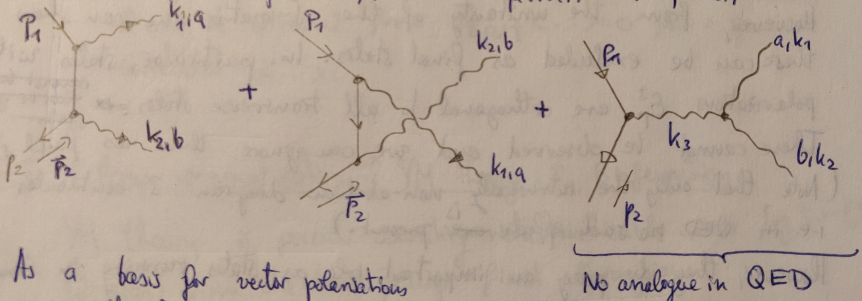
\includegraphics[width=0.7\linewidth]{gfx/YMpictures/YMfermionantifermionAnnihilation}
	\caption{Fermion and Anti-fermion annihilation processes in YM}
	\label{fig:ymfermionantifermionannihilation}
\end{figure}


As a basis for vector polarization consider the following:
\begin{equation*}
	k^2=0,\quad i.e. k^\mu = (k^0,\vec{k})\quad + \quad k^\mu\epsilon_\mu=0
\end{equation*}
satisfied for
\begin{enumerate}
	\item $\epsilon_{T,i}=(0,\vec{\epsilon}_i)^T$ with $\vec{k}\cdot\vec{\epsilon}_i$, $i=1,2,$: the transverse polarizations
	\item \begin{equation*}
		\epsilon^+ := \left(\frac{k^0}{\sqrt{2}\abs{\vec{k}}}, \frac{\vec{k}}{\sqrt{2}\abs{\vec{k}}}\right)^T\quad \text{forward light-like}.
	\end{equation*}
In addition we have 
\begin{equation*}
	\epsilon^- := \frac{1}{\sqrt{2}\abs{\vec{k}}}\left(k^0, -\vec{k}\right)^T \quad \text{backward light-like, but } k\cdot \epsilon^- \neq 0
\end{equation*}
with
\begin{align*}
	\epsilon^T_i \cdot \epsilon^T_j &= - \delta_{ij},\quad \epsilon^+\cdot \epsilon^T_i = 0 = \epsilon^- \cdot \epsilon^T_i,\\
	(\epsilon^+)^2 &=0= (\epsilon^-)^2,\quad \mI=\epsilon^+ \cdot \epsilon^-,\\
	\eta\munu &= \epsilon^-_\mu (\epsilon^+_\nu)^* + \epsilon^+_\mu (\epsilon^-_\nu)^* - \sum_{i=1,2} \epsilon^T_{i\mu} (\epsilon^T_{i\nu})^*.
\end{align*}

\end{enumerate}
Denote the amplitude by
\begin{equation}
	i M = i M^{\mu \nu} \epsilon^*_\mu(k_1) \epsilon^*_\nu(k_2)
\end{equation}
for outgoing vector polarization $\epsilon^*_\mu(k_i)$.\\
An explicit computation gives
\begin{align}
	iM^{\mu \nu} (\epsilon^T_\mu(k_1))^* (\epsilon^T_\nu(k_2 ))^* &\neq 0 \text{ both final bosons transverse}\\
	iM^{\mu \nu} (\epsilon^T_\mu(k_1))^* (\epsilon^\pm_\mu(k_2))^* &=0 \; 1 \text{ final boson null!}, \text{  but}\\
	iM^{\mu \nu} (\epsilon^+_\mu(k_1))^* (\epsilon^-_\nu(k_2))^* &\neq 0 \text{ !}
\end{align}
As in QED, the asymptotic states naively include negative norm states for time-like and zero-normstates for longitudinal polarizations. In addition, there are zero norm states in the ghost sector. However, from the unitarity of the S-matrix one can show that these can be excluded as final states. In particular, states with polarizations $\epsilon^\pm_\mu$ are orthogonal to all transverse states. These cannot be observed and we can ignore them as final states. (Note that only the intrinsically non-abelian diagram $3$ contributes to this, i.e. in QED no such effect is present.)\\
However, they do play an important role as states running loops
\begin{figure}[h!]
	\centering
	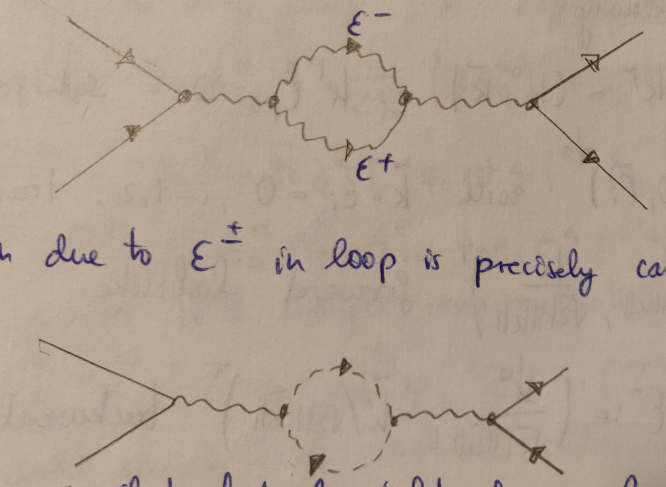
\includegraphics[width=0.7\linewidth]{gfx/YMpictures/YMghostloops}
	\caption{Ghost loops}
	\label{fig:ymghostloops}
\end{figure}


. The contribution due to $\epsilon^\pm$ in the loop is precisely cancelled by a ghost loop
if we take into account that ghost loops (like fermion loops) carry an extra factor of $(-1)$ due to their Grassmann nature.
\begin{mybox}{Ghost Fields}
	Conclusion:\\
	As advocated, ghost-fields cancel loop contributions due to unphysical vector bosons and thus serve as ’\emph{negative degrees of freedom}’.
\end{mybox}
\begin{mybox}{Slavnov-Taylor identity in YM, outlook}
	As demonstrated, in YM theory the relation
	\begin{equation}
	\label{eq:wardidQED}
		k_\mu M^\mu =0
	\end{equation}
	does in general not hold. In QED, \ref{eq:wardidQED} is a consequence of the Ward-Takahashi identity for the conserved current
	\begin{equation}
		\gamma^\mu = \bar{\psi} \gamma^\mu \psi.
	\end{equation}
	In YM, the conserved current is more complicated as it includes also $A^\mu$ itself (due to $A^3,A^4$ terms). The analogue of the Ward identities are the Slavnov-Taylor identities:\\
	Thee are the Ward Takahashi identities for $J^\mu_{BRST}$ and can be obtained from $\delta_{BRST}\expval{\dots} =0$ for a general correlator $\expval{\dots}$.
\end{mybox}
\subsubsection{Emission}

\begin{equation}
	 \feynmandiagram[horizontal=v to w]{a[particle=$\beta$] --[fermion, momentum=\(p_2\)]v --[fermion, momentum=\(p_1-k_1\)] w--[gluon, momentum=\(k_1\)] b[particle=${(a,\mu)}$], c[particle=$\alpha$]--[anti fermion, momentum=\(p_1\)] w, v--[gluon, momentum=\(k_2\)] d [particle=${(b,\nu)}$]};
\end{equation}
has the following amplitude via Feynman rules
\begin{align}
	iM&=\bar{v}^i_\alpha(p_1) i g \gamma^\mu T^a_r \epsilon^{a,\dagger}_\mu(k_1) \left(\frac{i}{\slashed{q}-m}\right)_{\alpha \beta} \delta_{ij}\epsilon^{b,*}_\nu(k_2) i g \gamma^\nu T^b_r u^j_\beta(p_2).
\end{align}
Use 
\begin{equation*}
(\slashed{p}_2-m)u(p_2)=0\quad \bar{v}(p_1) (\slashed{p}_1+m) =0, \; \mu\neq \nu \Rightarrow \; \gamma^\mu \gamma^\nu=- \gamma^\nu \gamma^\mu.
\end{equation*}
\subsubsection{Tricks in computation of scattering amplitudes}
\begin{enumerate}
	\item If computing loops with Lorentz indices, then decide which vertex (left or right) to have covariant and the other to have contravariant indices, e.g.
	\begin{equation*}
		\feynmandiagram[horizontal=v to w]{a--[gluon] v [particle=$v_1$]--[half left,gluon] w[particle=$v_2$]--[gluon]b, w--[half left, gluon] v };
	\end{equation*}
could have the following vertex structure
\begin{equation*}
	\underbrace{f^{adc} [\eta^\mu_\sigma(\dots)_\rho + \dots]}_{v_1} \underbrace{f^{bcd}[\eta^{\rho \nu} (\dots)^\sigma \dots]}_{v_2}.
\end{equation*}
\item For loop computation, only use the propagator in slimmed form as no indices/external legs present
\begin{align*}
	\feynmandiagram{a[particle=${(a,\mu)}$] --[gluon]c--[gluon] b [particle=${(b,\nu)}$]}; &= \frac{-i}{p^2+i\epsilon}\left(\eta\munu-(1-\xi) \frac{p_\mu p_\nu}{p^2}\right)\delta^{ab} \\
	\rightarrow \quad \feynmandiagram{a--[half left, gluon, edge label=$p+q$] b};&= \frac{-i}{(p+q)^2}.
\end{align*}
\item Compute the self loop
\begin{equation*}
	\feynmandiagram{a[particle=${(a,\mu)}$]--[gluon]m--[gluon, edge label=${d,\sigma}$] v--[edge label=${c,\rho}$,gluon]n--[gluon] b [particle=${(b,\nu)}$], v--[loop,min distance=2cm, gluon] v};
	\end{equation*}
as a $4$-vertex with $\sigma=\rho$ and $d=c$.
\item Trick for nasty loop integral
\begin{equation*}
	\int \frac{\md^d p}{(2 \pi)^d} \frac{1}{p^2} = \int \frac{\md^d p}{(2 \pi)^d} \underbrace{\frac{1}{p^2} \frac{1}{(p+q)^2}}_{=\frac{1}{AB}} (p+q)^2.
\end{equation*}
\item ghost loops $\Rightarrow \cdot (-1)$.
\end{enumerate}

















\subsection{$1$-Loop renormalization of YM-theory and Beta-function}
YM theory is power-counting renormalizable since $[g]=0$.\\
We start from the bare gauge-fixed Lagrangian
\begin{align*}
	\mL &= - \frac{1}{4} \left(\partial_\mu A^a_{0\;\nu} - \partial_\nu A^a_{0 \; \mu} \right)^2 - \frac{1}{2 \xi_0} (\partial A^a_0)^2 + \bar{\psi}_0 (i \slashed{\partial} - m_0) \psi_0 \\
	& - \bar{c}_c \partial_\mu \partial^\mu c_0 - g_0 A_{0\mu} \bar{\psi}_0 \gamma^\mu T^a \psi_0 + g_0 f^{abc} (\partial_\mu A^a_{0\nu}) A^{b\mu}_0 A^{c \nu}_0 \\
	&-\frac{1}{4} g^2_0 f^{abc} f^{ade} A^{\mu b}_0 A^{\nu c}_0 A^d_{\mu 0} A^e_{\nu 0} + g_0 \bar{c}_0 f^{abc} \partial^\mu A^b_{0 \mu} c^c_0
\end{align*}
and we perform field strength renormalizations
\begin{equation}
	A_0 = \sqrt{Z_3}A, \; \xi_0=Z_3 \xi, \; \psi_0= \sqrt{Z_2}\psi, \; \stackrel{(-)}{c}_0 = \sqrt{Z^c_2} \stackrel{(-)}{c}.
\end{equation}
This gives eight counterterms - not all independent:
\begin{align*}
	\delta_2 &=Z_2 -1, \; \delta_3 = Z_3-1, \; \delta^{(c)} = Z^{(c)}_2 -1, \; \delta_m = Z_2 m_0 -m,\\
	 \delta_1 &= \frac{g_0}{g} Z_2 \sqrt{Z_3}-1, \delta^{cubic}_1 = \frac{g_0}{g} Z^{3/2}_3-1,\\
	  \delta^{quartic}_1 &= \frac{g_0}{g}Z^2_3-1, \; \delta^{(c)}_1 = \frac{g_0}{g} Z^c_2 \sqrt{Z_3}-1.
\end{align*}
Note: Due to renormalization of $\xi_0$, the kinetic counterterm for $A_\mu$ becomes independent of $\xi$
\begin{equation*}
	-\frac{1}{4} \delta_3 ( \partial_\mu A_\nu - \partial_\nu A_\mu)^2.
\end{equation*}
Thus, among others, we have the counterterms
\begin{align}
	\feynmandiagram[horizontal=a to b]{a [particle=$A$] -- [gluon] c [crossed dot] --[gluon] b [particle=$b$]};
	&= -i (k^2 \eta^{\mu \nu} - k^\mu k^\nu) \delta^{ab} \delta_3 \\
	\feynmandiagram[horizontal=a to b]{a [particle=$i$] --[anti fermion] c [crossed dot] -- [anti fermion] b [particle=$j$]};
	&= i \gamma^\mu p_\mu \delta_2 \delta_{ij} \\
	\feynmandiagram[horizontal=a to b]{a -- [fermion] v [crossed dot] -- [anti fermion] b, c [particle=${(\mu,a)}$] --[boson] v};
	&= -ig T^a \gamma^\mu \delta_1
\end{align}
and in addition those for $A^3,A^4, \bar{c} A c+\bar{c} c$ $\& \psi$-mass.+
\\
\\
Our Aim is to extract the $1$-loop $\beta$-function for $g$.\\
Since $\beta(g)$ is sensitive only to UV-divergences, we can henceforth set $m=0$. As in QED, we extract $\beta(g)$ from the Callen-Symancyk equation for the $3$-point function $\expval{A\bar{\psi} \psi}$ as
\begin{equation}
\beta(g) = g \mu \frac{\partial}{\partial \mu} \left(-\delta_1 + \delta_2 + \half \delta_3\right) \quad \text{at $1$-loop}.
\end{equation}
We therefore only need the $mu$-dependence of $\delta_1,\delta_2,\delta_3$. We will see that after cancellations all divergences are of the form 
$\frac{\Gamma(2-\frac{\md}{2})}{\Delta^{2-\frac{\md}{2}} }$ in dimensional regularization with $\Delta$ some $p^2$-invariant. We can identify
\begin{equation}
	\mu^2 = \Delta
\end{equation}
by choice of renormalization conditions and extract only the divergences of $\delta_i$ for $\beta(g)$.



 \subsubsection{Preliminaries in Group Theory}
Given a representation $R$ with $T^a_R \equiv (T^a_R)_{ij}$, $i,j=1,\dots,\dim R$, i.e. a matrix representation, of a Lie algebra $Lie(H)$ with dimension $\dim H$, the \emph{second Casimir} $C_2(R)$ is defined via 
\begin{equation}
	\sum_a T^a_R T^a_R = T^a_R T^a_R= C_2(R) \cdot \mI.
\end{equation}
If we normalize the $T^a_R$ such that
\begin{equation}
	\tr T^a_R T^b_R = \underbrace{C(R)}_{\text{normalization group factor}} \delta^{ab}
\end{equation}
then
\begin{equation}
	\dim(R) C_2 (R) = C(R) \cdot \dim(H).
\end{equation}
Consider the examples
\begin{enumerate}
	\item Let $R=f$ be the fundamental representation of $SU(N)$ normalized such that\begin{equation}
		\tr(T^a_f T^b_f) = \half \delta^{ab} \quad \Rightarrow \quad C(f) = \half.
	\end{equation}
	Then 
	\begin{equation}
		C_2(f) = \half \frac{\dim(SU(N)) }{\dim(f)} = \half \frac{N^2-1}{N}.
	\end{equation}
	\item Let $R=Ad$ be the adjoint representation of $H$, defined such that 
	\begin{equation}
		(T^b_{Ad})_{ac} = i f^{abc} \quad \Rightarrow \quad C(H) := C(Ad)
	\end{equation}
	computable via
	\begin{align*}
		C(H)\delta^{ab} &= \tr(T^a_{Ad} T^b_{Ad})= -f^{dac} f^{cbd},\quad C(H) \delta^{ab} = f^{acd} f^{bcd} \\
		 C_2(H) \delta^{ab} &= (T^a_{Ad})_{bc} (T^a_{Ad})_{cd} = f^{cab} f^{cae} \\
		\Rightarrow \quad C(H) & = C_2(H),
	\end{align*}
also follows since $\dim(Ad)=\dim(H)$. For example, $H=SU(N)$ gives us 
\begin{equation*}
	C(SU(N)) = N.
\end{equation*}
\end{enumerate}



\subsubsection{Computation of $\delta_3$}
\begin{figure}[h!]
	\centering
	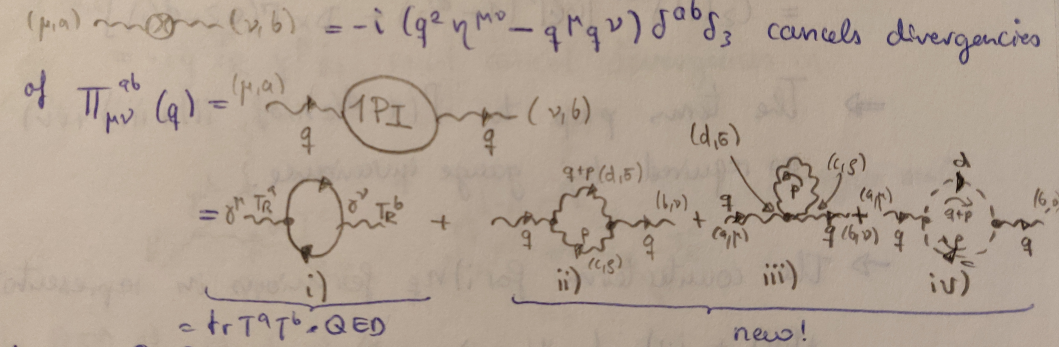
\includegraphics[width=0.5\linewidth]{gfx/YMpictures/YMselfenergy}
	\caption{YM self-energy renormalization}
	\label{fig:ymselfenergy}
\end{figure}
As in QED, \begin{equation}
	q^\mu \Pi\munu(q)=0,
\end{equation}
which is a consequence of the Slavnov-Taylor identities. So we have
\begin{equation*}
	\Pi\munu(q)=i (q^2 \eta^{\mu \nu} - q^\mu q^\nu) \Pi(q^2).
\end{equation*}
Thus, compute the four diagrams $i)-iv)$ to find $\delta_3$:
\begin{enumerate}
	\item[i)] Choosing $\Delta:= -x(1-x)q^2$ with renormalization scale $\mu$, we find
	\begin{equation}
		\delta_3 |_{i)} = -\frac{g^2}{(4 \pi)^2} \frac{4}{3} C(R) \frac{\Gamma(2-\frac{\md}{2})}{(\mu^2)^{2-\frac{\md}{2}}}
	\end{equation}
	for a fermion in representation $R$.\\
	\\
	Note that the pure YM diagrams $ii)-iv)$ (pure in the sense that they do not appear in QED) are computed in Feynman gauge $\xi=1$.
	\item[ii)] Contains two types of divergences, via dimensional Regularization:
	\begin{enumerate}
		\item $\Gamma(2-\frac{\md}{2})\times \dots \leftrightarrow$ corresponds to logarithmic divergences in $\md=4$.
		\item $\Gamma(1-\frac{\md}{2})\times \dots \leftrightarrow$ corresponds to logarithmic divergence in $\md=2$, i.e. $\int \frac{\md^{\md} p}{(p^2)}$ and thus a quadratic divergence in $\md=4$.
	\end{enumerate}
A quadratic divergence would indicate a renormalization of the gauge boson mass, which is forbidden by gauge invariance. This term must hence cancel against other contributions.
\item[iii)]
\begin{equation}
	iii)= \left[A \cdot \Gamma(1-\frac{\md}{2}) + B\cdot \Gamma(2-\frac{\md}{2}) \right] C_2(H) \delta^{ab} 
\end{equation}
\item[iv)]
We get a $(-1)$ sign from Grassman fields in loop
\begin{align}
	iv)&= (-1) \int \frac{\md^4p}{(2 \pi)^4} \frac{i}{p^2} \frac{i}{(p+q)^2} g^2 f^{dac} (p+q)^\mu f^{cbd} p^\nu \nonumber \\
	&= C_2(H) \delta^{ab} \left[C \cdot \Gamma(1-\frac{\md}{2}) + D\cdot \Gamma(2-\frac{\md}{2})\right].
\end{align}
\end{enumerate}
The terms proportional to $\Gamma(1-\frac{\md}{2})$ of $ii)+iii)+iv)$ precisely cancel - as required by gauge invariance.
\\
Thus, the counterterm for $1)$ $n_f$ fermions in Representation $R_f+2)+3)+4)$ (with $\Delta= \mu^2$) is
\begin{equation}
	\delta_3 = \frac{g^2}{(4 \pi)^2} \frac{\Gamma(2-\frac{\md}{2})}{(\mu^2)^{2-\frac{\md}{2}}} \left[\frac{5}{3} C_2(H) - \frac{4}{3} n_f C(R_f)\right].
\end{equation}



 \subsubsection{Computation of $\delta_2$}
 
\begin{figure}[h!]
	\centering
	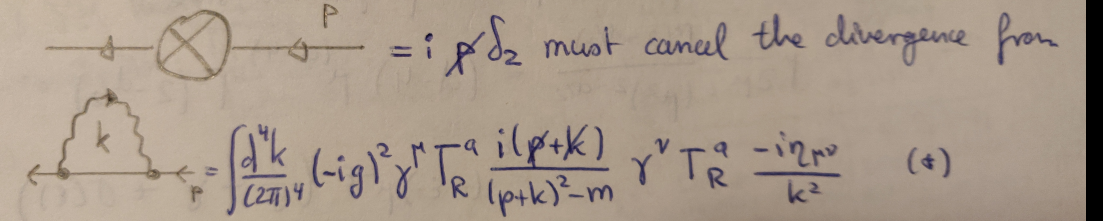
\includegraphics[width=0.7\linewidth]{gfx/YMpictures/YMoneLoopDelta2}
	\caption{}
	\label{fig:ymoneloopdelta2}
\end{figure}
 Since we only need the UV divergences, we set again $m=0$.
 \\The group theory factor is $T^a_R T^a_R = C_2(R) \cdot \mI$, thus
 \begin{align}
 	\ref{fig:ymoneloopdelta2} &= C_2(R)\mI  \times \left(\feynmandiagram[horizontal=a to b]{a--c--d--b, c--[boson, half left]d};\right)|_{QED} \\
 	&= C_2(R) \frac{i g^2}{(4 \pi)^{\frac{\md}{2}} } \slashed{p} \int_0^1 \md x (1-x)(\md -2 ) \frac{\Gamma(2-\frac{\md}{2})}{\Delta^{2-\frac{\md}{2}}}
 \end{align}
with $\Delta=-x(1-x)p^2$.\\ 
Identifying $\Delta=\mu^2$ yields
\begin{equation}
	\delta_2 = - \frac{g^2}{(4 \pi)^2} \frac{\Gamma(2-\frac{\md}{2})}{(\mu^2)^{2-\frac{\md}{2}} } C_2(R).
\end{equation}


\subsubsection{Computation of $\delta_1$}
\begin{figure}[h!]
	\centering
	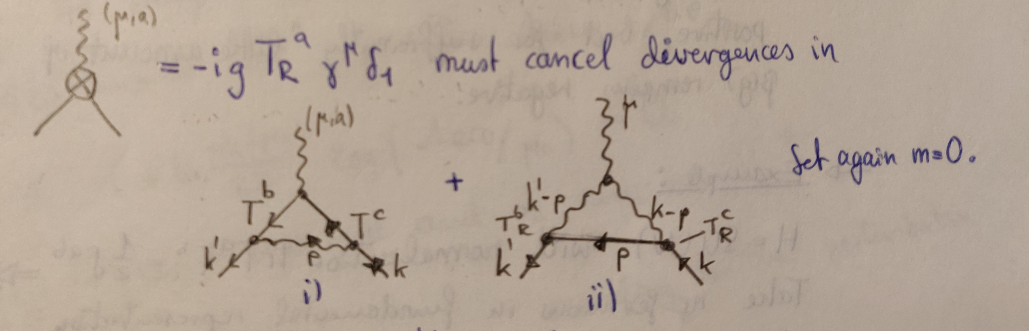
\includegraphics[width=0.7\linewidth]{gfx/YMpictures/YMoneLoopDeltaOne}
	\caption{}
	\label{fig:ymoneloopdeltaone}
\end{figure}
Consider the two separate diagrams individually
\begin{enumerate}
	\item[i)] In QED the Ward identities imply $\delta_1 |_{QED} = \delta_2|_{QED}$. We can factorize the diagram into contributions from YM and QED similar interactions like the following with this identity
	\begin{equation}
		\delta_1 |_{i)} = \underbrace{- \frac{g^2}{(4 \pi)^2} \frac{\Gamma(2-\frac{\md}{2})}{(\mu^2)^{2-\frac{\md}{2}} }}_{= T^a_R \cdot ({i)}_{QED})} \left(C_2(R)-\half C_2(H)\right),
	\end{equation}
	where we used the results from our QED calculations and just included the group theory factor..
	\item[ii)] Applying the same logic here, we find
	\begin{equation}
		\delta_1 |_{ii)} = -\frac{g^2}{(4 \pi)^2} \frac{\Gamma(2-\frac{\md}{2})}{(\mu^2)^{2-\frac{\md}{2}} } \frac{3}{2} C_2(H).
	\end{equation}
\end{enumerate}
Altogether
 \begin{equation}
 	\delta_1 = - \frac{g^2}{(4 \pi)^2} \frac{\Gamma(2-\frac{\md}{2})}{(\mu^2)^{2-\frac{\md}{2}}} \left[C_2(R)+C_2(H)\right].
 \end{equation}
 
 \subsubsection{YM  $\beta$-function at $1$-loop in $g$}
The final result is found by noting that the divergencies vanish for the computation of the $\beta$-function since
\begin{align*}
	\mu \frac{\partial}{\partial \mu} \frac{\Gamma(2 -\frac{\md}{2})}{(\mu^2)^{2-\frac{\md}{2}} } &= (\md -4) \mu^{(\md-4)} \Gamma(2-\frac{\md}{2}) \\
	&\stackrel{\md=4-\epsilon}{=} (-\epsilon) \mu^{-\epsilon} \left(\frac{2}{\epsilon} -\gamma + \mO(\epsilon)\right) \\
	&\stackrel{\epsilon\rightarrow 0}{=} -2.
\end{align*}
\begin{mybox}{YM $\beta$ function to leading order in $\md=4$}
	\begin{equation}
		\label{eq:betafunctionYangMills}
		\beta^{(1)}_{YM}(g) = - \frac{g^3}{(4 \pi)^2} \left[\frac{11}{3} C_2(H) - \frac{4}{3} n_f C(R_f)\right].
	\end{equation}
\end{mybox}
\subsubsection{Crucial Implications}
\begin{enumerate}
	\item \begin{mybox}{Asymptotic freedom}
	Pure non-abelian YM theory is \emph{asymptotically free} since $\beta(g)<0$ and thus $g\rightarrow 0$ as $\mu \rightarrow\infty$.
	\end{mybox}
\item \begin{mybox}{}	
	Of all known renormalizable QFTS in $D=4$, YM theory is the only one which is asymptotically free!
	Strictly speaking, it is the only one for which the UV cut-off $\Lambda$ can be taken to $\infty$ in perturbation theory.
\end{mybox}
	\item Coupling YM to fermionic matter tends to make $\beta(g)$ positive, but for sufficiently "little amount of fermions" $\beta(g)$ remains negative.
\end{enumerate}
\subsubsection{Examples}
$H=SU(N)$ with normalization 
\begin{equation}
	\tr(T^a T^b) = \half \delta^{ab} \quad \Rightarrow \quad  C_2(SU(N)) = N.
\end{equation}
Now take $n_f$ fermions in fundamental representation
\begin{equation*}
	R_f = \yng(1) \quad \text{with} \quad C\left(\yng(1)\right)=\half.
\end{equation*}
Then, the $\beta$-function of this theory at $1$-loop reads
\begin{equation}
	\beta(g) = -\frac{g^3}{(4\pi)^2} \left[\frac{11}{3} N-\frac{2}{3}n_f\right].
\end{equation}
We will use this below to find the beta function of QCD.
\subsubsection{Notes on the $\beta$ function}
Generally, to one-loop/leading order in $\lambda$, the beta function becomes
\begin{equation*}
	\beta(\lambda) = \mu \frac{\partial}{\partial \mu} \left(-\delta_{\lambda}+\frac{\lambda}{2} \sum_i \delta_{Z_i}\right)
\end{equation*}
and in non-abelian gauge theory with a renormalization scale $M$
\begin{equation*}
	\beta(g) = g M\frac{\partial}{\partial M} \left(-\delta_1+\delta_2+\frac{\delta_3}{2} \right)
\end{equation*}
which is also the $\beta(g)$ for $3$-point function $\expval{A\bar{\psi}\psi}$ at $1$-loop.
\subsection{Quantumchromodynamics (QCD)}
\subsubsection{The theory}
QCD is a $SU(3)$ YM theory
\begin{equation}
	\label{eq:qcdlagrangian}
	\mL_{QCD} = \bar{\psi}_i \left[i(i\gamma^\mu D_\mu)_{ij}-m \delta_{ij}\right]\psi_j - \frac{1}{4} F^a\munu F^{\mu \nu, a}
\end{equation}
where $\psi_i(x)$ is the quark field in the fundamental representation of the $SU(3)$ gauge group, indexed by $i,j,\dots$. The YM $SU(3)$ theory is therefore coupled to $6$ quarks in fundamental representation
\begin{equation}
q^{(f)} \equiv q^{(f)}_i,
\end{equation}
where $i=1,2,3$ are the \emph{colour indices} of the fundamental of $SU(3)$ (red,yellow,blue) and $f=1,\dots,6$ are the \emph{flavour indices} called $u,d,c$,$s,t,b$\\ The Dirac matrices $\gamma^\mu$ connect the spinor representation to the vector representation of the Lorentz group. The symbol $F^a\munu$ represents the gauge invariant gluon field strength tensor. It is given by $F^a\munu = \partial_\mu A^a_\nu$$ - \partial_\nu A^a_\mu +g f^{abc} A^b_\mu A^c_\nu$, where $A^a_\mu(x)$ are the gluon fields in the adjoint representation of the $SU(3)$ gauge group, indexed by $a,b,\dots$. The variables $m$ and $g$ correspond to the quark mass and coupling of the theory, which are subject to renormalization.\\
 Quarks are massive spin $\half$ fermions which carry a colour charge whose gauging is the context of QCD. Quarks are represented by Dirac fields in the fundamental representation of $SU(3)$. They also carry electric charge (either $-1/3$ or $2/3$) and participate in weak interactions as part of the weak Isospin doublets.\\
Gluons are spin $1$ bosons which also carry colour charges, since they lie in the adjoint representation of $SU(3)$. They have no electric charge, do not participate in the weak interactions and have no flavour.\\
QCD gives rise to three basic interactions
\begin{enumerate}
	\item A quark may emit (or absorb) a gluon,
	\item A gluon may emit (or absorb) a gluon,
	\item and two gluons may directly interact.
\end{enumerate}
This contrasts with QED, in which only the first kind of interaction occurs, since photons have no charge. Diagrams involving FP-ghosts must be considered too.
.\\
\\
QCD is not a conformal field theory, since $\mL_{QCD}$ contains dimensionful coupling, in particular the fermionic mass $m_\psi$. This introduces a scale into the theory that makes i non-conformal. QCD($m_f=0$) is still not conformal, since massless QCD has an extra symmetry, namely \emph{Chiral symmetry}, but the coupling of the gauge potential to the fermions still needs to be renormalized, i.e. is scale-dependent.\\
The fermion-gauge field interaction temr is given by $g \bar{\psi} \gamma^\mu A_\mu \psi$ where the coupling $g$ has mass dimension zero in $D=4$ dimensions.\\
Note
\begin{equation*}
	[S]=0\Rightarrow\;[\mL_{QCD} ] = 4, [\psi]=\frac{3}{2} \& [A]=1, \; 2[\psi] + [A] = 4 \; \Rightarrow \; [g] =0
\end{equation*}
Repeating the above in other words, QCD is not conformal since it has a negative $\beta$-function 
\begin{equation}
	\beta(g) = -\frac{g^3}{(4 \pi)^2} \left[11-\frac{2}{3} n_f\right]
\end{equation}
where $n_f=6$ is the number of quark flavours. Thus,
\begin{equation}
	\beta_{QCD}(g) = -\frac{7}{16 \pi^2} g^3 \quad <0.
\end{equation}
\subsubsection{Running coupling and $\beta$-function}
Using our result for the $1$-loop YM beta function \ref{eq:betafunctionYangMills} we have
\begin{equation}
	\beta(g) = -\frac{g^3}{(4 \pi)^2} b_0+ \mO(g^5)
\end{equation}
with
\begin{equation}
	b_0=\left(\frac{11}{3}\cdot 3 - \frac{2}{3} \cdot 6\right) = 7
\end{equation}
which comes from $N=3$ for $SU(3)$ and $n_f=6$ quarks being contained in our theory.\\
\begin{mybox}{QCD Running Coupling}
	Note that $\alpha_s =\frac{g^2}{4 \pi}$ runs as
	\begin{equation}
		\label{eq:qcdrunningcoupling}
		\alpha_s(\mu) = \frac{\alpha_s(\mu_0)}{1 + b_0 \frac{\alpha_s(\mu_0)}{2 \pi} \ln(\frac{\mu}{\mu_0})}.
	\end{equation}
	Experimentally for $\mu_0\approx 91.2$ GeV (the mass of the $Z^0$-boson) we have $\alpha_s(\mu_0)\approx 0.118$.\\
\end{mybox}
\begin{mybox}{Conformal anomaly of QCD}
		Even thought QCD is conformally invariant, the non-vanishing $\beta$-function in the quantum theory means that the colour coupling needs to be renormalized and so the theory suffers from a  \emph{conformal anomaly}.
\end{mybox}
Define the strong scale $\Lambda_{QCD}$ such that at $1$ loop
\begin{equation}
	\alpha_s(\mu) \rightarrow \infty \quad \text{as} \quad \mu \stackrel{>}{\rightarrow} \Lambda_{QCD},
\end{equation}
i.e. via
\begin{equation*}
	1+b_0 \frac{\alpha_s(\mu_0)}{2 \pi} \ln(\frac{\Lambda_{QCD}}{\mu_0}) =0.
\end{equation*}
Then $\Lambda_{QCD} \approx 200$MeV and $\alpha_s$ runs as 
\begin{figure}[h!]
	\centering
	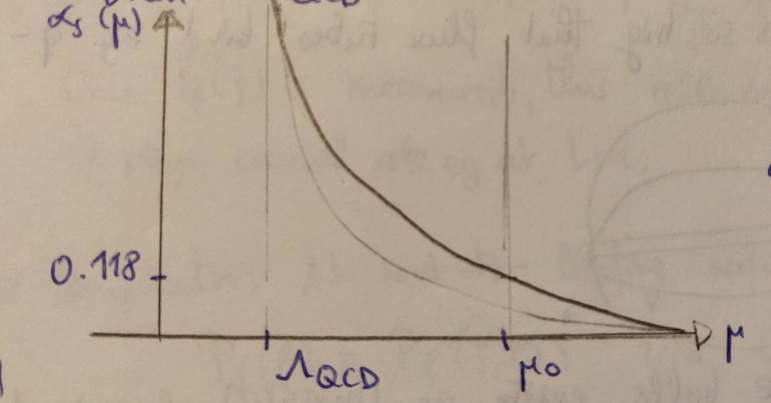
\includegraphics[width=0.7\linewidth]{gfx/YMpictures/QCDrunningcoupling}
	\caption{Running coupling of QCD}
	\label{fig:qcdrunningcoupling}
\end{figure}








according to the perturbative analysis.
\\
Perturbation theory is valid only for processes at typical energies at $\geq 1$GeV; below that use non-perturbative methods (e.g. lattice QCD, a numerical approach to solve the path-integral due to Wilson) must be used, and they confirm that $\alpha_s$ becomes strong in the IR.
\subsubsection{Phase structure}
QCD exhibits an intricate phase structure, including $2$ phases:
\begin{enumerate}
\item Deconfined phase (asymptotically free):\\
For energies $\gg \Lambda_{QCD}$, QCD is weakly coupled. The observables particles are the free quarks and gluons $g^{(a)}$, $a=1,\dots,8$ ($\equiv$ QCD gauge bosons).
\item Confined phase (=\emph{hadronic phase}):\\
The observable degrees of freedom are bound states of quarks, anti-quarks and gluons, they are all given by colour singlets.\\
From
\begin{enumerate}
	\item Quarks $q_i$ in fundamental, i.e.
	\begin{equation}
		q_i \rightarrow U^{\;j}_i q_j,\quad U\in SU(3),
	\end{equation}
	and
	\item Anti-quarks $\bar{q}^i$ in anti-fundamental, i.e.
	\begin{equation}
		\bar{q}^i \rightarrow \bar{q}^j (U^\dagger)^i_{\;j},
	\end{equation}
\end{enumerate}
we can form two types of $SU(3)$ singlets
\begin{enumerate}
	\item Mesons:
	\begin{equation}
		q_i \bar{ q}^i \rightarrow q_i U^{\;j}_i (U^\dagger)^i_{\;k} \bar{q}^k = q_i \bar{q}^i,
	\end{equation}
	and
	\item Baryons:
	\begin{equation}
		\epsilon^{ijk} q_i q_j q_k \rightarrow \underbrace{(\det(U))}_{=1} \epsilon^{ijk} q_i q_j q_k.
	\end{equation}
\end{enumerate}
\end{enumerate}
The physical picture is the following:\\
QCD exhibits an intricate phase structure, including $2$ phases:
\begin{enumerate}
	\item Deconfined phase (asymptotically free):\\
	For energies $\gg \Lambda_{QCD}$, QCD is weakly coupled. The observables particles are the free quarks and gluons $g^{(a)}$, $a=1,\dots,8$ ($\equiv$ QCD gauge bosons).
	\item Confined phase (=\emph{hadronic phase}):\\
	The observable degrees of freedom are bound states of quarks, anti-quarks and gluons, they are all given by colour singlets.\\
	From
	\begin{enumerate}
		\item Quarks $q_i$ in fundamental, i.e.
		\begin{equation}
		q_i \rightarrow U^{\;j}_i q_j,\quad U\in SU(3),
		\end{equation}
		and
		\item Anti-quarks $\bar{q}^i$ in anti-fundamental, i.e.
		\begin{equation}
		\bar{q}^i \rightarrow \bar{q}^j (U^\dagger)^i_{\;j},
		\end{equation}
	\end{enumerate}
	we can form two types of $SU(3)$ singlets
	\begin{enumerate}
		\item Mesons:
		\begin{equation}
		q_i \bar{ q}^i \rightarrow q_i U^{\;j}_i (U^\dagger)^i_{\;k} \bar{q}^k = q_i \bar{q}^i,
		\end{equation}
		and
		\item Baryons:
		\begin{equation}
		\epsilon^{ijk} q_i q_j q_k \rightarrow \underbrace{(\det(U))}_{=1} \epsilon^{ijk} q_i q_j q_k.
		\end{equation}
	\end{enumerate}
\end{enumerate}
The physical picture is the following:\\
The strong force is so big that flux tubes bind e.g. $q-\bar{q}$ pairs together.



\begin{figure}[h!]
	\centering
	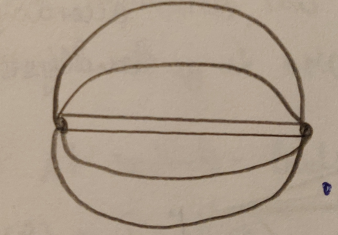
\includegraphics[width=0.7\linewidth]{gfx/YMpictures/GlueTunnel}
	\caption{}
	\label{fig:gluetunnel}
\end{figure}

In addition, glue balls exist as (mainly) gluonic bound states. To date, no analytic derivation of the hadronic spectrum starting from QCD is known.
\newpage
\subsubsection{Deep-inelastic scattering - Parton theory}
A useful concept for hard, i.e. high-energy scattering involving hadrons is given by the parton distribution functions:
\begin{mybox}{Parton distribution function PDF}
	Consider some hadron with momentum $P$. Then the parton-distribution function $P_F(\xi)$ is \\
	$P_f(\xi)\md \xi:=$ \emph{probability ot find a constituent $f$ ((anti-)quark or gluon) inside hadron with momentum} $p=\xi \cdot P$.
\end{mybox}
To leading order in $\alpha_s$, $P_f(\xi)$ is independent of energy scale $Q$ at which the hadron is analysed and can be determined by deep-inelastic scattering experiments of the form 

\begin{figure}[h!]
	\centering
	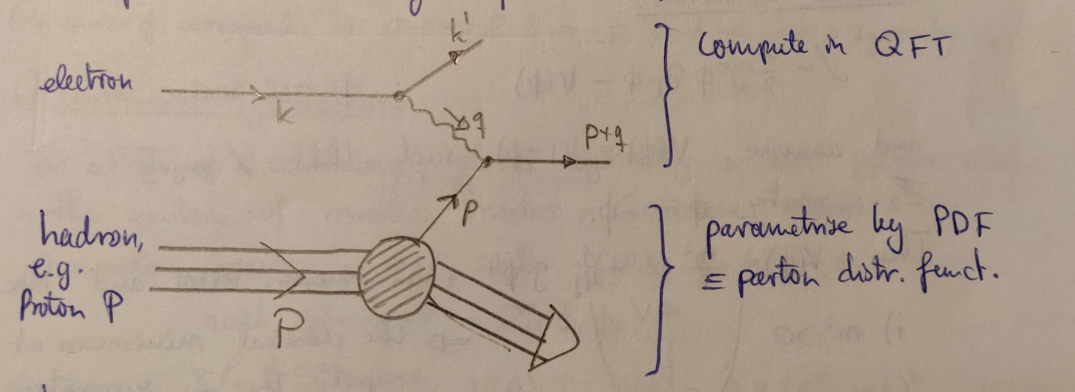
\includegraphics[width=0.7\linewidth]{gfx/YMpictures/PartonScattering}
	\caption{Parton scattering process}
	\label{fig:partonscattering}
\end{figure}










via
\begin{equation}
	\sigma(e^-(k)p(P) \rightarrow e^-(k^\prime)+X) = \int_0^1 \md \xi \sum_f P_f(\xi) \sigma\left(e^-(k) q_f( \xi p) \rightarrow e^-(k^\prime) +q_f(p^\prime)\right).
\end{equation}
Once $P_f(\xi)$ is measured, this allows for predictions for other experiments and plays a crucial role at e.g. the LHC.\\
\\
Complication:\\
At next-to-leading order, $P_f(\xi)$ is a function $P_f(\xi)\equiv P_f(\xi,Q)$ via $Q^2=-q^2$ (in above picture). I.e. at high momentum transfer, the baryon is probed at different energy scales and virtual $q-\bar{q}$ etc pairs become important ("\emph{Parton evolution}").






\subsection{Comments to think about}
\begin{enumerate}
	\item Non-abelian coupling constants are always asymptotically free. QED is abelian and has Landau pole on other side.
\end{enumerate}

\section{Standard Model of particle physics}
The Standard Model (SM) of particle physics is formulated as a Yang-Mills theory specified by the following data.
The gauge group of the Standard Model is 
\begin{equation}
	SU(3)_C \times SU(2)_L \times U(1)_Y.
\end{equation}
\footnote{C=\text{colour},Y=\text{Hypercharge}}
 $SU(3)_C$ describes the strong interaction, represented by QCD, with an unbroken, i.e. exact, gauge symmetry. The electroweak sector (\emph{Glashow-Weinberg-Salam} model) $SU(2)_L\times U(1)_Y$ describes electroweak interactions, i.e. two sectors which are mixed. The gauge sector of this theory is spontaneously broken to $U(1)_{QED}$ by the Higgs mechanism.\\
 \\
  The SM is a chiral theory, i.e.
 left- and righthanded fermion fields $ψ_L ≡ P_L ψ$ and $ψ_R ≡ P_R ψ$ transform in different representations. 
\\
The coupling of matter to gauge fields takes place via the covariant derivative of the SM
\begin{equation}
	D_\mu = \partial_\mu - i g_s A^a_\mu T^a_{SU(3)_C} - i g_W W^a_\mu T^a_{SU(2)_L} -i g^\prime y B_\mu,
\end{equation}
where $g_s$ is the strong coupling, $g^\prime$ the $U(1)_Y$ coupling constant, $g_W$ the $SU(2)_L$ coupling and $y$ is the hypercharge\footnote{like we have $e=Q \abs{e}$, here we do $g^\prime = g^\prime y$}. The generators are
\begin{enumerate}
	\item The one and only generator of $U(1)_Y$ is $y\mI$. Different matter fields have different values of $y$. In general due to being abelian we only know $T^{a=1}=\beta \cdot \mI$ since $[T,T]=0$, but we can choose $ T=\mI$.
	\item The generator of $SU(3)_C$ is 
	\begin{equation}
		T^a_{SU(3)_C} = \left\{ \begin{array}{ll}
		\frac{\lambda^a}{2} & \text{fundamental rep, i.e. quarks}\\
		0 & \text{singlet, i.e leptons}
		\end{array}		
		\right\}
	\end{equation}
	\item The generator of $SU(2)_L$ is 
	\begin{equation}
		T^a_{SU(2)_L} = \left\{ \begin{array}{ll}
		\frac{\sigma^a}{2}& \text{ fundamental rep., i.e. LH lepton}\\
		0 & \text{ singlet, i.e. RH lepton}
		\end{array}
		\right\}
	\end{equation}
\end{enumerate}

 
 
 
 
 
 
 
 
 
 
 
 
 
 
 The Standard Model comprises $3$ families of the following contents:
 \begin{tabular}{|l|lll|}
 	matter field          & rep. under $SU(3)_C$ & rep. under $SU(2)_L$ & rep. under $U(1)_Y=y$\\
 	\toprule
      $3\times \; Q_L$ & $\mathbf{3}$ fund. triplet eg (b,g,r)& $\mathbf{2}$ doublet & $\frac{1}{6}$\\
      $ \bar{u}_R,\bar{c}_R,\bar{t}_R$ & $\bar{\mathbf{3}}$ antifund, triplet & $\mathbf{1}$ singlet & $-\frac{2}{3}$\\
      $ \bar{d}_R, \bar{s}_R, \bar{b}_R$ & $\bar{\mathbf{3}}$ & $\mathbf{1}$& $\frac{1}{3}$ \\
  \midrule
  $e_R,\mu_R,\tau_R$ & $\mathbf{1}$ &$\mathbf{2}$ &$-\frac{1}{2}$ \\
  $\bar{ \nu}_{e,R},\bar{\nu}_{\tau,R},\bar{\nu}_{\mu,R}$ & $\mathbf{1}$ & $\mathbf{1}$ & $0$ \\
  $ \bar{e}_R,\bar{\mu}_R,\bar{\tau}_R$& $\mathbf{1}$& $\mathbf{1}$&$1$\\
  \midrule
  $H$ & $\mathbf{1}$ & $\mathbf{2}$ & $\half$\\
  \bottomrule
  $A^{QCD}_\mu$ & adjoint rep. & $\mathbf{1}$ & 0\\
  $W^{SU(2)_L}_\mu$ & $\mathbf{1}$ &adjoint rep. & 0 \\
  $B^{U(1)_Y}_\mu$ & $\mathbf{1}$& $\mathbf{1 }$& adjoint rep. \\
 \end{tabular}
where \footnote{A $0$ indicates the representation which sets everything to zero.}
\begin{enumerate}
	\item $3$ families of LH quark doublets (i.e. doublets under $SU(2)_L$)
	\begin{equation}
		Q^{i=1,2,3}_L = \begin{pmatrix}
		u^i_L\\
		d^i_L \\
		\end{pmatrix},\quad 
		\begin{pmatrix}
		c^i_L\\
		s^i_L \\
		\end{pmatrix}, \quad 
		\begin{pmatrix}
		t^i_L \\
		b^i_L \\
		\end{pmatrix},
	\end{equation}
	all of which carry a colour charge $i$ which indicates them transforming in the fundamental under $SU(3)$. 
	\item $3$ families of LH Leptons packaged as doublets under $SU(2)L$ 
	\begin{equation}
		L_L = \begin{pmatrix}
		\nu_{e_L} \\
		e_L\\
		\end{pmatrix},\quad 
		\begin{pmatrix}
		\nu_{\mu_L} \\
		\mu_L \\
		\end{pmatrix},
		\quad 
		\begin{pmatrix}
		\nu_{\tau_L} \\
		\tau_L\\
		\end{pmatrix},
	\end{equation}
	which are singlets under $SU(3)_C$, i.e. they don't carry a colour charge. We also have RH Leptons which are charged neither under $SU(3)_C$ nor $SU(2)$. Note that the RH Neutrino for all three families is absent in a minimal SM.
	\item The complex scalar Higgs field is given by a single doublet of $SU(2)_L$ 
	\begin{equation}
	H = \begin{pmatrix}
	H^+ \\
	H^0 \\
	\end{pmatrix}
	\end{equation}
	which has $4$ real degrees of freedom. We will see later that
	\begin{equation}
		\expval{H}\neq 0 \quad \Rightarrow \quad  \underbrace{SU(2)_L \times U(1)_Y}_{4 \text{ generators}}  \stackrel{SSB}{\rightarrow} \underbrace{U(1)_{QED}}_{1 \text{ generator}}
	\end{equation}
	the spontaneous breaking of $3$ generators of the electro-weak sector via the non-vanishing VEV of the SM Higgs leads to $3$ unrealized Goldstone bosons and $1$ physical Higgs. The three Goldstone bosons give rise to the longitudinal polarization of $Z^0, W^\pm$, which are massive. This is in more detail described in \ref{subsubsec:higgsSMSSB}
	\item Note that the electric charge of a particle is obtained via the sum rule
	\begin{equation}
		\label{eq:electricchargeSM}
		Q_{e} = T^3_{SU(2)_L} + y \mI_2, \quad  T^3_{SU(2)}= \left\{\begin{array}{ll}
		\begin{pmatrix}
		\underbrace{\half}_{eg. \; \nu_e} & 0 \\
		0 & \underbrace{- \half}_{eg.\; e^-} \\
		\end{pmatrix}
		& \text{if doublet }\mathbf{2}\\
		0 & \text{if singlet }\mathbf{1}\\
		\end{array}	\right\} 
	\end{equation}
\end{enumerate}

 
 
 \section{Contents of the SM}
 \subsection{Gauge fields}
 \begin{statements}
 	The number of gauge fields$=$ number of generators in Lie algebra of the corresponding gauge group.
 \end{statements}
We know that eg. $SU(N)$ has $N^2-1$ generators\footnote{Count the real degrees of freedom in a $SU(N)$ matrix, i.e. one has complex entries and thus $2 N^2$ real components, but unitarity implies $2 N^2\rightarrow N^2$ and $detU=-1$ is another condition such that $N^2-1$. }, whereas $U(1)$ has $1$ generator. 
\begin{enumerate}
	\item $SU(3)_C$ therefore has $8$ generators, which are \emph{gluons} $A^{a=1,\dots,8}_\mu$. $SU(3)_C$ is unbroken such that the gluons are massless, i.e. $m_{A^a_\mu}=0$ with $2$ spin polarizations $T_1,T_2$ or $+,-$ (where longitudinal polarization decouples due to vanishing mass.)
	\begin{statements}
		In general, any unbroken gauge theory always leads to massless gauge fields.
	\end{statements}
\item $SU(2)_L \times U(1)_Y$ has $4$ generators, i.e. $4$ gauge fields being $A^{a=1,2,3}_\mu$ for $SU(2)_L$ and $B_\mu$ for $U(1)_Y$. The SM Higgs field however breaks this gauge sector spontaneously 
\begin{equation*}
	SU(2)_L\times U(1)_Y \longrightarrow U(1)_{QED}
\end{equation*}
such that only $1$ generator is unbroken/left, i.e. the QED photon $A_\mu$. This generator is now massless but the other $3$ $W^+_\mu,W^-_\mu,Z^0$ are massive, by the Higgs mechanism, vector bosons carrying the weak interaction.
\end{enumerate}
\subsubsection{Simple Lie groups}
Consider theories invariant under $SU(N)$, which is a simple Lie group i.e. $SU(N) \neq G_1 \times G_2$. Note that $U(N)$ is a group but it is not a simple Lie group as it is isomorphic to $U(1)\times SU(N)$, which are both simple groups. \emph{Each simple group will have its own different gauge coupling} When we work with gauge theories, there is a unique coupling constant for each simple group:
\begin{align*}
	SU(2)_L& \rightarrow g_W \text{ weak coupling constant} \\
	U(1)_Y &\rightarrow g^\prime \text{ hypercharge}\\
	SU(3)_C & \rightarrow g_S \text{ strong or QED coupling}.
\end{align*}
We do not work with non-simple groups. Break groups into smallest possible decomposition of simple groups, such that we can associate a (gauge) coupling constant to each simple group.\\
To have a gauge theory, the group has to be a Lie group (i.e. a group which continuously depends on some parameters).
\begin{equation*}
	G \text{ Lie group } \Rightarrow g=\exp\left[i \sum_{a=1}^{N_G} T^a \theta^a\right] \quad \forall g\in G
\end{equation*}
where $\theta^a$ are continuous parameters and $T^a$ are the generators defining Lie group/algebra, $N_G=\#$ generators, $\{T^a\}$ satisfy the Lie algebra.
\begin{enumerate}
	\item $U(1)$ is the simplest Lie group, . Thus
	\begin{equation*}
U=e^{i\alpha}, \;\alpha \in \mR\; \forall U \in U(1 \quad \Rightarrow \;T^{a=1}=1, \theta^{a=1} = \alpha.
	\end{equation*}
\item \begin{equation*}
	U=\exp\left[i\sum_{a=1}^{N^2-1} T^a \theta^a\right]  \quad \theta^a \in \mR \forall a, U \in SU(N).
\end{equation*}
\end{enumerate}
\subsubsection{Repackaging of the gauge fields}
In fundamental representation of $SU(2)$, the generators are $T^a=\half \sigma^a$ $3$ hermitian matrices with $f^{abc} = \epsilon^{abc}$ and normalization condition
\begin{equation}
	tr(T^a T^b) =\half \delta^{ab}.
\end{equation}
A gauge field of $SU(2)$ is then introduced as
\begin{equation}
	A_\mu(x) = \sum_{a=1}^{3} g T^a \underbrace{A^a_\mu(x)}_{\text{indiv. gauge fields}},
\end{equation}
where $a$ is the \emph{Isospin index}. In gauge theory you introduce one gauge field $A_\mu(x)$ in matrix notation. It is just a convenient non-physical notation as it makes the behaviour/invariance of the triplet under gauge trafo as an invariant block easier.\\
\\
In fundamental rep of $SU(3)$, $T^{a=1,\dots,8}$ which are given by \emph{Gell-Mann} matrices $T^a =\half \lambda^a$ (all but one of them are made up of Pauli matrices, $(\lambda^a)^\dagger=\lambda^a$, 3\times 3), satisfy $[T^a,T^b] = i f^{abc} T^c$
\begin{equation*}
	A_\mu(x) =\sum_{a=1}^{8} g T^a A^a_\mu(x),\quad tr(T^a T^b) = \half \delta^{ab}.
\end{equation*}
Note that you can project this general packaging down onto a specific gluon via $tr(T^a A_\mu(x)) = \half g A^a_\mu(x)$.

\subsection{Matter fields}
\begin{enumerate}
\item The SM only contains one scalar field, the \emph{Higgs}, a complex doublet $H(x)=(H_1(x),H_2(x))^T$ (which is a doublet ito trafo under the fundamental rep of $SU(2)_L$, doesnt care about $SU(3)$). Look further for the description of the SM Higgs under \ref{subsubsec:higgsSM} and for the Higgs mechanism under \ref{subsec:higgs}.
\item All other SM matter fields are fermions.
\begin{enumerate}
	\item Consider fermions that are charged under $SU(3)_C$, i.e. quarks $q_f$ with $f=1,\dots,6$ ($f=1,\dots,N_f$ \emph{flavour index}, $N_f=\#$ flavour number)\footnote{What are the reasons for $N_f\stackrel{!}{=}6$ ? Eg. experimentally observed CP violation, apparently Neutrinos also play a role ?Apparently also $N_f$ has to be even in order to be able to form $SU(2)_L$ doublets.} (u,d,c,s,t,b). Consider one quark transforming in fundamental rep of $SU(3)_C$, i.e, it transforms as a complex triplet of $SU(3)$
	\begin{equation*}
		q_f= \begin{pmatrix}
			q^1 \\
			q^2 \\
			q^3 \\
		\end{pmatrix}
	\quad q^{1=1,2,N_c=3}_{f=1,\dots,N_f=6} \Rightarrow \; u=\begin{pmatrix}
		u^1 \\
		u^2\\
		u^3\\
	\end{pmatrix}, d=\dots
	\end{equation*}
Quarks also transform in fundamental rep under (meaning are charged under) $SU(2)_L$, i.e. they form a doublet. We can therefore combine quarks into $3$ different doublets. Only LH spinors interact with $SU(2)_L$, we thus decompose $u=(u_L,u_R)^T$ to get the $3$ \emph{families/generations}
\begin{equation*}
	\begin{pmatrix}
		u_L \\
		d_L\\
	\end{pmatrix},\quad 
\begin{pmatrix}
	c_L\\
	s_L\\
\end{pmatrix},\quad 
\begin{pmatrix}
	t_L \\
	b_L\\
\end{pmatrix},
\end{equation*}
where $u_R,d_R,\dots,b_R$ are singlets under $SU(2)_L$. Note that Parity is broken in the weak sector, i.e. group breaks into LH and RH component, where we don't observe $SU(2)_R$. The Weak sector $SU(2)_L$ breaks parity invariant maximally, charge conjugation is broken as well, but $CP$ is conserved \footnote{Apparently there is also CP non-conversation in weak sector by virtue of a mixing of the three quark generations with small angle by CabbiboKM matrix.}
\footnote{Could extend SM by $\times SU(2)_R$ "left-right symmetric models", turns out that its gauge boson would have to be way heavier than the $SU(2)_L$ ones as they have not been discovered yet.}
\item Leptons are SM fermion fields that do not transform under $SU(3)_C$ (this is the distinction between quarks and leptons, whether they participate in strong interaction):
\begin{equation*}
	e^-,\; \mu^-,\; \tau^-,\: \nu^0_e,\;, \nu^0_\mu,\; \nu^0_\tau
\end{equation*}
which are $6$ flavours of leptons $N_f=6$. We make the distinction between \emph{charged leptons} $e^-$, $\mu^-$, $\tau^-$ with $Q_{em}=-1$ and \emph{neutral leptons} $\nu^0_e$, $\nu^0_\mu$, $\nu^0_\tau$ with $Q^\nu_{em}=0$. Their LH component transforms again under fundamental rep of $SU(2)_L$, i.e. $3$ generations of doublets
\begin{equation*}
	\begin{pmatrix}
		\nu_{e,L} \\
		e_L\\
	\end{pmatrix},\quad 
\begin{pmatrix}
	\nu_{\mu,L} \\
	\mu_L\\
\end{pmatrix}, \quad 
\begin{pmatrix}
	\nu_{\tau L} \\
	\tau_L\\
\end{pmatrix},
\end{equation*}
where the RH leptons are singlets.\\
Note that $\nu_{e,R},\nu_{\mu,R},\nu_{\tau,R}$ do not transform under $SU(3)_C$, $SU(2)_L$ and $U(1)_Y$ at all. They completely decouple in the SM. In minimum SM, the RH neutrinos are not there as they do not interact at all. By oscillations and non-vanishing masses, RH neutrinos are present in SM, we ignore it in this course.
\end{enumerate} 
\end{enumerate}
\subsubsection{The SM Higgs}
\label{subsubsec:higgsSM}
The SM Higgs is a $SU(2)_L$ complex scalar doublet $H= (H^+, H^0)^T$, $H^{+,0} \in \mathbb{C}$ with the electric charge \ref{eq:electricchargeSM}
\begin{equation}
	Q_e = \left[\begin{pmatrix}
	\half &0 \\
	0 & - \half \\
	\end{pmatrix} 
	+ \begin{pmatrix}
	\half &0 \\
	0& \half \\
	\end{pmatrix}\right]
	\begin{pmatrix}
	H^+ \\
	H^0 \\
	\end{pmatrix}
	= \begin{pmatrix}
	1 & 0 \\
	0& 0 \\
	\end{pmatrix}
	\begin{pmatrix}
	H^+ \\
	H^0\\
	\end{pmatrix}.
\end{equation}
Note that we can choose unitary gauge such that \todo{how does this work, is it SU(2) or SU(4) rotation ?!}
\begin{equation}
	\expval{H} = \frac{1}{\sqrt{2}} \begin{pmatrix}
	0 \\
	v\\ 
	\end{pmatrix}, \;
	-V^{SM^classical}_{Higgs} =- \lambda (H^\dagger H - \frac{v^2}{2} )^2\; \in \mL_{SM}. 
\end{equation}
$H^+$ \footnote{Don't want to give VEV to the electrically charged field, which we could by $SU(2)$ rotation (which is globally actually broken), as it would break EM. Make sure that $v$ lives in lower component such that you can not separate electrical charges from each other by default via having a charged vacuum.}gives (in unitary gauge) rise to the longitudinal polarization of the $W^+$ boson,where the two transverse and this longitudinal polarization has been observed.\\ Experimentally we know $v\approx 246$ GeV. This VEV is the only dimensionful input paramter of the SM. All others either descend from $v$ or are dynamically generated. Eg. $\Lambda_{QCD} \approx 300$ MeV (\emph{dimensional transmutation scale of QCD} \todo{what is this ?}) is dynamiccaly generated and related to the confinement scale of QCD, it in turns implies $m_p\approx 1$ GeV $\approx m_n$.\footnote{SM would have been a scale invariant theory (CFT) if not for the experimental input of $v$. It is however not a CFT since couplings are running as $\beta \neq 0$.} This is why we say that the Higgs generates the mass spectrum of the SM (i.e. its the \emph{god particle}). In reality however, it only gives mass to quarks, $W^{\pm}$, and $Z^0$. Having found $v$ one can however generate the masses of most other particles. The baryon mass on the other hand comes from confinement.
\begin{mybox}{Hierarchy problem}
	Why is $m_{Higgs} \ll m_{pl}$ ?
\end{mybox}\todo{look into this}

















\section{Example of spontaneous symmetry breaking in QCD -- Chiral symmetry}
Consider global continuous symmetries of QCD (thus not gauge symmetry). For simplicity, we only consider the two lightest flavours $N_f =2$ and assume them to be massless $m_u=m_d=0$. Packaging them into a doublet $\begin{pmatrix}
u \\
d\\
\end{pmatrix}$, the Lagrangian is given by
\begin{equation}
	\mL= \bar{ u} (i \slashed{D} -m_u) u+ \bar{ d} (i \slashed{D} - m_d) -\underbrace{ \frac{1}{2 g^2} \tr (F\munu F^{\mu \nu})}_{\text{not relevant}} = (\bar{u}, \bar{d}) i \slashed{D} \begin{pmatrix}
	u\\
	d\\
	\end{pmatrix}.
\end{equation}
This Lagrangian exhibits two global continuous symmetries, i.e. $\mL \rightarrow \mL$ under the transformations of the symmetry group, here written as a decomposition into simple groups
\begin{equation}
	SU(2)_V\times U(1)_V \times SU(2)_A \times U(1)_A.
\end{equation}
\begin{enumerate}
	\item Vector transformation, rotates the whole Dirac fermion
	\begin{equation}
		U_V = \underbrace{e^{-i \alpha^a \half \sigma^a}}_{SU(2)_V} \cdot \underbrace{e^{-i \lambda \mI}}_{U(1)_V}, \; U_V \in SU(2)_V \times U(1)_V.
	\end{equation}
	\item Axial transformation, rotates LH and RH fermion into opposite direction
	\begin{equation}
		U_A = \underbrace{e^{-i\gamma^5 \beta^a \half \sigma^a}}_{SU(2)_A} \cdot \underbrace{e^{-i\delta \mI \gamma^5}}_{U(1)_A}, \; U_A \in SU(2)_A\times U(1)_A. 
	\end{equation}
\end{enumerate}
In reality these symmetries behave like the following
\begin{enumerate}
	\item $SU(2)_V$ is exact here, it distinguishes proton from neutron in reality. Here we have $m_u=m_d$ $\Rightarrow$ $m_p=m_n$, but as it is not exact in reality the neutron and proton have different mass.
	\item $U(1)_V$ is exact, it corresponds to the conservation of Baryon numbers, i.e. conserved charged of $B=1/3$ of $u,d$.
	\item $U(1)_A$ is anomalously broken, i.e. it is exact at the level of the classical Lagrangian level, not spontaneously broken, but it is broken by quantum corrections. We can write down Noether current for it
	\begin{equation*}
	\partial_\mu j^\mu_A = \underbrace{\text{classical level}} + j^{\mu, 5}_{\text{1 loop}} + \mO(\lambda^2).
	\end{equation*}
	Only a few expectations exist where the regularization scheme of these UV divergencies does not break the symmetry, see further Quantum anomaly or ABJ anomaly \ref{sec:anomaly}
	\item $SU(2)_A$ is spontaneously broken by the QCD vacuum, is is called \emph{Chiral symmetry of QCD}, see further \ref{subsubsec:chiralsymmetry}. \\
	Argument by SM lecturer: Have to go to confining phase (as quarks, gluons are not the correct asymptotic states of QCD) to consider mesons/baryons which are the correct asymptotic state. Experimental evidence implies that this symmetry is no there, the meson state of the theory breaks symmetry spontaneously. Symmetry has $3$ generators, thus we expect $3$ mass Goldstone bosons by the Golstone theorem, which are $\pi^{\pm,0}$, the lightest mesons of strong interaction. The mass of $\pi^{\pm,0}$ is actually non-vanishing as $u,d$ are not massless in reality, therefore the pions are called \emph{pseudo-Golstone bosons}.
	Note that the mass of the proton is set by the confining phase of QCD at $1$GeV, as symmetry of $SU(2)_A$ is spontaneously broken at this scale. Look further at dedicated section \ref{subsubsec:chiralsymmetry} for this.
 \end{enumerate}




\section{Quantum vacuum}
In quantum field theory, the quantum vacuum state (also called the quantum vacuum or vacuum state) is the quantum state with the lowest possible energy. Generally, it contains no physical particles. According to present-day understanding of what is called the vacuum state or the quantum vacuum, it is "by no means a simple empty space". According to quantum mechanics, the vacuum state is not truly empty but instead contains fleeting electromagnetic waves and particles that pop into and out of existence.\\
The QED vacuum of quantum electrodynamics (or QED) was the first vacuum of quantum field theory to be developed. \\
\\
\subsection{Quantum vacuum energy}
In many situations, the vacuum state can be defined to have zero energy, although the actual situation is considerably more subtle. The vacuum state is associated with a zero-point energy, and this zero-point energy has measurable effects. In the laboratory, it may be detected as the Casimir effect. In physical cosmology, the energy of the cosmological vacuum appears as the cosmological constant. In fact, the energy of a cubic centimeter of empty space has been calculated figuratively to be one trillionth of an erg (or $0.6$ eV). An outstanding requirement imposed on a potential Theory of Everything is that the energy of the quantum vacuum state must explain the physically observed cosmological constant.
\\
\\
Vacuum energy is an underlying background energy that exists in space throughout the entire Universe. This behaviour is codified in Heisenberg's energy–time uncertainty principle. Still, the exact effect of such fleeting bits of energy is difficult to quantify. The vacuum energy is a special case of zero-point energy that relates to the quantum vacuum.\\
The effects of vacuum energy can be experimentally observed in various phenomena such as spontaneous emission, the Casimir effect and the Lamb shift, and are thought to influence the behavior of the Universe on cosmological scales. Using the upper limit of the cosmological constant, the vacuum energy of free space has been estimated to be $10^{-9}$ joules $(10^{−2} ergs)$ per cubic meter. However, in both quantum electrodynamics (QED) and stochastic electrodynamics (SED), consistency with the principle of Lorentz covariance and with the magnitude of the Planck constant suggest a much larger value of $10^{113}$ joules per cubic meter. This huge discrepancy is known as the \emph{cosmological constant problem}.
\begin{mybox}{Cosmological constant problem}
	Why does the zero-point energy of the vacuum not cause a large cosmological constant? What cancels it out?
\end{mybox}
The theory considers vacuum to implicitly have the same properties as a particle, such as spin or polarization in the case of light, energy, and so on. According to the theory, most of these properties cancel out on average leaving the vacuum empty in the literal sense of the word. One important exception, however, is the vacuum energy or the vacuum expectation value of the energy. The quantization of a simple harmonic oscillator requires the lowest possible energy, or zero-point energy of such an oscillator to be:
\begin{equation}
E=\half h \nu.
\end{equation}
Summing over all possible oscillators at all points in space gives an infinite quantity. To remove this infinity, one may argue that only differences in energy are physically measurable, much as the concept of potential energy has been treated in classical mechanics for centuries. This argument is the underpinning of the theory of renormalization. In all practical calculations, this is how the infinity is handled.\\
Vacuum energy can also be thought of in terms of virtual particles (also known as vacuum fluctuations) which are created and destroyed out of the vacuum. These particles are always created out of the vacuum in particle–antiparticle pairs, which in most cases shortly annihilate each other and disappear. However, these particles and antiparticles may interact with others before disappearing, a process which can be mapped using Feynman diagrams. Note that this method of computing vacuum energy is mathematically equivalent to having a quantum harmonic oscillator at each point and, therefore, suffers the same renormalization problems.\\
Additional contributions to the vacuum energy come from spontaneous symmetry breaking in quantum field theory.
\subsubsection{Implications}
\begin{enumerate}
	\item Vacuum energy has a number of consequences. In 1948, Dutch physicists Hendrik B. G. Casimir and Dirk Polder predicted the existence of a tiny attractive force between closely placed metal plates due to resonances in the vacuum energy in the space between them. This is now known as the Casimir effect and has since been extensively experimentally verified. It is therefore believed that the vacuum energy is "real" in the same sense that more familiar conceptual objects such as electrons, magnetic fields, etc., are real. However, alternative explanations for the Casimir effect have since been proposed
	\item Other predictions are harder to verify. Vacuum fluctuations are always created as particle–antiparticle pairs. The creation of these virtual particles near the event horizon of a black hole has been hypothesized by physicist Stephen Hawking to be a mechanism for the eventual "evaporation" of black holes. If one of the pair is pulled into the black hole before this, then the other particle becomes "real" and energy/mass is essentially radiated into space from the black hole. This loss is cumulative and could result in the black hole's disappearance over time. The time required is dependent on the mass of the black hole (the equations indicate that the smaller the black hole, the more rapidly it evaporates) but could be on the order of $10^{100}$ years for large solar-mass black holes.
	\item The vacuum energy also has important consequences for physical cosmology. General relativity predicts that energy is equivalent to mass, and therefore, if the vacuum energy is "really there", it should exert a gravitational force. Essentially, a non-zero vacuum energy is expected to contribute to the cosmological constant, which affects the expansion of the universe. In the special case of vacuum energy, general relativity stipulates that the gravitational field is proportional to $ρ + 3p$. Quantum theory of the vacuum further stipulates that the pressure of the zero-state vacuum energy is always negative and equal in magnitude to $ρ$. Thus, the total is $ρ + 3p = ρ − 3ρ = −2ρ$, a negative value. If indeed the vacuum ground state has non-zero energy, the calculation implies a repulsive gravitational field, giving rise to acceleration of the expansion of the universe,. However, the vacuum energy is mathematically infinite without renormalization, which is based on the assumption that we can only measure energy in a relative sense, which is not true if we can observe it indirectly via the cosmological constant.
\end{enumerate}
\subsection{Symmetry}
For a relativistic field theory, the vacuum is Poincaré invariant, which follows from Wightman axioms but can be also proved directly without these axioms. Poincaré invariance implies that only scalar combinations of field operators have non-vanishing VEV's. The VEV may break some of the internal symmetries of the Lagrangian of the field theory. In this case the vacuum has less symmetry than the theory allows, and one says that spontaneous symmetry breaking has occurred. See Higgs mechanism, standard model.
\subsection{Vacuum expectation value}
If the quantum field theory can be accurately described through perturbation theory, then the properties of the vacuum are analogous to the properties of the ground state of a quantum mechanical harmonic oscillator, or more accurately, the ground state of a measurement problem. In this case the vacuum expectation value (VEV) of any field operator vanishes. For quantum field theories in which perturbation theory breaks down at low energies (for example, Quantum chromodynamics or the BCS theory of superconductivity) field operators may have non-vanishing vacuum expectation values called condensates. In the Standard Model, the non-zero vacuum expectation value of the Higgs field, arising from spontaneous symmetry breaking, is the mechanism by which the other fields in the theory acquire mass.\\
In quantum field theory the vacuum expectation value (also called condensate or simply VEV) of an operator is its average, expected value in the vacuum. The vacuum expectation value of an operator $\mO$ is usually denoted by $\expval{\mO}$. One of the most widely used examples of an observable physical effect that results from the vacuum expectation value of an operator is the Casimir effect.\todo{Link problem set from QFT I here for casimir effect}\\
This concept is important for working with correlation functions in quantum field theory. It is also important in spontaneous symmetry breaking. Examples are:
\begin{enumerate}
	\item The Higgs field has a vacuum expectation value of $246$ GeV This non-zero value underlies the Higgs mechanism of the Standard Model. This value is given by $v=\frac{1}{\sqrt {{\sqrt {2}}G^{0}_{F}}}=2\frac{M_{W}}{g}\approx 246.22$ GeV, where $M_W$ is the mass of the $W$ Boson,$G^{0}_F$ the reduced Fermi constant, and $g$ the weak isospin coupling, in natural units.
	\item The chiral condensate in Quantum chromodynamics, about a factor of a thousand smaller than the above, gives a large effective mass to quarks, and distinguishes between phases of quark matter. This underlies the bulk of the mass of most hadrons.
	\item The gluon condensate in Quantum chromodynamics may also be partly responsible for masses of hadrons.
\end{enumerate}
The observed Lorentz invariance of space-time allows only the formation of condensates which are Lorentz scalars and have vanishing charge. Thus fermion condensates must be of the form $\expval{\bar{ \psi}\psi}$,where $\psi$ is the fermion field. Similarly a tensor field, $G\munu$, can only have a scalar expectation value such as $\expval{G\munu G^{\mu \nu}}$.\\
In some vacua of string theory, however, non-scalar condensates are found. If these describe our universe, then Lorentz symmetry violation may be observable.

\subsection{Wightman Axioms}
\todo{Look into Wightman Axioms wikipedia, many interesting implication}
Axiomatic QFT says that a QFT has to have a unique vacuum.
\subsection{QCD vacuum}
The QCD vacuum is the vacuum state of quantum chromodynamics (QCD). It is an example of a non-perturbative vacuum state, characterized by non-vanishing condensates such as the gluon condensate and the quark condensate in the complete theory which includes quarks. The presence of these condensates characterizes the confined phase of quark matter.
\subsubsection{Symmetries and symmetry breaking}
Symmetries of the QCD Lagrangian:\\
Like any relativistic quantum field theory, QCD enjoys Poincaré symmetry including the discrete symmetries CPT (each of which is realized). Apart from these space-time symmetries, it also has internal symmetries. Since QCD is an $SU(3)$ gauge theory, it has local $SU(3)$ gauge symmetry.\\
Since it has many flavours of quarks, it has approximate flavour and chiral symmetry. This approximation is said to involve the chiral limit of QCD. Of these chiral symmetries, the baryon number symmetry is exact. Some of the broken symmetries include the axial $U(1)$ symmetry of the flavour group. This is broken by the chiral anomaly, cf. \ref{subsubsec:chiralsymmetry}. The presence of instantons implied by this anomaly also breaks CP symmetry.\\
In summary, the QCD Lagrangian has the following symmetries:
\begin{enumerate}
	\item Poincaré symmetry and CPT (also each one respectively) invariance
	\item $SU(3)$ local gauge symmetry
	\item Approximate global $SU(N_f) \times SU(N_f)$ flavour chiral symmetry and the $U(1)$ baryon number symmetry

\end{enumerate}
	The following classical symmetries are broken in the QCD Lagrangian:
	\begin{enumerate}
		\item scale, i.e., conformal symmetry (through the scale anomaly), giving rise to asymptotic freedom
		\item the axial part of the $U(1)$ flavour chiral symmetry (through the chiral anomaly), giving rise to the strong CP problem.
	\end{enumerate}

Symmetries of the QCD vacuum:\\
The $SU(N_f) \times SU(N_f)$ chiral flavour symmetry of the QCD Lagrangian is broken in the vacuum state of the theory. The symmetry of the vacuum state is the diagonal $SU(N_f)$ part of the chiral group. The diagnostic for this is the formation of a non-vanishing chiral condensate $\expval{\psi_i\psi_i}$, where $\psi_i$ is the quark field operator, and the flavour index $i$ is summed. The Goldstone bosons of the symmetry breaking are the pseudoscalar mesons.\\
When $Nf = 2$, i.e., only the up and down quarks are treated as massless, the three pions are the Goldstone bosons. When the strange quark is also treated as massless, i.e., $Nf = 3$, all eight pseudoscalar mesons of the quark model become Goldstone bosons. The actual masses of these mesons are obtained in chiral perturbation theory through an expansion in the (small) actual masses of the quarks. Experimentally it is seen that the masses of the octet of pseudoscalar mesons is very much lighter than the next lightest states; i.e., the octet of vector mesons (such as the rho meson). The most convincing evidence for SSB of the chiral flavour symmetry of QCD is the appearance of these pseudo-Goldstone bosons. These would have been strictly massless in the chiral limit. There is convincing demonstration that the observed masses are compatible with chiral perturbation theory. The internal consistency of this argument is further checked by lattice QCD computations which allow one to vary the quark mass and check that the variation of the pseudoscalar masses with the quark mass is as required by chiral perturbation theory.\\
In other phases of quark matter the full chiral flavour symmetry may be recovered, or broken in completely different ways.














\subsection{QED vacuum}
\todo{all of these on Wikipedai}
\subsection{Zero-point energy}


\subsection{Virtual particle}
\subsection{Quantum fluctuations}

















\section{Spontaneous symmetry breaking}
\label{sec:spontaneoussymmetrybraking}
Spontaneous symmetry breaking is a spontaneous process of symmetry breaking, by which a physical system in a symmetric state ends up in an asymmetric state. In particular, it can describe systems where the equations of motion or the Lagrangian obey symmetries, but the lowest-energy vacuum solutions do not exhibit that same symmetry. When the system goes to one of those vacuum solutions, the symmetry is broken for perturbations around that vacuum even though the entire Lagrangian retains that symmetry. SSB therefore occurs when a physical theory has some symmetry, but the \emph{ground state is degenerate} and a particular choice of vacuum does not respect this symmetry.\\
It is a universal phenomenon in physics, eg. 
\begin{enumerate}
	\item In condensed matter: ferromagnetism by alignment of atomic spins, superconductivity.
	\item In QFT: Higgs Sector of SM, chiral symmetry breaking in QCD.
\end{enumerate}
Consider a symmetric upward dome with a trough circling the bottom, i.e. Mexican hat potential. If a ball is put at the very peak of the dome, the system is symmetric with respect to a rotation around the center axis. But the ball may spontaneously break this symmetry by rolling down the dome into the trough, a point of lowest energy. Afterwards, the ball has come to a rest at some fixed point on the perimeter. The dome and the ball retain their individual symmetry, but the system does not.\\
n the simplest idealized relativistic model, the spontaneously broken symmetry is summarized through an illustrative scalar field theory. The relevant Lagrangian of a scalar field $\phi$, which essentially dictates how a system behaves, can be split up into kinetic and potential terms,
\begin{equation}
	\mL = \partial^\mu \phi \partial_\mu \phi - V(\phi).
\end{equation}
It is in this potential term $V(\phi)$ that the symmetry breaking is triggered. An example of a potential, due to Jeffrey Goldstone is illustrated by the "Mexican hat potential".
\begin{equation}
	V=\lambda ( \abs{\phi}^2 - v^2)^2
\end{equation}
with $v = \expval{\phi}$ the vacuum expectation value (vev). You can plot the "Mexican hat potential" out by decomposing $\phi=\phi_1 + i \phi_2$ with $\phi_{1,2}$ being real scalar fields.
This potential has an infinite number of possible minima (vacuum states) given by
\begin{equation}
\phi = v e^{i \xi} ,\quad \xi \in [0,2\pi].
\end{equation}
The system also has an unstable vacuum state corresponding to $\phi = 0$. This state has a $U(1)$ symmetry. However, once the system falls into a specific stable vacuum state (amounting to a choice of $\xi$), this symmetry will appear to be lost, or "spontaneously broken".
\\
In fact, any other choice of $\xi$ would have exactly the same energy, implying the existence of a massless Nambu–Goldstone boson, the mode running around the circle at the minimum of this potential, and indicating there is some memory of the original symmetry in the Lagrangian.\\
Whilst the Lagrangian is symmetric under global $U(1)$ transformation, the full quantum theory is not (this is called dynamical symmetry breaking, see below).  This is because we have t choose the vacuum state of the theory, i.e. the vacuum is not unique and we have to pick one. The Hilbert space of particle states is therefore not invariant anymore.
\subsection{Discrete Symmetries}
Consider a real scalar theory
\begin{equation*}
	\mL = \half \partial^\mu \phi \partial_\mu \phi - V(\phi)
\end{equation*}
and assume $V(\phi)=V(-\phi)$, such that $\mL$ enjoys a $\mathbb{Z}_2$-symmetry $\phi \rightarrow -\phi$.\\
Then we assume
\begin{equation*}
	V(\phi) = \half m^2 \phi^2 + \frac{1}{4!} g \phi^4 + \text{ non-renorm. terms}
\end{equation*}
and take $g>0$. Consider the two distinct case as depicted in \ref{fig:ssb}
\begin{figure}[h!]
	\centering
	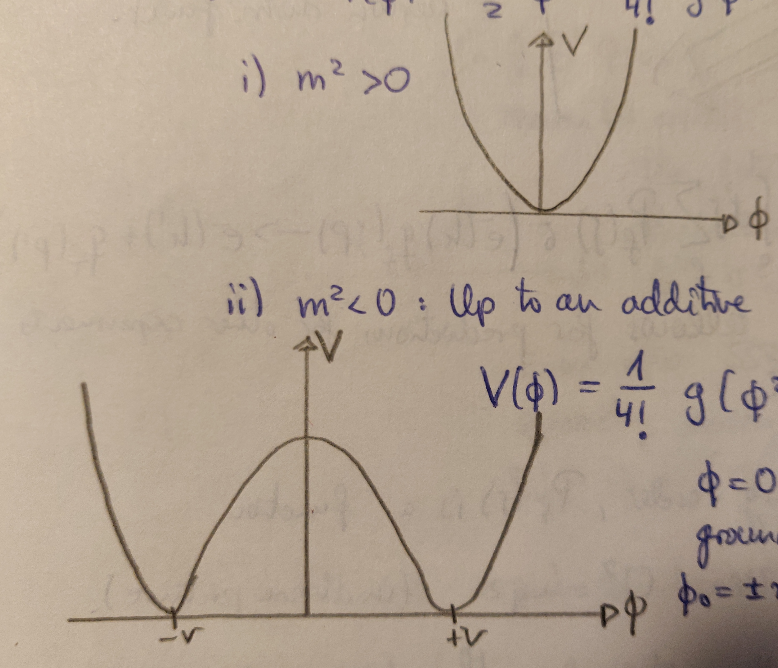
\includegraphics[width=0.7\linewidth]{gfx/YMpictures/SSB}
	\caption{}
	\label{fig:ssb}
\end{figure}
\begin{enumerate}
	\item $m^2>0$, compare \ref{fig:ssb}. We find the classical minimum at $\phi_0=0$ which respects the $\mathbb{Z}_2$ symmetry.
	\item $m^2<0$: Up to an additive constant, we can rewrite the potential as
	\begin{equation}
	V(\phi) = \frac{1}{4!} g(\phi^2- v^2)^2
	\end{equation}
	from which we can read off that $\phi=0$ is not a ground state. The classical ground state at $\phi_0=\pm v$ is degenerate. If $\phi_0=\pm v$, then the symmetry is \emph{broken}.
\end{enumerate}
In QFT, we define the excitations around that vacuum, e.g. $\phi_0=+ v$ by making a mean field approach 
\begin{equation}
	\phi=v+f
\end{equation}
and rewriting $\mL$ as 
\begin{equation}
	\label{eq:ssbLagrangian}
	\mL = \half \partial_\mu f \partial^\mu f - \frac{1}{6} g \left[ v^2 \cdot f^2+ v\cdot f^3 + \frac{1}{4} f^4\right].
\end{equation}
This looks like the theory of a massive scalar $f$ with 
\begin{equation}
	m f^2 = \frac{g}{3} v^3.
\end{equation}
The classical vacuum is at $f=0$ (i.e. at $\phi=v$). \\
\\
We now expand $\hat{f}(x)$ in quantum theory into creation/annihilation modes and  define particles in this way as excitations of $\hat{f}$, i.e. as excitations of $\hat{\phi} = v+ \hat{f}$ around $\expval{\hat{ \phi}}=v$.\\
Note: $f(x)$ has no $\mathbb{Z}_2$-symmetry left, the theory is \emph{spontaneously broken}\footnote{As $\phi\rightarrow -\phi$ corresponds to $v\rightarrow -v$ and $f \rightarrow - f$ and not just a symmetry of $f$ above.}.
\subsection{Continuous symmetries}
For SSb of a continuous, global symmetry a new feature occurs:\\
the existence of massless modes = \emph{Goldstone modes}.\\
\\
Example:\\
Consider a real scalar field $\phi=(\phi_1,\dots,\phi_n)^T$ with $\phi^2 = \phi \circ \phi = \sum_r \phi_r \phi_r$ and
\begin{equation}
\mL = \half \partial^\mu \phi \partial_\mu \phi - V(\phi), \quad V(\phi)= \frac{1}{8} g (\phi^2-v^2)^2, \quad g>0.
\end{equation}
This potential is what people generally (questionable choice of name) call the \emph{Mexican hat potential}, see \ref{fig:mexicanhatpotential}.
\begin{figure}[h!]
	\centering
	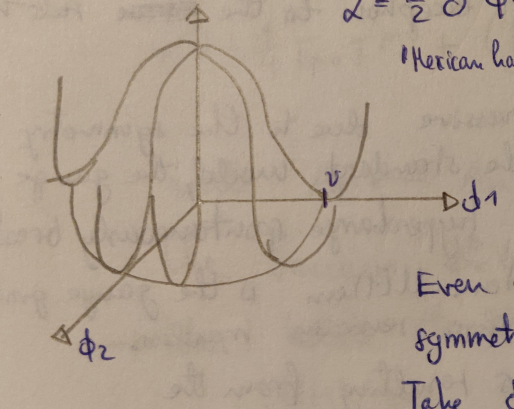
\includegraphics[width=0.7\linewidth]{gfx/YMpictures/MexicanHatPotential}
	\caption{}
	\label{fig:mexicanhatpotential}
\end{figure}
The full symmetry group of $V$ is $G=O(n)$ with the classical ground state being $\phi=\phi_0$ such that $\phi^2_0=v^2$.\\
Even after SSB, i.e. in the vacuum $\phi_0$, there is a residual symmetry corresponding to remaining flat directions:\\
Take $\phi_0=(\underbrace{0,\dots,0}_{(n-1)}, v) \Rightarrow$ $\phi_0$ is invariant under $H=O(n-1)$.\\
\\
Expand $\phi$ about a choice of vacuum $\phi_0$ as above:
\begin{align*}
	\phi&= (\phi_\perp, v+f),\quad \phi_\perp = (\phi_1,\dots,\phi_{n-1}) \\
	V(\phi)&= \frac{g}{2} v^2 f^2 + \frac{g}{2} v (\phi^2_\perp + f^2)f+ \frac{1}{8} g (\phi^2_\perp +f^2)^2.
\end{align*}
From this we can read off
\begin{equation*}
	\begin{array}{ll}
		f \text{ is massive }m^2_f=g v^2 \; &\Rightarrow \; 1 \text{ massive field (e.g. Higgs)}\\
		\phi_\perp \text{ has no mass-term } &\Rightarrow (n-1) \text{ massless fields}\\
	\end{array}
\end{equation*}
The massless fields are called \emph{Goldstone modes} or \emph{Goldstone bosons}.
\subsubsection{What is the idea behind this ?}
We obtain light or massless scalars in the full quantum theory through SSB. The minimum of this potential $V(\phi)$, i.e. the vacuum lies not at the origin but rather degenerates to lie anywhere on the sphere $\mathbb{S}^{n-1}$ defined by $\expval{\phi}=v$. Even if a universe described by such a theory would start at $\phi=0$, quantum fluctuations would quickly destabilize it, leading the whole universe to decay into one of its true  vacuum configurations on $\mathbb{S}^{n-1}$. In that configuration, there would now be one direction in field configuration space, namely the one orthogonal to the sphere, in which the potential $V(\phi)$ has non-zero curvature giving rise to a massive scalar. The Higgs field is an example of this.\\
In all other $n-1$ dimensions, the potential is constant, yielding $n-1$ Goldstone bosons.\\
These Goldstone bosons are massless scalars in the full quantum theory and therefore \textbf{pose an exception to the rule that scalars should be heavy}.
 \paragraph{Example}
The $W^{\pm}$ and $Z^0$ bosons are massive due to the symmetry breaking mechanism. In the SM, the gauge group of the weak force and spontaneously breaks to $SU(2)\times U(1)_Y$$\rightarrow U(1)_{QED}$. $U(1)_{QED}$ is the gauge group of the photon which therefore remains massless. The three Goldstone bosons resulting from the disappearance of $SU(2)$ lend mass to $W^{\pm}$ and $Z^0$.

\subsubsection{The Goldstone Theorem}
For a more in depth treatment look at \ref{subsec:goldstone}.\\
\begin{mybox}{Goldstone's theorem}
	Given a quantum theory with SSB from $G$ to $H$ as above, then there exist 
	\begin{equation*}
		(\dim G-\dim H) \text{ zero mass scalars } = \text{ Goldstone bosons}.
	\end{equation*}
\end{mybox}
Suppose $V$ has global, continuous symmetry $G$ and the vacuum breaks $G\rightarrow H$ spontaneously. Then, the theory after symmetry breaking shows
\begin{equation*}
	(\dim G-\dim H) \text{ massless scalars } = \text{ Goldstone bosons }.
\end{equation*}
\subsection{Goldstone theorem}
\label{subsec:goldstone}
In particle and condensed matter physics, Goldstone bosons or Nambu–Goldstone bosons (NGBs) are bosons that appear necessarily in models exhibiting spontaneous breakdown of continuous symmetries.
\begin{mybox}{Goldstone theorem}
	Goldstone's theorem examines a generic continuous (global) symmetry of the Lagrangian which is spontaneously broken; i.e., its currents are conserved, but the ground state is not invariant under the action of the corresponding charges. Then, necessarily, new massless (or light, if the symmetry is not exact) scalar particles appear in the spectrum of possible excitations. There is one scalar particle—called a Nambu–Goldstone boson—for each generator of the symmetry that is broken, i.e., that does not preserve the ground state. The Nambu–Goldstone mode is a long-wavelength fluctuation of the corresponding order parameter.\\
	In theories with gauge symmetry, i.e. with local continuous symmetries, the Goldstone bosons are "eaten" by the gauge bosons. The latter become massive and their new, longitudinal polarization is provided by the Goldstone boson.
\end{mybox}
Some intuition why the Goldstone boson should be massless in the case of explicit calculation of spontaneous symmetry breaking ;\\
If you split the potential into contributions from real fields $\phi_1$, $\phi_2$, we observe that the minima of the potential make up a circle in the $(\phi_1,\phi_2)$-plane. However, the potential only increases in $\phi_1$ direction, therefore moving a bit in $\phi_2$ direction does not require any energy to climb up the potential for the fluctuations to take place, therefore $m_{\rho_2}=0$ and we only find massless modes in this field-axis.\\

\subsubsection{Explicit calculation}
Consider a complex scalar field $\phi$, with the constraint that $\phi^* \phi=v^2$, a constant. One way to impose a constraint of this sort is by including a potential interaction term in its Lagrangian density,
\begin{equation}
V(\phi) = \lambda (\phi^* \phi - v^2)^2,
\end{equation}
and taking the limit as $\lambda \rightarrow \infty$  (this is called the "\emph{Abelian nonlinear $\sigma$-model}". It corresponds to the Goldstone sombrero potential where the tip and the sides shoot to infinity, preserving the location of the minimum at its base).\\
The constraint, and the action, below, are invariant under a $U(1)$ phase transformation, $\delta \phi = i \epsilon \phi$. The field can be redefined to give a real scalar field (i.e., a spin-zero particle) $\theta$ without any constraint by
\begin{equation}
\phi = v e^{i \theta}
\end{equation}
where $\theta$ is the Nambu–Goldstone boson (actually $v\theta$ is), and the $U(1)$ symmetry transformation effects a shift on $\theta$, namely
\begin{equation}
\delta \theta = \epsilon
\end{equation}
but does not preserve the ground state $\ket{0}$ (i.e. the above infinitesimal transformation does not annihilate it—the hallmark of invariance), as evident in the charge of the current below.\\
Thus, the vacuum is degenerate and noninvariant under the action of the spontaneously broken symmetry.\\
The corresponding Lagrangian density is given by
\begin{equation}
\mL =- \half \partial^\mu \phi^* \partial_\mu \phi + m^2 \phi^* \phi = -\half \left(-i ve^{-i \theta} \partial^\mu \theta\right)\left(ive^{i\theta} \partial_\mu \theta\right) + m^2 v^2
\end{equation}
and thus
\begin{equation}
= -\frac{v^2}{2} \partial^\mu \theta\partial_\mu\theta + m^2 v^2.
\end{equation}
Note that the constant term $m^2v^2$ in the Lagrangian density has no physical significance, and the other term in it is simply the kinetic term for a massless scalar.
\\
The symmetry-induced conserved $U(1)$ current is
\begin{equation}
J_\mu = -v^2 \partial_\mu \theta.
\end{equation}
The charge, $Q$, resulting from this current shifts $\theta$ and the ground state to a new, degenerate, ground state. Thus, a vacuum with $\expval{\theta}=0$ will shift to a different vacuum with $\expval{\theta}=-\epsilon$. The current connects the original vacuum with the Nambu–Goldstone boson state, $\expval{J_0(0)}{0} \neq 0$.\\
In general, in a theory with several scalar fields, $\phi_j$, the Nambu–Goldstone mode $\phi_g$ is massless, and parameterises the curve of possible (degenerate) vacuum states. Its hallmark under the broken symmetry transformation is nonvanishing vacuum expectation $\expval{\delta \phi_g}$, an order parameter, for vanishing $\expval{\phi_g}=0$, at some ground state $\ket{0}$ chosen at the minimum of the potential, $\expval{\frac{\partial V}{\partial \phi_i}}=0$. Symmetry dictates that all variations of the potential with respect to the fields in all symmetry directions vanish. The vacuum value of the first order variation in any direction vanishes as just seen; while the vacuum value of the second order variation must also vanish, as follows. Vanishing vacuum values of field symmetry transformation increments add no new information.\\
By contrast, however, nonvanishing vacuum expectations of transformation increments, $\expval{\delta \phi_g}$, specify the relevant (Goldstone) null eigenvectors of the mass matrix,
\begin{equation}
\expval{\frac{\partial^2 V}{\partial \phi_i \partial_j}} \expval{\delta \phi_g} =0
\end{equation}
and hence the corresponding zero-mass eigenvalues.
\subsubsection{Goldstone's argument}
The principle behind Goldstone's argument is that the ground state is not unique. Normally, by current conservation, the charge operator for any symmetry current is time-independent,
\begin{equation}
\frac{\md Q}{\md t} = \int \md x J^0(x) = 0.
\end{equation}
Acting with the charge operator on the vacuum either annihilates the vacuum, if that is symmetric; else, if not, as is the case in spontaneous symmetry breaking, it produces a zero-frequency state out of it, through its shift transformation feature illustrated above. Actually, here, the charge itself is ill-defined, cf. the Fabri–Picasso argument below.\\
But its better behaved commutators with fields, that is, the nonvanishing transformation shifts $\expval{\delta \phi_g}$, are, nevertheless, time-invariant,
\begin{equation}
\frac{\md \expval{\delta \phi_g}}{\md t} = 0
\end{equation}
thus generating a $\delta(k^0)$ in its Fourier transform. (This ensures that, inserting a complete set of intermediate states in a nonvanishing current commutator can lead to vanishing time-evolution only when one or more of these states is massless.)\\
Thus, if the vacuum is not invariant under the symmetry, action of the charge operator produces a state which is different from the vacuum chosen, but which has zero frequency. This is a long-wavelength oscillation of a field which is nearly stationary: there are physical states with zero frequency, $k^0$, so that the theory \textbf{cannot have a mass gap}. However this argument fails when the symmetry is gauged, because then the symmetry generator is only performing a gauge transformation. A gauge transformed state is the same exact state, so that acting with a symmetry generator does not get one out of the vacuum.
\subsubsection{Non-relativistic theories}
A version of Goldstone's theorem also applies to nonrelativistic theories (and also relativistic theories with spontaneously broken spacetime symmetries, such as Lorentz symmetry or conformal symmetry, rotational, or translational invariance).\\
It essentially states that, for each spontaneously broken symmetry, there corresponds some quasiparticle with no energy gap—the nonrelativistic version of the mass gap. (Note that the energy here is really $H−\mu N−\vec{\alpha}\cdot \vec{P}$ and not $H$.) However, two different spontaneously broken generators may now give rise to the same Nambu–Goldstone boson. For example, in a superfluid, both the $U(1)$ particle number symmetry and Galilean symmetry are spontaneously broken. However, the phonon is the Goldstone boson for both.\\
In general, the phonon is effectively the Nambu–Goldstone boson for spontaneously broken Galilean/Lorentz symmetry. However, in contrast to the case of internal symmetry breaking, when spacetime symmetries are broken, the order parameter need not be a scalar field, but may be a tensor field, and the corresponding independent massless modes may now be fewer than the number of spontaneously broken generators, because the Goldstone modes may now be linearly dependent among themselves: e.g., the Goldstone modes for some generators might be expressed as gradients of Goldstone modes for other broken generators.
\subsubsection{Pseudo-Goldstone bosons}
Pseudo-Goldstone bosons arise in a quantum field theory with both spontaneous and explicit symmetry breaking. These two types of symmetry breaking typically occur separately, and at different energy scales, and are not thought to be predicated on each other.
In the absence of explicit breaking, spontaneous symmetry breaking would engender massless Nambu–Goldstone bosons for the exact spontaneously broken chiral symmetries. The chiral symmetries discussed, however, are only approximate symmetries, given their small explicit breaking.
\\
The explicit symmetry breaking occurs at a smaller energy scale. The properties of these pseudo-Goldstone bosons can normally be calculated using chiral perturbation theory, expanding around the exactly symmetric theory in terms of the explicit symmetry-breaking parameters. In particular, the computed mass must be small,$m_\pi \approx \sqrt{v m_q}/f_\pi$.

\subsection{Explicit calculation of the SSB mechanism }
\subsubsection{SM course}
We begin by picking a vacuum state $\expval{\phi} = \frac{v}{\sqrt{2}}$ for $V(\phi) = \lambda (\abs{\phi}^2- \half v^2)^2$. Then we do a mean-field decomposition
\begin{equation}
	\phi(x) = \expval{\phi} + \rho(x), \quad \expval{\rho(x)}=0
\end{equation}
and substitute this into $\mL$. The $\rho(x)$ fluctuations now lead to elementary particles, i.e. think of a harmonic oscillator parabola opened upwards with ground-state being centred in the origin, then the fluctuations are the first states appearing above mass gap as states oscillating from one side of the potential to the other.Substituting and decomposing
\begin{equation}
	\rho(x) = \frac{1}{\sqrt{2}} \left[\rho_1(x) + i \rho_2(x)\right]
\end{equation}
yields a Lagrangian with interaction terms implying the following physical characteristica of the theory
\begin{enumerate}
	\item $\lambda v^2 \rho^2_1 \equiv \half m^2_{\rho_1}$
	\item $0 \cdot \rho^2_2 \Rightarrow m_{\rho_2}=0$
	\item Interactions as $\rho^3_1$ vertex, $\rho^4_2$ vertex and a $\rho_2 \rho^2_1$ vertex.
\end{enumerate}
We have broken the symmetry spontaneously and found one massless particle $\rho_2$, this is the Goldstone Boson. See further later.
\subsection{Spontaneous symmetry breaking in physics - Examples}
Examples are
\begin{enumerate}
\item 	For ferromagnetic materials, the underlying laws are invariant under spatial rotations. Here, the order parameter is the magnetization, which measures the magnetic dipole density. Above the Curie temperature, the order parameter is zero, which is spatially invariant, and there is no symmetry breaking. Below the Curie temperature, however, the magnetization acquires a constant nonvanishing value, which points in a certain direction (in the idealized situation where we have full equilibrium; otherwise, translational symmetry gets broken as well). The residual rotational symmetries which leave the orientation of this vector invariant remain unbroken, unlike the other rotations which do not and are thus spontaneously broken.
	 \item The laws describing a solid are invariant under the full Euclidean group, but the solid itself spontaneously breaks this group down to a space group. The displacement and the orientation are the order parameters.
	\item General relativity has a Lorentz symmetry, but in FRW cosmological models, the mean 4-velocity field defined by averaging over the velocities of the galaxies (the galaxies act like gas particles at cosmological scales) acts as an order parameter breaking this symmetry. Similar comments can be made about the cosmic microwave background.
	\item For the electroweak model, as explained earlier, a component of the Higgs field provides the order parameter breaking the electroweak gauge symmetry to the electromagnetic gauge symmetry. Like the ferromagnetic example, there is a phase transition at the electroweak temperature. The same comment about us not tending to notice broken symmetries suggests why it took so long for us to discover electroweak unification.
	\item In superconductors, there is a condensed-matter collective field ψ, which acts as the order parameter breaking the electromagnetic gauge symmetry.
	\item Take a thin cylindrical plastic rod and push both ends together. Before buckling, the system is symmetric under rotation, and so visibly cylindrically symmetric. But after buckling, it looks different, and asymmetric. Nevertheless, features of the cylindrical symmetry are still there: ignoring friction, it would take no force to freely spin the rod around, displacing the ground state in time, and amounting to an oscillation of vanishing frequency, unlike the radial oscillations in the direction of the buckle. This spinning mode is effectively the requisite Nambu–Goldstone boson.
	\item Consider a uniform layer of fluid over an infinite horizontal plane. This system has all the symmetries of the Euclidean plane. But now heat the bottom surface uniformly so that it becomes much hotter than the upper surface. When the temperature gradient becomes large enough, convection cells will form, breaking the Euclidean symmetry.
	\item Consider a bead on a circular hoop that is rotated about a vertical diameter. As the rotational velocity is increased gradually from rest, the bead will initially stay at its initial equilibrium point at the bottom of the hoop (intuitively stable, lowest gravitational potential). At a certain critical rotational velocity, this point will become unstable and the bead will jump to one of two other newly created equilibria, equidistant from the center. Initially, the system is symmetric with respect to the diameter, yet after passing the critical velocity, the bead ends up in one of the two new equilibrium points, thus breaking the symmetry.
\end{enumerate}
\subsubsection{Particle physics}
In particle physics the force carrier particles are normally specified by field equations with gauge symmetry; their equations predict that certain measurements will be the same at any point in the field. For instance, field equations might predict that the mass of two quarks is constant. Solving the equations to find the mass of each quark might give two solutions. In one solution, quark $A$ is heavier than quark $B$. In the second solution, quark $B$ is heavier than quark $A$ by the same amount. The symmetry of the equations is not reflected by the individual solutions, but it is reflected by the range of solutions.\\
An actual measurement reflects only one solution, representing a breakdown in the symmetry of the underlying theory. "Hidden" is a better term than "broken", because the symmetry is always there in these equations. This phenomenon is called spontaneous symmetry breaking (SSB) because nothing (that we know of) breaks the symmetry in the equations
\subsubsection{Chiral symmetry}
\todo{Expand }
\label{subsubsec:chiralsymmetry}
\emph{Chiral Symmetry}:\\




\emph{Chiral Symmetry Breaking}:\\
In particle physics, chiral symmetry breaking is the spontaneous symmetry breaking of a chiral symmetry – usually by a gauge theory such as quantum chromodynamics, the quantum field theory of the strong interaction.\\
Chiral symmetry breaking is an example of spontaneous symmetry breaking affecting the chiral symmetry of the strong interactions in particle physics. It is a property of QCD and thus of all common matter, as it converts very light bound quarks into $100$ times heavier constituents of baryons. The approximate Nambu–Goldstone bosons in this spontaneous symmetry breaking process are the pions, whose mass is an order of magnitude lighter than the mass of the nucleons. It served as the prototype and significant ingredient of the Higgs mechanism underlying the electroweak symmetry breaking.
























\subsection{Higgs mechanism}
\label{subsec:higgs}
The strong, weak, and electromagnetic forces can all be understood as arising from gauge symmetries. The Higgs mechanism, the spontaneous symmetry breaking of gauge symmetries, is an important component in understanding the superconductivity of metals and the origin of particle masses in the standard model of particle physics. One important consequence of the distinction between true symmetries and gauge symmetries, is that the spontaneous breaking of a gauge symmetry does not give rise to characteristic massless Nambu–Goldstone physical modes, but only massive modes, like the plasma mode in a superconductor, or the Higgs mode observed in particle physics.\\
In the standard model of particle physics, spontaneous symmetry breaking of the $SU(2) \times U(1)$ gauge symmetry associated with the electro-weak force generates masses for several particles, and separates the electromagnetic and weak forces. The $W$ and $Z$ bosons are the elementary particles that mediate the weak interaction, while the photon mediates the electromagnetic interaction. At energies much greater than $100$ GeV all these particles behave in a similar manner. The Weinberg–Salam theory predicts that, at lower energies, this symmetry is broken so that the photon and the massive $W$ and $Z$ bosons emerge. In addition, fermions develop mass consistently.\\
Without spontaneous symmetry breaking, the Standard Model of elementary particle interactions requires the existence of a number of particles. However, some particles (the $W$ and $Z$ bosons) would then be predicted to be massless, when, in reality, they are observed to have mass. To overcome this, spontaneous symmetry breaking is augmented by the Higgs mechanism to give these particles mass. It also suggests the presence of a new particle, the Higgs boson, detected in $2012$.\\
Superconductivity of metals is a condensed-matter analogue of the Higgs phenomena, in which a condensate of Cooper pairs of electrons spontaneously breaks the $U(1)$ gauge symmetry associated with light and electromagnetism.
\subsubsection{Condensed matter physics}
Most phases of matter can be understood through the lens of spontaneous symmetry breaking. For example, crystals are periodic arrays of atoms that are not invariant under all translations (only under a small subset of translations by a lattice vector). Magnets have north and south poles that are oriented in a specific direction, breaking rotational symmetry. In addition to these examples, there are a whole host of other symmetry-breaking phases of matter including nematic phases of liquid crystals, charge- and spin-density waves, superfluids and many others.\\
There are several known examples of matter that cannot be described by spontaneous symmetry breaking, including: topologically ordered phases of matter like fractional quantum Hall liquids, and spin-liquids. These states do not break any symmetry, but are distinct phases of matter. Unlike the case of spontaneous symmetry breaking, there is not a general framework for describing such states.


\subsubsection{Continuous symmetry}
The ferromagnet is the canonical system which spontaneously breaks the continuous symmetry of the spins below the Curie temperature and at $h = 0$, where $h$ is the external magnetic field. Below the Curie temperature the energy of the system is invariant under inversion of the magnetization $m(x)$ such that $m(x) = −m(−x)$. The symmetry is spontaneously broken as $h \rightarrow 0$ when the Hamiltonian becomes invariant under the inversion transformation, but the expectation value is not invariant.\\
Spontaneously-symmetry-broken phases of matter are characterized by an \emph{order parameter} \todo{Look into this, Landau theory ?} that describes the quantity which breaks the symmetry under consideration. For example, in a magnet, the order parameter is the local magnetization.\\
Spontaneously breaking of a continuous symmetry is inevitably accompanied by gapless (meaning that these modes do not cost any energy to excite) Nambu–Goldstone modes associated with slow long-wavelength fluctuations of the order parameter. For example, vibrational modes in a crystal, known as phonons, are associated with slow density fluctuations of the crystal's atoms. The associated Goldstone mode for magnets are oscillating waves of spin known as spin-waves. For symmetry-breaking states, whose order parameter is not a conserved quantity, Nambu–Goldstone modes are typically massless and propagate at a constant velocity.\\
An important theorem, due to Mermin and Wagner \ref{subsubsec:merminwagnertheorem}, states that, at finite temperature, thermally activated fluctuations of Nambu–Goldstone modes destroy the long-range order, and prevent spontaneous symmetry breaking in one- and two-dimensional systems. Similarly, quantum fluctuations of the order parameter prevent most types of continuous symmetry breaking in one-dimensional systems even at zero temperature (an important exception is ferromagnets, whose order parameter, magnetization, is an exactly conserved quantity and does not have any quantum fluctuations).\\
Other long-range interacting systems such as cylindrical curved surfaces interacting via the Coulomb potential or Yukawa potential has been shown to break translational and rotational symmetries. It was shown, in the presence of a symmetric Hamiltonian, and in the limit of infinite volume, the system spontaneously adopts a chiral configuration, i.e. breaks mirror plane symmetry.
\subsubsection{Dynamical symmetry breaking}
\textbf{Dynamical symmetry breaking (DSB) is a special form of spontaneous symmetry breaking where the ground state of the system has reduced symmetry properties compared to its theoretical description (Lagrangian). Dynamical breaking of a global symmetry is a spontaneous symmetry breaking, that happens not at the (classical) tree level (i.e. at the level of the bare action), but due to quantum corrections (i.e. at the level of the effective action)}.\\
Dynamical breaking of a gauge symmetry is subtler. In the conventional spontaneous gauge symmetry breaking, there exists an unstable Higgs particle in the theory, which drives the vacuum to a symmetry-broken phase (see e.g. Electroweak interaction). In dynamical gauge symmetry breaking, however, no unstable Higgs particle operates in the theory, but the bound states of the system itself provide the unstable fields that render the phase transition. For example, Bardeen, Hill, and Lindner published a paper which attempts to replace the conventional Higgs mechanism in the standard model by a DSB that is driven by a bound state of top-antitop quarks (such models, where a composite particle plays the role of the Higgs boson, are often referred to as "Composite Higgs models"). Dynamical breaking of gauge symmetries is often due to creation of a fermionic condensate; for example the quark condensate, which is connected to the dynamical breaking of chiral symmetry in quantum chromodynamics. Conventional superconductivity is the paradigmatic example from the condensed matter side, where phonon-mediated attractions lead electrons to become bound in pairs and then condense, thereby breaking the electromagnetic gauge symmetry.
\subsubsection{Generalization and technical usage}
For spontaneous symmetry breaking to occur, there must be a system in which there are several equally likely outcomes. The system as a whole is therefore symmetric with respect to these outcomes. However, if the system is sampled (i.e. if the system is actually used or interacted with in any way), a specific outcome must occur. Though the system as a whole is symmetric, it is never encountered with this symmetry, but only in one specific asymmetric state. Hence, the symmetry is said to be spontaneously broken in that theory. Nevertheless, the fact that each outcome is equally likely is a reflection of the underlying symmetry, which is thus often dubbed "hidden symmetry", and has crucial formal consequences (see Goldstone boson\ref{subsec:goldstone}).\\
When a theory is symmetric with respect to a symmetry group, but requires that one element of the group be distinct, then spontaneous symmetry breaking has occurred. The theory must not dictate which member is distinct, only that one is. From this point on, the theory can be treated as if this element actually is distinct, with the proviso that any results found in this way must be resymmetrized, by taking the average of each of the elements of the group being the distinct one.
\\
The crucial concept in physics theories is the \emph{order parameter}. If there is a field (often a background field) which acquires an expectation value (not necessarily a vacuum expectation value) which is not invariant under the symmetry in question, we say that the system is in the ordered phase, and the symmetry is spontaneously broken. This is because other subsystems interact with the order parameter, which specifies a "frame of reference" to be measured against. In that case, the vacuum state does not obey the initial symmetry (which would keep it invariant, in the linearly realized Wigner mode in which it would be a singlet), and, instead changes under the (hidden) symmetry, now implemented in the (non-linear) Nambu–Goldstone mode. Normally, in the absence of the Higgs mechanism, massless Goldstone bosons arise.\\
\todo{Think in general about background field method, also in context of 1PI, and order parameter.}
The symmetry group can be discrete, such as the space group of a crystal, or continuous (e.g., a Lie group), such as the rotational symmetry of space. However, if the system contains only a single spatial dimension, then only discrete symmetries may be broken in a vacuum state of the full quantum theory, although a classical solution may break a continuous symmetry.

\subsubsection{The Higgs mechanism - Weigand}
\label{subsubsec:higgsWeigand}
Consider a gauge theory with SSB from a
\begin{equation}
	\text{gauged } G \longrightarrow \text{gauged }H.
\end{equation}
\begin{mybox}{The Higgs mechanism in essence}
The Higgs effect is the phenomenon that the $\dim G -\dim H$ Goldstone bosons are "eaten", i.e. absorbed by $\dim G-\dim H$ vector bosons, which thereby become massive. I.e. the "would-be" Goldstone bosons constitute the third, longitudinal d.o.f. of the massive gauge bosons
\begin{equation*}
	A^{\hat{a}}_\mu \quad \hat{a}=\dim H+1,\dots,\dim G.
\end{equation*}
$H$ relies on the local character of the gauge symmetry group $G$ (and H). Goldstone modes are associated with the transformations $T^{\hat{a}}$ that \textbf{do not leave the vacuum invariant}. These can be gauged away if $G$ is local- for global $G$ it is not possible since a particle is a local excitation.
\end{mybox}
Consider a $U(1)$ gauge theory with complex boson $\Phi$ 
\begin{equation*}
	\mL = - \frac{1}{4} F\munu F^{\mu \nu} + (\underbrace{D_\mu \phi}_{\partial_\mu \phi -i e A_\mu \phi})^\dagger (D^\mu \phi) - \underbrace{V(\phi^*  \phi)}_{\frac{g}{2} (\phi^* \phi- \frac{v^2}{2})^2}
\end{equation*}
with
\begin{equation}
A_\mu \rightarrow A_\mu + \frac{1}{e} \partial_\mu \chi(x) \quad \text{and} \quad \phi\rightarrow e^{i\chi(x)} \phi
\end{equation}
a local $U(1)$ gauge trafo. The vacuum $\phi^* \phi = \frac{v^2}{2}$ breaks the $U(1)$ symmetry.\\
\\
Idea:
\\
Isolate the Goldstone mode corresponding to the broken $U(1)$ trafo by choosing the parametrization
\begin{equation}
	\label{eq:higgsparametrization}
	\phi(x)= \frac{1}{\sqrt{2} } \left[v+f(x)\right] e^{-i \frac{\theta(x)}{v}} \; \& \; A_\mu(x) := B_\mu - \frac{1}{3} \frac{\partial_\mu \theta(x)}{v},
\end{equation}
where $f(x)$ is the Higgs scalar and $\theta(x)$ corresponds to the $U(1)$ trafo and therefore will be the resulting Goldstone boson. Then, we find
\begin{align*}
	D_\mu \phi &= \frac{1}{\sqrt{2}} e^{-\frac{\theta(x)}{v}} \left[\partial_\mu f- ieB_\mu (v+f)\right]\\
	\Rightarrow \; \mL &= - \frac{1}{4} F\munu F^{\mu \nu} + \half e^2 (v+f)^2 B_\mu B^\mu + \half \partial_\mu f \partial^\mu f - \frac{1}{8} g (2 v f+f^2)^2.
\end{align*}
From this we can read off the following properties
\begin{enumerate}
\item $f$ is a massive scalar: $mf^2 = gv^2$.
\item $B^\mu$ is a \emph{massive} vector field $m^2_B = e^2 v^2$.
\item No massless scalar is left !
\end{enumerate}
\paragraph{Reason}
The $U(1)$ boson has absorbed the would-be Goldstone mode $\theta(x)$.
\paragraph{Note}
The Goldstone mode can be gauge away by going to unitarity gauge, which is a gauge in which the Lagrangian only contains physical degrees of freedom:
\begin{equation}
\phi \rightarrow \frac{1}{\sqrt{2}} (v+f(x)) \; \& \; A_\mu \rightarrow B_\mu \quad \Rightarrow \phi=\phi^*.
\end{equation}
\subsubsection{Note on Higgs in SM}
In the SM, at temperatures high enough that the electroweak symmetry is unbroken, all elementary particles are massless. At a critical temperature, the Higgs field becomes tachyonic (which is a field with imaginary mass, i.e. $m^2<0$); the symmetry is spontaneously broken by condensation, and the $W$ and $Z$ bosons acquire masses, this is called \emph{electroweak symmetry breaking}.\\
The photon and $Z$ boson are formed by the mixing resulting from the Higgs mechanism.\\
This is developed more in-depth below \ref{subsubsec:higgsSMSSB}.

\subsubsection{Abelian Higgs Model - an explicit calculation}
The Higgs mechanism is spontaneous symmetry breaking explicitly for the case of a gauge theory, consider here an abelian gauge theory 
\begin{equation}
\mL = (\partial_\mu \phi^*) \partial^\mu \phi - \lambda (\phi^* \phi - \half v^2)^2
\end{equation}
and make it $U(1)$ gauge invariant via the minimal coupling scheme
\begin{align}
	\phi(x) & \rightarrow U(x) \phi(x), \; \phi^*(x) \rightarrow \phi^*(x) U^\dagger(x),\\
	A_\mu(x) &\rightarrow A_\mu(x) + \frac{1}{e} \partial_\mu \alpha(x), \quad U(x)=e^{.i\alpha(x)} \in U(1)\\
	\Rightarrow\quad \mL &\rightarrow\mL = -\frac{1}{4} F\munu F^{\mu \nu} + (D_\mu \phi)^* (D^\mu \phi) - \underbrace{\lambda(\abs{\phi}^2-\half v^2)^2}_{V(\phi,\phi^*)} 
\end{align}
the abelian Higgs model.\\
This $U(1)$ gauge symmetry is now spontaneously broken as the non-vanishing VEV singles out a particular vacuum state
\begin{equation}
\expval{\phi}=\frac{v}{\sqrt{2}} \;\Rightarrow \; \expval{\phi}\rightarrow e^{-i\alpha(x)} \expval{\phi}\neq \frac{v}{\sqrt{2}} \text{ no invariance}.
\end{equation}
The difference to the spontaneous breaking of global symmetries arises now in the following. We again have to redefine the field variables
\begin{equation}
\phi(x) = \frac{1}{\sqrt{2}} \left[v+\rho(x)\right] e^{i \xi(x)}, \; \rho,\xi \in \mR, \; \expval{\rho} = \expval{\xi} =0,
\end{equation}
which is a different decomposition to the global SSB but we still have only $2$ real degrees of freedom. Now we fix the gauge to unitary gauge $\alpha(x) =\xi(x)$ (which is a good gauge choice if you want to identify physical degrees of freedom):
\begin{equation}
\phi(x) \rightarrow\phi(x) e^{-i\alpha(x)} \equiv \phi(x) e^{-i\xi(x)} = \frac{1}{\sqrt{2}} [v+\rho(x)]
\end{equation}
\begin{mybox}{Remark on gauge-invariance and anomalies}
	If you are not calculating on a lattice, the gauge always has to be fixed. At intermediate stages of the calculation results will therefore be gauge-dependent. How do we know that gauge-invariance is restored at end of calculation ? If it is not, then we have a \textbf{gauge anomaly} (by UV regularization cut-off), the theory is then dead. If we have a \emph{global anomaly}, the theory will still work, but the symmetry objects (Noether current) are just badly chosen. So, how do we then know that it will be gauge-invariant at the end ? The Ward identities are the answer. Note that in the abelian gauge theories we have Ward-Takahashi identities whilst in the non-abelian case we have Slavnov-Taylor identities, where for the latter we have to do BRST trafo to guarantee gauge-invariance in the end.
\end{mybox}
\todo{Look into anomalies, Ward identities and link to original chapter.}
Now expand $\mL$ in the unitary gauge and look for a mass term. Schematically we find terms of the form
\begin{enumerate}
	\item \begin{equation}
	\frac{e^2 v^2}{2} A^\mu A_\mu \quad \Rightarrow \quad m_A =ev\neq 0
	\end{equation}
	the gauge field therefore becomes massive due to the non-vanishing VEV.
	\item \begin{equation}
	-\frac{\lambda}{4} (2 \rho v + \rho)^2 \quad \Rightarrow \quad  m_\rho = \sqrt{2 \lambda} v \neq 0.
	\end{equation}
\end{enumerate}
Gauge invariance is spontaneously broken such that the gauge boson is massive now. How ? Count the real degrees of freedom.
Before SSB and gauge fixing we had $2$ fields:
\begin{align*}
	A_\mu& \text{ massless vector field with }2 \text{ real dof, the two transverse pol.}\\
	\phi \in \mathbb{C}& \; 2\; \text{real dof.} \quad \Rightarrow 4 \text{ real dof.}
\end{align*}
but after SSB and gauge fixing we have
\begin{align*}
	A_\mu& \text{ massive, thus }3\text{ physical dof, two transv. and one long. pol.}\\
	\phi& 1 \text{ real dof}=\rho(x) \text{ physical Higgs boson} \Rightarrow\; 4 dof.
\end{align*}
The dof $\rho(x)$ which we gauged away is called the unrealized Goldstone boson, it gave rise to the longitudinal polarization of $A_\mu$.\footnote{Apparently this is called G}
\begin{mybox}{Goldstone equivalence theorem}
	This comprises the Goldstone equivalence theorem. In the Higgs mechanism, a massive W boson acquired its
	longitudinal component by absorbing a Goldstone boson from the Higgs sector. 
\end{mybox}
Summarizing the Higgs mechanism:\\
For SSB of gauge symmetry, for every broken generator of the gauge group the corresponding vector boson becomes massive. This massive $A_\mu$ has $3$ polarizations ($+,-,L$), $L$ corresponds to the unrealized Goldstone boson. The remaining part of the scalar field is the physical massive Higgs boson $\rho$.\footnote{The mass will always be proportional to the coupling and the VEV.}

\subsubsection{Higgs SSB of electroweak sector in the SM}
\label{subsubsec:higgsSMSSB}
How does the SSB of $SU(2)_L \times U(1)_Y$ $\rightarrow U(1)_{QED}$ work ?\\
Note that we choose $\expval{H}= \frac{1}{\sqrt{2}} (0,v)^T$ such that we have
\begin{equation}
\expval{H} \stackrel{SU(2)_L \times U(1)_Y}{\longrightarrow} \exp\left[-i \alpha^a(x) \underbrace{T^a_{SU(2)_L}}_{\frac{\sigma^a}{2}} -i \beta(x) \underbrace{y}_{=\half} \mI_2 \right] \expval{H}.
\end{equation}
Which of the $4$ generators $T^{1,2,3}, y\mI_2$ of the electro-weak sector does $v\neq 0$ break ?\\
We fix the $SU(2)_L$ gauge as follows
\begin{equation}
\alpha^1(x) =0=\alpha^2(x), \alpha^3(x) = \beta(x),
\end{equation}
such that the VEV becomes invariant under $SU(2)_L\times U(1)_Y$ trafo \emph{by our choice} of $\expval{H}$
\begin{equation}
\exp\left[-i \beta(x) \begin{pmatrix}
\half & 0 \\
0 & - \half \\
\end{pmatrix}
-i \beta(x) 
\begin{pmatrix}
\half &0 \\
0& \half \\
\end{pmatrix}
\right]
\begin{pmatrix}
0 \\
\frac{v}{\sqrt{2}}
\end{pmatrix}
= \exp\left[-\beta(x) \begin{pmatrix}
1&0 \\
0&0 \\
\end{pmatrix}\right] \begin{pmatrix}
0 \\
\frac{v}{\sqrt{2}}
\end{pmatrix}
= \begin{pmatrix}
0 \\
\frac{v}{\sqrt{2}}\\
\end{pmatrix} = \expval{H}.
\end{equation}
Therefore, it is exactly this generator
\begin{equation}
T^3+y\mI=\begin{pmatrix}
1 & 0 \\
0 & 0 \\
\end{pmatrix}\stackrel{\ref{eq:electricchargeSM}}{=} Q_e
\end{equation}
which is unbroken, where all others (meaning all other linear combinations of our $4$ operators) are broken. This generator will then be the generator of $U(1)_{QED}$, i.e. $Q_e$ (where this representation is of course only valid for this particular Higgs doublet). There is thus only one linear combination (up to $\gamma \in \mR_{>0}$) which survives, namely $Q_e$. This is where the sum rule \ref{eq:electricchargeSM} actually comes from, by requiring that the unbroken generator be associated with $Q_e$. \todo{Compare Peskin Schröder Chapter 20.2 onwards !}
\subsubsection{Higgs mechanism for fermions}

The Higgs mechanism can also be used to include the masses of fermions in the SM. We consider a Dirac fermion and require it to transform differently under $U(1)$, i.e.
\begin{equation}
\psi_L \rightarrow e^{-i\alpha(x)} \psi_L, \quad \psi_R\rightarrow \psi_R singlet.
\end{equation}

We can not simply add a mass term to the Lagrangian as it would couple LH and RH sector, which would break invariance as they transform differently under the gauge transformation. 
\begin{enumerate} 
	\item How to include quark masses:\\
	Include masses via Yukawa coupling to a scalar Higgs field
	\begin{equation}
	\mL + \bar{ \psi}_L i \slashed{D} \psi_L + \bar{\psi}_R i \slashed{\partial} \psi_R + Y \bar{\psi}_R \phi^\dagger \psi_L.
	\end{equation}
	Decomposing the Higgs, it will now give rise to the masses of everything it couples to
	\begin{equation}
	\phi=\frac{v}{\sqrt{2}}+\rho(x) \; \frac{Y v}{\sqrt{2}} \bar{ \psi}_R \psi_L + \frac{Y^* v}{\sqrt{2}} \bar{ \psi}_L \psi_R \in \mL\; \Rightarrow m_\psi \neq 0.
	\end{equation}
	More in depth, we include Yukawa interactions of the form 
	\begin{align}
		\mL^{\text{quark}}_{\text{Yukawa interaction}} &= -y_{d} \underbrace{\underbrace{\overbrace{\bar{Q}_L H d_R}^{\bar{\mathbf{3}} \mathbf{1} \mathbf{3} =\bar{\mathbf{3}} \mathbf{3}=\mathbf{1}\text{ singlet for } SU(3)_C }}_{\bar{\mathbf{2}} \mathbf{2} \mathbf{1}=\mathbf{1} \mathbf{1} \text{ singlet for } SU(2)_L}}_{-\frac{1}{6} -\frac{1}{3}+\half =0 \text{ singlet for } U(1)_Y} \\
		&- y_u \epsilon^{ab}\underbrace{\underbrace{\overbrace{ (\bar{Q})_a (H^\dagger)_b u_R}^{\bar{\mathbf{3}} \mathbf{1} \mathbf{3} = \mathbf{1} \text{ singlet for } SU(3)_C} }_{\epsilon\bar{\mathbf{2}} \bar{\mathbf{2}} \mathbf{1} = \mathbf{2} \bar{\mathbf{2}} \mathbf{1}=\mathbf{1} \text{ singlet for } SU(2)_L }}_{-\frac{1}{6}+ ?-\frac{2}{3} = 0 \text{ singlet for } U(1)_Y} \nonumber
	\end{align}
	\footnote{Note that only in $SU(2)_L$ you can turn an antifund. into a fund. via the $\epsilon$ tensor, as you have relationship \ref{eq:fundamentalAntifundamentalreprelation} being trivial as $N-1=1$. Doesn't work for $SU(3)$ as $3$ indices.} 
	Note that this is completely gauge-invariant as both are singlets under the whole SM gauge group, as calculated in the term explicitly. The Yukawa coupling constants $y_{d},y_u$ are dimensionless, therefore this term is renormalizable.\\
	Using $\expval{H}=(0,v/\sqrt{2})^T$ \marginpar{Put $SU(2)_V$ $=SU(2)_{L+R}$ somewhere}, we find that down- and up-type quarks will acquire the masses
	\begin{equation}
	m_d = \frac{y_d}{\sqrt{2}} v,\quad m_u = \frac{y_u}{\sqrt{2}} v.
	\end{equation}
	In QCD we normally write down $m_{Quark}$ by hand. We can not do that in the SM as a mass term would break Chiral symmetry of $SU(2)_L\times U(1)_Y$ sector, compare \ref{subsubsec:chiralsymmetry}. Therefore, we couple the quark fermions to the Higgs field via Yukawa interactions to get mass without breaking Chirality explicitly but rather indirectly via SSB.\\
	From another POV, if you break gauge theory $SU(2)_L\times U(1)_Y$ by hand explicitly, then the theory is not renormalizable any more. We thus have to introduce masses via Higgs SSB, otherwise writing down a mass term explicitly does not only break gauge (or chirality ? \todo{understand the difference}) symmetry but it also breaks renormalizability.\\
	\\
	We actually have to sum over $3$ families, namely the $3$ flavours, such that we actually have
	\begin{equation}
	\mL_{Yukawa} = \sum_{f^\prime, f=1}^3 \left[(- y_{d, ff^\prime} ) \bar{ Q}_{L,f} H d_{R, f^\prime} - y_{u,ff^\prime} \epsilon^{ab} (\bar{ Q}_{L,a})_f H^\dagger_b u_{R,f^\prime}\right]
	\end{equation}
	with $3\times3$ Yukawa matrices for down and up quark. After diagonalization, one non-diagonal $3\times$ $U(3)$ matrix would survive, which is the CKM matrix \footnote{implies CP violation by mixing of flavours !?}.
	\item Lepton masses:\\
	Again, to include lepton masses we couple them via Yukawa interactions to the Higgs field to not break Chirality directly
	\begin{equation}
	\mL^{Lepton}_{Yukawa} = \sum_{f=1}^{3}\left[-y_l \bar{L}_l H l_r + h.c.\right], \quad L=\begin{pmatrix}
	\nu \\
	e \\
	\end{pmatrix}.
	\end{equation}
	where we don't include a second term as we did above for quark masses because it would describe RH leptons, which we won't include here for minimal SM with vanishing neutrino masses. Due to not having this second term, we also get a different matrix \todo{which one is this ? PMNS matrix i think}. This coupling introduces the following lepton masses via Higgs SSB
	\begin{equation}
	m_l = \frac{y_l}{\sqrt{2}} v \neq 0 \quad l\in\{e,\tau,\mu\}.
	\end{equation}
	Note that the Yukawa coupling is not asymptotically free, it blows up way before $m_{pl}$.
	\item The Higgs mass\\
	Select unitary gauge for $U(x) \in SU(2)_L\times U(1)_Y$ to have
	\begin{equation}
	H(x) \rightarrow U(x) H(x) = \frac{1}{\sqrt{2}} \begin{pmatrix}
	0 \\
	v+h(x)\\
	\end{pmatrix}, \quad h(x) \in \mR \text{ one real dof.}, \; \expval{h(x) }=0.
	\end{equation}
	As $H$ has $4$ real dof, we killed $3$ real dof. by introducing $v\neq 0$ and $h(x)$, these are the $3$ broken generators of $SU(2)_L\times U(1)_Y$.\\
	$h(x)$ has a good particle interpretation, it will be the physical neutral Higgs particle of the SM. The $3$ other real dof. in $H$ go into $3$ unrealized Goldstone bosons, which give rise to the massive longitudinal polarizations of $W^\pm, Z^0$ $\Rightarrow m_W\neq 0, m_Z\neq 0$.\\
	The Higgs Lagrangian therefore decomposes as
	\begin{equation}
	\mL_{Higgs} = - \lambda ( H^\dagger H - \frac{v^2}{2})^2 = \underbrace{ -  \frac{m^2_h}{2} h^2(x)}_{=-\lambda v^2 h(x)} + \mO(h^3),
	\end{equation}
	such that the Higgs mass is found to be
	\begin{equation}
	m_h=\sqrt{2 \lambda } v \approx 125 \text{ GeV}.
	\end{equation}
	$\lambda$ is a real scalar coupling constant of SM. We can thus test if an observed Higgs is the SM Higgs by testing $\lambda = \half (\frac{m_h}{v})^2$. It is difficult to get value of $\lambda$ in experiment though. \todo{Is this lambda the Fermi coupling ?}
	
\end{enumerate}
\subsubsection{Vector boson mass via Higgs mechanism}
Consider the electroweak sector. The mass of the vector boson can only come from the term $\abs{D_\mu H}^2 \in \mL$ with $y_H=\half, W^a_\mu = A^a_\mu$, $T^a_H = \frac{\sigma^a}{2}$:
\begin{equation}
D_\mu H = \left[\partial_\mu - i g_W A^a_\mu \frac{\sigma^a}{2} - i g^\prime \half B_\mu\right] H
\end{equation}
where $g_W$ is the $SU(2)_L$ and $g^\prime$ is the $U(1)_Y$ coupling constant. To identify the mass term of the vector bosons ($W^\pm, Z^0, A^\mu$) of the electroweak sector we consider terms quadratic in the more general vector bosons $A^a_\mu A^{a,\mu}, B^2$. It suffices to consider $H\rightarrow \expval{H}$:
\begin{equation}
\abs{D_\mu \expval{H}}^2 = \half \frac{v^2}{4} \left[g^2_W (A^1_\mu)^2+ g^2_W (A^2_\mu)^2 + (-g_W A^3_\mu + g^\prime B_\mu)^2\right].
\end{equation}
We get a mixing of the $3$rd component of $SU(2)_L$ with $U(1)_Y$. To reiterate the logic, we had $4$ generators and $4$ real dof., now we introduce a non-vanishing VEV for the Higgs which will lead to SSB of the electroweak sector. As a result, we have $3$ broken massive generators and $1$ unbroken massless one. To see this explicitly, we redefine our field variables as follows
\begin{align}
	W^\pm_\mu &:= \frac{1}{\sqrt{2}} \left[A^1_\mu \pm i A^2_\mu\right], \quad Z^0_\mu := \frac{1}{\sqrt{g^2_W+(g^{\prime})^2}} \left[g_W A^3_\mu - g^\prime B_\mu\right]\\
	A_\mu &:= \frac{1}{\sqrt{g^2_W+(g^\prime)^2}} \left[g^\prime  A^3_\mu + g_W B_\mu\right] \nonumber 
\end{align}
such that we have
\begin{equation}
m^2_W \abs{W_\mu}^2+ \half m^2_Z (Z^0_\mu)^2+ 0 \cdot \half m^2_A A^2_\mu \quad \in \mL
\end{equation}
with
\begin{equation}
m_W := \frac{g_W}{2} v,\quad m_Z := \sqrt{g^2_W+(g^\prime)^2} \frac{v}{2}, \quad m_A=0,
\end{equation}
all of these masses are experimentally observed.\\
From measuring $m_W$ and $m_Z$, we can determine $g_W$ and $g^\prime$ as $v$ is measured already. This is what we meant above with "all dimensionful quantities descend from the VEV or from kinematical factos (i.e. masses)".\\
Note that for the redefiniton of the field variables we changed basis
\begin{align}
	\begin{pmatrix}
		Z^0_\mu \\
		A_\mu \\
	\end{pmatrix}&=
	\begin{pmatrix}
		\cos \theta_W & - \sin \theta_W \\
		\sin \theta_W & \cos \theta_W \\
	\end{pmatrix}
	\begin{pmatrix}
		A^3_\mu \\
		B_\mu \\
	\end{pmatrix}, \theta_W \text{ weak mixing angle}\\
	\Rightarrow \quad \cos \theta_W &= \frac{g_W}{\sqrt{g^2_W+(g^\prime)^2}}, \quad \sin \theta_W = \frac{g^\prime}{\sqrt{g^2_W+(g^\prime)^2}}.
\end{align}
With this we find the following mixing of masses
\begin{equation}
m_Z \cos\theta_W = m_W
\end{equation}
and the electrical coupling constant (i.e. electrical charge) which results after breaking $SU(2)_L\times U(1)_Y \rightarrow U(1)_{QED}$
\begin{equation}
e = \frac{g_W g^\prime}{\sqrt{g^2_W+(g^\prime)^2}}.
\end{equation}
\todo{Check this in peksin}
\subsubsection{Higgs Mechanism in $\phi^4$-theory}
Consider 
\begin{equation*}
V(\phi) = \half m^2 \phi^2 - \frac{\lambda}{4}\phi^4,\quad m^2>0.
\end{equation*}
Minimizing the potential w.r.t. $\phi$ leads to 
\begin{equation}
	V^\prime(\phi_0)=0 \quad \Leftrightarrow \quad \phi^2_0 = c^2 = \frac{m^2}{\lambda}.
\end{equation}
We now expand the field around the minimum making a mean-field approach
\begin{equation}
\phi(x)=v + \sigma(x) 
\end{equation}
and substituting in the Lagrangian we get
\begin{equation}
	 \mL = -\frac{m^4}{4 \lambda} + \underbrace{\half \left[(\partial \sigma)^2 -(\sqrt{2} m)^2 \sigma^2\right]}_{\text{massive scalar field}} + \underbrace{-\lambda v \sigma^3 - \frac{\lambda}{4} \sigma^4}_{\text{self-interactions}}
\end{equation}
where we notice that the scalar $\sigma$ now has a positive mass term.\\
Thinking i.t.o. vacuum expectation values lets us understand what happens to a symmetry when it is spontaneously broken. The original Lagrangian was invariant under the $\mathbb{Z}_2$ symmetry $\phi\rightarrow - \phi$. Since
\begin{equation}
	\bra{\Omega}\phi \ket{\Omega} = \pm \sqrt{\frac{6 m^2}{\lambda}} 
\end{equation}
are both minima, there must be two different vacua $\ket{\Omega_\pm}$ with
\begin{equation}
	\bra{\Omega_\pm}\phi \ket{\Omega_\pm} = \pm \sqrt{\frac{6 m^2}{\lambda}}.
\end{equation}
Since the $\mathbb{Z}_2$ symmetry takes $\phi\rightarrow-\phi$, it must take $\ket{\Omega_+}\leftrightarrow \ket{\Omega_-}$ as well. Although it seems that in the new Lagrangian the $\mathbb{Z}_2$ symmetry has disappeared, it is still there, but it now acts as $\sigma \rightarrow - \sigma-2v$. This is a general feature of SSB:\\
the vacuum breaks them, but they are not actually broken in the Lagrangian, just hidden, and often realized only in a non-linear way
\begin{align*}
	\frac{\delta S}{\delta \phi} &= 0 \; \Leftrightarrow \; \phi ( m^2 + \frac{\lambda \phi^2}{3!}) = 0 \\
	 \Leftrightarrow \quad \phi_1&=0 \text{ stable vacuum, parabola opened upwards},\\
	 \phi_{2,3} &= \pm \sqrt{\frac{6 m^2}{\lambda}} \text{ unstable vacuum, 2 dim mexican hat}
\end{align*}
















\subsubsection{Mermin-Wagner theorem}
\label{subsubsec:merminwagnertheorem}



\section{Anomalies}
\label{sec:anomaly}
https://arxiv.org/pdf/hep-th/0411038.pdf
\subsection{Axial anomaly}
$http://www.scholarpedia.org/article/Axial_anomaly$, look at Adler-Bell-Jockiw  anomaly, also $https://en.wikipedia.org/wiki/Chiral_anomaly$


\section{On order parameter, second-order phase transitions, symmetries etc.}